% Vorlesungsskript / -mitschrieb zu Informatik III - Theoretische Informatik, gehalten von Prof. Dr. Peter Thiemann im WS 2014/15
%    Copyright (C) 2016 Ralph Lesch
%
%    This program is free software: you can redistribute it and/or modify
%    it under the terms of the GNU General Public License as published by
%    the Free Software Foundation, either version 3 of the License, or
%    (at your option) any later version.
%
%    This program is distributed in the hope that it will be useful,
%    but WITHOUT ANY WARRANTY; without even the implied warranty of
%    MERCHANTABILITY or FITNESS FOR A PARTICULAR PURPOSE.  See the
%    GNU General Public License for more details.
%
%    You should have received a copy of the GNU General Public License
%    along with this program.  If not, see <http://www.gnu.org/licenses/>.

% Compiled with pdflatex -enable-write18 -synctex=1 -interaction=nonstopmode --shell-escape %.tex
%\RequirePackage[l2tabu,orthodox]{nag}
\documentclass[11pt,paper=a4,DIV=12,titlepage,headsepline,ngerman,listof=totoc]{scrartcl}
\usepackage[utf8]{inputenc}
\usepackage[T1]{fontenc}
\usepackage{lmodern}
\usepackage{textcomp}
\usepackage{babel}
%
\usepackage{acronym}
\usepackage{amsmath,amsfonts,amssymb}
\usepackage{array}
\usepackage{booktabs} % Better rules: \toprule, \midrule, \bottomrule
\usepackage{calc}
\usepackage{cancel}
\usepackage[iso]{datetime} % Date format
\usepackage{enumitem}
\usepackage{float} % H - option for figure
\usepackage{graphicx}
\usepackage{listings} % Source printing & syntax highlighting
\usepackage{mathtools}
\usepackage{multirow}
\usepackage{placeins} % \FloatBarrier
\usepackage{stmaryrd} % Symbols like \llbracket for [[
\usepackage{tabu}

% physics package, without redefinitions
\usepackage[log-declarations=false]{xparse} % Fix for invalid error file reference for errors in log file (because of parentheses in d() arguments).
\usepackage[notrig]{physics}
\let\div\divisionsymbol             % \div = tex: \div | physics: \divergence
\let\Real\Re \let\Re\real           % \Re = tex: \Re   | physics: \Re => \Real
\let\Imaginary\Im \let\Im\imaginary % \Im = tex: \Im   | physics \Im => \Imaginary

\usepackage[dvipsnames]{xcolor}
% \usepackage{ulem}  % emph = \underline
\newcommand\coloruline[2]{\colorlet{colorsave}{.}{\color{#1}\uline{{\color{colorsave}#2}}}}
%\usepackage{xhfill}

% References
\usepackage[bookmarksnumbered,colorlinks=false,linkbordercolor={0 0 0},pdfborder={0 0 0}]{hyperref}
%\usepackage{hypcap}
\usepackage[hypcap]{caption} % \captionof + hypcap = link at begin of figure etc.
\usepackage{subcaption} % subfigure
%\usepackage{lastpage}

% Custom packages and macros
%\usepackage{import} \subimport{..\}{latexmacros.tex}
% LaTeX Macros, shortcuts, frequently used code
% Version: 2015-11-15
%
%    Copyright (C) 2015 Ralph Lesch
%
%    This program is free software: you can redistribute it and/or modify
%    it under the terms of the GNU General Public License as published by
%    the Free Software Foundation, either version 3 of the License, or
%    (at your option) any later version.
%
%    This program is distributed in the hope that it will be useful,
%    but WITHOUT ANY WARRANTY; without even the implied warranty of
%    MERCHANTABILITY or FITNESS FOR A PARTICULAR PURPOSE.  See the
%    GNU General Public License for more details.
%
%    You should have received a copy of the GNU General Public License
%    along with this program.  If not, see <http://www.gnu.org/licenses/>.
%
% Include with: \usepackage{import} \subimport{../}{latexmacros.tex}

% == Default packages ==
%\usepackage{amsmath,amsfonts,amssymb} % Math packages.
%\usepackage{array} % Extended array and tabular environments.
%\usepackage{booktabs} % Better rules: \toprule, \midrule, \bottomrule
%\usepackage{enumitem} % Extended lists, with key=value options.
%\usepackage{mathtools} % amsmath extension.

% == Optional packages ==
%\usepackage[bookmarksnumbered,colorlinks=false,linkbordercolor={0 0 0},pdfborder={0 0 0}]{hyperref} % Links and bookmarks.
%\usepackage{hypcap} % Link to top of float instead of caption.

%\usepackage{float} % Put float HERE with [H].
%\usepackage{graphicx} % \includegraphics
%\usepackage{placeins} % \FloatBarrier

%\usepackage{stmaryrd} % \lightning for contrapositions or failed proofs

%\usepackage{scrlayer-scrpage} % Header and footer.
%\usepackage{lastpage} % \pageref{LastPage}
%\ofoot{\usekomafont{pagenumber}\pagemark/\pageref{LastPage}} % Site number.

% == Custom packages ==
\RequirePackage{arrowmacros} % Arrow macros, e.g. \=>

% == Number types ==
\RequirePackage{amssymb}
\newcommand*\N{\mathbb{N}} % Natural numbers
\newcommand*\Z{\mathbb{Z}} % Integers
\newcommand*\Q{\mathbb{Q}} % Rational numbers
\newcommand*\R{\mathbb{R}} % Real numbers
\newcommand*\C{\mathbb{C}} % Complex numbers
\DeclareMathAlphabet{\mathbbn}{U}{bbold}{m}{n} % bbold font for numbers.
\newcommand*{\1}{\mathbbn{1}} % Symbol for identity
\newcommand*{\0}{\mathbbn{0}} % Symbol for empty element

% == Column types for tables (tabular/array/tabu) ==
\newcolumntype{M}[1]{>{$}#1<{$}} % Math mode for column, e.g. M{c}
% {RL}: Correct aligned columns for e.g. 1.2 &\pm 0.2
\newcolumntype{R}{>{$}r<{{}$}} % = M{r}<{{}}
\newcolumntype{L}{@{}>{${}}l<{$}} % Empty math symbol {} for correct space.

% == Equation numbering ==
% (single, manually) for math environments - typically followed by \label{eq:}
% In display math mode
\newcommand*\numbereq{\refstepcounter{equation}\tag{\theequation}}
% Inline numbering (for $math mode$), s: * without \hfill
\DeclareDocumentCommand\numberinlineeq{s}{
	\IfBooleanTF#1{}{\hfill}\refstepcounter{equation}(\theequation)%
}

% == Equation labeling ==
% An underbrace upside down (overbrace with under the line), taking no horizontal space
% \underoverbrace{text}{subscript}
\newcommand\underoverbrace[2]{\underset{\mathclap{\overbrace{#1}}}{#2}}
% An overbrace upside down (underbrace over the line), taking no horizontal space
% \overunderbrace{text}{superscript}
\newcommand\overunderbrace[2]{\overset{\mathclap{\underbrace{#1}}}{#2}}

% == Shortcuts ==
\newcommand*\x{\times}
\newcommand*\zz{\ensuremath{\mathrm{Z\kern-.5em\raise-0.5ex\hbox{Z}}}} % "Zu zeigen" symbol

% == Short figure names ==
\RequirePackage{babel}
% Change figure name from Figure to Fig. for english
\addto\captionsenglish{\renewcommand*{\figurename}{Fig.}}%
\addto\extrasenglish{\renewcommand*{\figureautorefname}{Fig.}}%
% Change figure name from Abbildung to Abb. for german
\addto\captionsngerman{\renewcommand*{\figurename}{Abb.}}%
\addto\extrasngerman{\renewcommand*{\figureautorefname}{Abb.}}%

% proof theorem with amsthm qed symbol
% with ntheorem
%\PassOptionsToPackage{amsmath,hyperref,thmmarks}{ntheorem}
%\RequirePackage{ntheorem,thmtools}
%%\usepackage[amsmath,hyperref,thmmarks]{ntheorem}
%%\usepackage{thmtools}
%\newcommand{\openbox}{\leavevmode
%  \hbox to.77778em{%
%  \hfil\vrule
%  \vbox to.675em{\hrule width.6em\vfil\hrule}%
%  \vrule\hfil}}
%
%\AtBeginDocument{%
%\declaretheoremstyle[
%	headfont=\scshape,
%	bodyfont=\normalfont,
%	headpunct={:\ },
%	qed=\openbox
%]{proofstyle}
%\newtheorem*{proof}{\csname proofname\endcsname} % \proofname from babel for babel
%}

% with amsthm
%\RequirePackage{amsthm,thmtools}
%\declaretheoremstyle[
%	headfont=\bfseries,
%	notefont=\normalfont,
%	bodyfont=\normalfont,
%	headpunct={:\ },
%	qed=\openbox,
%	spacebelow=
%]{proofstyle}
%\let\proof=\relax

%\AtBeginDocument{%
%	\declaretheorem[style=proofstyle,name=\proofname,numbered=no]{proof}
%}


% == fixme ==
\usepackage{fixme}
% Register users for user commands
\FXRegisterAuthor{rl}{anrl}{RL} % Ralph Lesch  => \rlnote = \txnote[user=RL]
\FXRegisterAuthor{pt}{anpt}{\bfseries PT} % Peter Thiemann
\FXRegisterAuthor{date}{andate}{\color{black}Vorlesung} % \datenote = Lecture date
\FXRegisterAuthor{draft}{andraft}{\color{red}Entwurf für Vorlesung} % \draftnote = Lecture date
 
%
\fxsetup{
	status=draft,
	multiuser,
	theme=color,
	innerlayout={layout=marginnote}, % fxnotes also in displaymath...
%	targetface=\color{red},
%	marginface=\color{red},
%	inlineface=\color{red}
}
\fxloadlayouts{marginnote}
% For color theme/layout:
\definecolor{fxnote}{named}{Green}
\definecolor{fxwarning}{named}{Orange}
\definecolor{fxerror}{named}{red}
\definecolor{fxfatal}{named}{BrickRed}
\renewcommand*{\marginfont}{\color{red}}
%\renewcommand*{\fxnotename}[1]{\!} % Not named for noncolor theme
%\definecolor{fxtarget}{named}{red} % color for target with color layout/theme
\renewcommand\germanlistfixmename{Anmerkungsverzeichnis}
% Customisation
\makeatletter
% target color = note (type) color
\renewcommand\FXTargetLayoutColor[2]{\@fxuseface{target}\color{fx#1}#2}
% Inline: with braces []
\renewcommand*\FXLayoutInline[3]{%
    \@fxdocolon{#3}{\@fxuseface{inline}\color{fx#1}[\ignorespaces#3\@fxcolon#2]}%
}
% Color theme: marginnote like marginpar
\renewcommand*\FXLayoutMarginNote[3]{%
	\@fxdocolon{#3}%
	\marginnote[%
		\raggedleft\@fxuseface{margin}\color{fx#1}\ignorespaces#3\@fxcolon#2%
	]{%
		\raggedright\@fxuseface{margin}\color{fx#1}\ignorespaces#3\@fxcolon#2%
	}%
}
\makeatother
% ====

% == tikz ==
\usepackage{tikz}
\usepackage{tikz-qtree}
\usetikzlibrary{arrows.meta,automata,calc,decorations.pathmorphing,decorations.pathreplacing,graphs,positioning%
%,external
}
%\tikzexternalize
\tikzset{>=stealth,
	block/.style={% Nodes as blocks with aligned text, e.g. for Turing machines
		draw, rectangle,
		%minimum height=1em,
		minimum width=1.5em,
		outer sep=0pt,
		node distance=0pt,
		text height=2ex,
		text depth=.5ex,
		align=center
	},
	circle/.style={
		draw,
		shape=circle,
		minimum size=0.5cm,
		text=black, 
		text width=0.5cm,
		align=center
	}
}
% ====

% == Header and footer ==
\usepackage{scrlayer-scrpage}
\automark[subsection]{section}
\pagestyle{scrheadings}
\clearscrheadfoot
\setkomafont{pageheadfoot}{\normalfont\sffamily}
\ohead{\pagemark}
\ihead{\rightmark}
%\ofoot{\usekomafont{pagenumber}\pagemark/\pageref{LastPage}} % Site number

% == Style ==
\setkomafont{captionlabel}{\bfseries}
\let\dashlabel=\labelitemii
\setlist[itemize]{label=\dashlabel}
% Paragraph
\setlength{\parindent}{0pt}
\setlength{\parskip}{\medskipamount}

% == Environments ==
\usepackage{amsthm,thmtools}
% Fix for theoream key "restate" with name={[short name]}
\makeatletter
\kv@set@family@handler{restate phase 2}{%
%  \ifthmt@restatethis
%  \@xa\@xa\@xa\g@addto@macro\@xa\@xa\@xa\thmt@storedoptargs\@xa\@xa\@xa{\@xa\@xa\@xa,%
%    \@xa\kv@key\@xa=\kv@value}%
%  \fi
}
\makeatother
% German "continues" text
\renewcommand\thmcontinues[1]{%
	\ifcsname hyperref\endcsname%
		\hyperref[#1]{Fortsetzung}%
	\else%
		Fortsetzung%
	\fi%
	von S.\,\pageref{#1}%
}
% Theorem Styles
\declaretheoremstyle[
	headfont=\bfseries,%\scshape
	notefont=\normalfont,
	bodyfont=\normalfont,
	headpunct={:\ },
	qed={},
	spaceabove=\bigskipamount,
	spacebelow=\parskip
]{basic}
\declaretheoremstyle[
	headfont=\bfseries,%\scshape
	notefont=\normalfont,
	bodyfont=\normalfont,
	headpunct={:\ },
	qed={\ensuremath{\bigoplus}},
	spaceabove=\bigskipamount,
	spacebelow=\parskip
]{definition}
\declaretheoremstyle[
	headfont=\scshape,%\bfseries,
	notefont=\normalfont,
	bodyfont=\normalfont,
	headpunct={:\ },
	qed=\openbox,
	spaceabove=\parskip,
	spacebelow=\parskip
]{proofstyle}

%\theoremstyle{theorem}
\declaretheorem[style=basic,numbered=no,name=Bemerkung]{Bemerkung}
\declaretheorem[style=basic,numbered=no,name=Bem.]{Bem}
\declaretheorem[style=basic,numbered=no,name=Beobachtung]{Beobachtung}
\declaretheorem[style=basic,parent=section,name=Bsp.]{Bsp}
\declaretheorem[style=basic,name=Bsp.,numbered=no]{Bsp*}
\declaretheorem[style=definition,parent=section,name=Def.]{Def}
\declaretheorem[style=definition,name=Def.,numbered=no]{Def*}
\declaretheorem[style=definition,parent=Def,name=Def.]{subDef}
\declaretheorem[style=definition,numbered=no,name=Erinnerung]{Erinnerung}
\declaretheorem[style=basic,parent=section,name=Satz]{Satz}
\declaretheorem[style=basic,name=Satz,numbered=no]{Satz*}
\declaretheorem[style=basic,numbered=no,name=Lemma]{lemma*}
\declaretheorem[style=basic,sibling=Satz,name=Lemma]{lemma}
\declaretheorem[style=definition,sibling=Satz,name=Korollar]{Korollar}
\declaretheorem[style=definition,numbered=no,name=Korollar]{Korollar*}
\let\proof=\relax
\AtBeginDocument{% For \proofname as of babel.
	\declaretheorem[style=proofstyle,name=\proofname,numbered=no]{proof}
}

% cases environment with 2 arrows
% Source: https://tex.stackexchange.com/questions/89250/modify-case-equations-brace/89257#89257
% \splitlines[->] for arrow
\newcommand*{\splitlines}[1][]{
\begin{tikzpicture}[baseline=-0.5ex]
\draw[#1] (0,0) -- (0.4,0.25);
\draw[#1] (0,0) -- (0.4,-0.15);
\end{tikzpicture}
}
\newenvironment{casesarrows}[1][->]%
{\;\splitlines[#1]\;\begin{array}{@{}l@{}}}%
{\end{array}}


% == Custom commands ==

% Source: https://tex.stackexchange.com/questions/164506/how-to-get-a-curved-arrow-pointing-left-and-right/164511#164511
%\newcommand{\curvearrowleftright}{\scalebox{1.2}[2]{$\mathclap{\curvearrowleft}\mkern2.2mu\mathclap{\curvearrowright}$}}
\newcommand{\curvearrowleftright}{\mathrel{\curvearrowleft\mkern-2.7mu\mathllap{\curvearrowright}}}

% \dash of given length
\newcommand*{\xdash}[1]{\rule[0.5ex]{#1}{0.55pt}}

% \ruleplaceholder["]{width} = --"--
\newcommand*{\ruleplaceholder}[2][\text{\texttt{ " }}]{%
    \setlength{\dimen0}{(#2-\widthof{#1})/2}%
    \xdash{\dimen0}\text{#1}\xdash{\dimen0}}

% Math operators and abbreviations
\usepackage{forloop}
% Define \mcX = \mathcal{X}, with X = A-Z
% and \mbX = \mathbb{X}
\newcounter{ct}
\newcommand*\mc[1]{\mathcal{#1}}
\newcommand*\mb[1]{\mathbb{#1}}
\forloop{ct}{1}{\value{ct} < 27}{%
	\expandafter\edef\csname mc\Alph{ct}\endcsname{\noexpand\mathcal{\Alph{ct}}}%
	\expandafter\edef\csname mb\Alph{ct}\endcsname{\noexpand\mathbb{\Alph{ct}}}%
}
%
\newcommand*{\blank}{\raisebox{1pt}{\texttt{\char32}}}
\newcommand*\A{\mathcal{A}}
\newcommand*\dotcup{\mathrel{\dot\cup}}
\DeclareMathOperator\Konf{Konf}
\DeclareMathOperator\out{out}
\DeclareMathOperator\Sim{Sim}
\DeclareMathOperator\Instr{Instr}
\DeclareMathOperator\inc{inc}
\DeclareMathOperator\dec{dec}
\DeclareMathOperator\DTAPE{DTAPE}
\DeclareMathOperator\NTAPE{NTAPE}
\DeclareMathOperator\NTIME{NTIME}
\DeclareMathOperator\DTIME{DTIME}
\DeclareMathOperator\code{code}
\DeclareMathOperator\pos{pos}
\DeclareMathOperator\state{state}
\DeclareMathOperator\tape{tape}
\DeclareMathOperator\CLIQUE{CLIQUE}
\DeclareMathOperator\PREC{PREC} % Def. 8.2
\DeclareMathOperator\add{add} % Bsp. zu 8.2
\DeclareMathOperator\mult{mult} % Bsp. zu 8.2

\newcommand{\Eps}{\varepsilon}

% Faster compilation: one section / file.
%\includeonly{6-Berechenbarkeit}

%========================%
\begin{document}
\title{Vorlesung Informatik III -- Theoretische Informatik}
\subtitle{Formale Sprachen, Berechenbarkeit \& Komplexitätstheorie}
\author{Prof. Dr. Peter Thiemann\\\normalsize{Basierend auf einem Mitschrieb im WS\, 2015/16\ von Ralph Lesch\thanks{ralph.lesch@neptun.uni-freiburg.de}}}
\date{WS\,2016/17%\\2015-10-21 -- 2016-02-22
  \\
  \vspace{10ex}
\small\sffamily Zuletzt aktualisiert: \today}

\maketitle
\vspace{\baselineskip}
\tableofcontents

\section[Vorspann: Sprachen]{Vorspann: Sprachen\datenote{23.10.15}}
Zeichen, Symbole: Buchstaben, Ziffern\\
hier: abstrakte Zeichen
\begin{Def}[name={[Alphabet $\Sigma$]}]
	Ein \underline{Alphabet} $\Sigma$ ist eine endl. Menge von Zeichen.
	
	Aus Zeichen \-> Wörter durch Hintereinanderschreiben.
\end{Def} % 1.1
\begin{Bsp*} $\Sigma = \{a,\dots,z\}$\\
	Worte: rambo (5 Zeichen), ist, hungrig, \qquad $\epsilon$ (0 Zeichen) = leeres Wort\\
	Wörter verketten = konkatenieren
\end{Bsp*}
\begin{Bsp*} rambo$\cdot$ist$\cdot$hungrig\\
	"`$\cdot$"' ist Konkat.-Operator
	
	Wörter potenzieren: $\begin{aligned}[t]
	(\text{la})^3 &= \text{la}\cdot\text{la}\cdot\text{la} = \text{lalala}\\
	(\text{rambo})^0 &= \epsilon
	\end{aligned}$
\end{Bsp*}

\begin{Def}[name={[Wort $w$ über $\Sigma$]}]\label{def:1.2}
	Ein Wort $w$ über $\Sigma$ ist eine endliche Folge von Zeichen $w=a_1a_2\dots a_n$ mit $n\in\N$ und $a_i\in\Sigma\ (1\leq i\leq n)$.\\
	Schreibe $\epsilon$ falls $n=0$\\
	$|w|=n$ ist die Länge des Wortes $w$.\\
	$\Sigma^*$ ist die Menge aller Wörter über $\Sigma$.
\end{Def}
\begin{Def}[Konkatenation von Wörtern]
	\begin{align*}
		\text{Sei }u &= a_1\dots a_n\in\Sigma^*\\
		v &= b_1\dots b_m\in\Sigma^*\\
		\shortintertext{dann ist $u\cdot v=c_1\cdots c_{n+m}\ ,\ c_i \in \Sigma$}
		c_i &= \begin{cases}
		a_i & 1\leq i\leq n\\
		b_{i-n} & n+1\leq i\leq n+m
		\end{cases}
	\end{align*}
	Eigenschaften von "`$\cdot$"':
	\begin{itemize}
		\item assoziativ
		\item $\epsilon$ ist neutrales Element
	\end{itemize}
	Die Potenz $v^k$ , $v\in \Sigma^*,k\in\N^*$ ist def. durch
	\[ v^0=\epsilon,\ v^{k+1}=v\cdot v^k \]
\end{Def}
%
Eine Sprache ist Menge von Wörtern über $\Sigma=\{a,\dots,z,"a,"o,"u\}$
\begin{align*}
	L_\text{obst} &= \{\text{banane,aprikose,orange,\dots}\}\\
	L_\text{farbe} &= \{\text{rot,gelb,grün}\}\\
	L_\text{krach} &= \{\text{ra}\cdot(\text{ta})^n\cdot\text{mm} \mid n\in\N \}\\
	L &= \{\} \quad\text{leere Sprache}\\
	L &= \Sigma^*
\end{align*}

\begin{Def}[name={[Sprache über $\Sigma$]}]
	Eine \underline{Sprache über $\Sigma$} ist Menge $L\subseteq\Sigma^*$.
	\[ L_\text{lala} = \{(\text{la})^n \mid n\in\N\} \ni\Sigma
	\qedhere \]
\end{Def}
sämtliche Mengenoperationen sind auch Sprachoperationen, insbesondere:\medskip\\
\begin{tabular}{lllll}
	$L_1\cap L_2$ &,& $L_1\cup L_2$ &,& $\Sigma^*\setminus L$\\
	Schnitt && Verein. && Komplement
\end{tabular}\medskip\\
$\rightsquigarrow$ Weitere Operationen auf Sprachen: Konkatenation
\begin{Bsp*}
	\begin{align*}
		L_\text{farbe}\cdot L_\text{obst} &\subseteq \{\text{rotbanane, rotaprikose, gelbbanane, gelbaprikose,}\\
		&\phantom{{}\subseteq \{}\text{gelborange, grünbanane, grünaprikose, grünorange}\}\\
		L_\text{farbe}\cdot\{\epsilon\}\cdot L_\text{obst} &\subseteq \{ \text{rot\textbf{e}banane, rot\textbf{e}aprikose, rot\textbf{e}orange, gelb\textbf{e}banane, \dots} \}
	\end{align*}
\end{Bsp*}
\begin{Def}[Konkatenation von Sprachen] % 1.5
	Sei $U,V\subseteq \Sigma^*$ dann ist
	\[ U\cdot V = \{uv \mid u\in U, v\in V \} \qedhere \]
\end{Def}
Potenzieren
\begin{align*}
	L_\text{farbe}^2 &= L_\text{farbe}\cdot L_\text{farbe}\\
	&= \{ \text{rotorot, rotgelb, rotgrün, gelbrot, gelbgelb, \dots} \}\\
	L^0 &=\{\epsilon\} \qquad \{\epsilon\}\cdot L = \{\epsilon\cdot w \mid w\in L\} = L \qedhere
\end{align*}
%
\begin{Def}[Potenzierung von Sprachen] Sei $U\subseteq\Sigma^*$
	\begin{align*}
		U^0 &= \{\epsilon\} & U^{n+1}= U \cdot U^n
	\end{align*}
\end{Def}
Gegeben $L$, sind sämtliche Kombinationen von Worten aus $L$ gesucht.
\begin{Bsp*}
	$\{(la)^n \mid n\in\N\}\cdot\{la\}^*$
\end{Bsp*}
\vspace{.5em}
\begin{Def}[Stern-Operator, Abschluss, Kleene-Stern]
	Sei $U\in\Sigma^*$ dann ist
	\begin{align*}
		U^* &= \bigcup_{n\in\N} U^n \quad [\ni\epsilon] && \text{Leeres Wort ist darin }n=0\\
		U^+ &= \bigcup_{n\ge1} U^n && \text{wenn $\epsilon\in U$ \=> auch in $U^*$} \qedhere
	\end{align*}
\end{Def}
\begin{Bemerkung}
	$\Sigma^*=\bigcup_{n\in\N}\Sigma^n \text{ ebenso } \Sigma^+ = \bigcup_{n\ge1}\Sigma^n$
\end{Bemerkung}
\begin{Def}[Alternative Definition von $\Sigma^*$]\label{def:1.8}\ \\
	Die Menge $\Sigma^*$ ist kleinste Menge, so dass
	\begin{enumerate}[label={(\arabic*)}]
		\item $\epsilon\in\Sigma^*$
		\item\label{def:1.8.2} $a\in\Sigma\ ,w\in\Sigma^*\ \=> aw\in\Sigma^*$\qedhere
	\end{enumerate}
\end{Def}
Die Definitionen \ref{def:1.8} und \ref{def:1.2} sind gleichwertig.
\begin{proof}\ 
	\begin{itemize}
		\item "`\autoref{def:1.2}"' \=> "`\autoref{def:1.8}"':\\
		$\forall n\in\N\ w=a_1\dots a_n \quad, a_i\in\Sigma$
		
		Zeige $w\in\Sigma^*$ (gemäß \autoref{def:1.8})
		
		\underline{I.A.: $n=0$} $\=> w = \epsilon \in \Sigma^*$ \ (\autoref{def:1.8})\\
		\underline{$n\->n+1$} $w = a_1\dots a_{n+1}$ nach \autoref{def:1.2} $w'=\overbrace{a_2\dots a_{n+1}}^{\smash{n\text{ Buchstaben}}} \in \Sigma^*$\\
		\-> Nach \autoref{def:1.8} \ref{def:1.8.2} $a_1a_2\dots a_{n+1} \in\Sigma^*$ (\autoref{def:1.8})
		\item "`\autoref{def:1.8}"' \=> "`\autoref{def:1.2}"':\\
		Induktion über $w\in\Sigma^*$ \ (\ref{def:1.8})
		Zeige: f"ur jedes $w\in\Sigma$ gibt es ein $n\in\N$ und $a_1, \dots, a_n \in \Sigma$, so dass $w=a_1\dots a_n$.
		\begin{itemize}
			\item $\epsilon\in\Sigma^*$ Wähle $n=0$ dann $w=\epsilon$.
			\item $aw':\ a\in\Sigma,\ w'\in\Sigma^*$ (\ref{def:1.8})\\
			Nach Induktionsbehauptung $w'\in\Sigma^*$ (\autoref{def:1.2})\\
			Also $\exists n: w'=a_1\dots a_n\in\Sigma^*$ (\autoref{def:1.2})\\
			W"ahle (als neues $n$) $m = n+1$ und $b_1, \dots b_{n+1} \in\Sigma$
			mit $b_1 = a$ und $b_{i+1} = a_i$ f"ur $1\le i\le n$.\\
			Dann ist $w = b_1b_2\dots b_{n+1}\in\Sigma^*$ (\ref{def:1.2}) \qedhere
	\end{itemize}
	\end{itemize}
\end{proof}
Alternative Definition von Konkatenation:
\begin{align*}
	\epsilon\cdot v &= v\\
	(aw)\cdot v &= a(w\cdot v)
\end{align*}
%
\begin{Bsp*} Für Eigenschaft von Sprachen:
	\begin{align*}
		U^* &= \{\epsilon\}\cup U\cdot U^*
	\end{align*}
	Beweis durch Kalkulation:
	$U^*=\{\epsilon\}\cup U\cdot U^*\subseteq U^*\cup U\cdot\bigcup_n U^n = U^*\cup\bigcup_n U^{n+1} \subseteq U^*\cup U^* = U^*$
\end{Bsp*}
Elementarer Beweis:
\begin{enumerate}[label={Zeige (\arabic*)},leftmargin=*,itemindent=*]
	\item $U^*\subseteq \{\epsilon\}\cup U\cdot U^*$\\
	Sei $w\in U^*=\bigcup_{n\in\N} U^n$\\
	$\curvearrowright \exists n: w\subset U^n$
	\begin{itemize}
		\item Falls $n=0: w=\epsilon\subset\{\epsilon\}\cup U\cdot U^*$
		\item Falls $n= n'+1: w\in U\cdot U^n\subseteq U\cdot U^*\cup \{\epsilon\}$
	\end{itemize}
	\item $\{\epsilon\}\cup U\cdot U^*\subseteq U^*$\\
	Sei $w\in\{\epsilon\} \cup U\cdot U^*$
	\begin{itemize}
		\item Falls $w=\epsilon: w=\epsilon\in U^*$
		\item Falls $w\in U\cdot U^n: \exists n\ w\in U\cdot U^n = U^{n+1}\subseteq U^*$
	\end{itemize}
\end{enumerate}
\section[Reguläre Sprachen und endliche Automaten]{Reguläre Sprachen und endliche Automaten\datenote{21.10.16}}
Endliche Automaten sind ein einfaches, formales Maschinenmodell.
Ein endlicher Automat $A$ berechnet, für eine bestimmte Sprache $L(A)$, ob ein gegebenes Wort $w$ in ihr enthalten ist (Wortproblem, $w \in L(A)$ ?).
Die Berechnungen, die sich mit endliche Automaten ausdrücken lassen sind stark beschränkt, allerdings erlaubt diese Einschränkung \emph{die Entscheidung} von Fragen wie dem Wortploblem oder dem Leerheitsproblem ($L(A)\neq\varnothing$).
D.h.\ f"ur jede dieser Fragen existiert ein Algorithmus.

\subsection{Endliche Automaten}
Wir beschreiben zunächst die Bestandteile eines endlichen Automaten:


\begin{description}
\item[Endliches Band] 
(read-only, jede Zelle enth"alt ein $a_i\in\Sigma$, der Inhalt des Bandes ist das \emph{Eingabewort}, bzw.\ die \emph{Eingabe})

\begin{figure}[H]\centering
	\begin{tikzpicture}
		\node (A) [block]{$a_0$};
		\node (B) [block,right=of A] {$\dots$};
		\node (C) [block,right=of B] {$a_n$};

    \node (L) [above=of A, node distance = 0.25cm] {Lesekopf};
    \draw[->] (L) -- (A);
	\end{tikzpicture}
	\caption{Endliches Band}
\end{figure}
\vspace{-1em}
\item[Lesekopf] ~\\
  \vspace{-\baselineskip}
  \begin{itemize}
	\item Der \emph{Lesekopf} zeigt auf ein Feld des Bandes, oder hinter das letzte Feld.
	\item Er bewegt sich feldweise nach rechts; andere Bewegungen (vor- bzw.\ zurückspulen) sind nicht möglich.
	\item Wenn er hinter das letzte Zeichen zeigt, \emph{stoppt} der Automat.
    Er muss sich nun ,,entscheiden'' ob er das Wort \emph{akzeptiert} oder nicht.
  \end{itemize}
\item[Zustände] $q$ aus \emph{endlicher} Zustandsmenge $Q$.
\item[Startzustand] $q_0 \in Q$.
\item[Akzeptierende Zustände] $F \subseteq Q$ 
\item[Transitionsfunktion] Im Zustand $q$ beim Lesen von $a$ gehe nach Zustand $\delta(q) = q'$.
\end{description}
Der endliche Automat akzeptiert eine Eingabe, falls er in einem akzeptierenden Zustand stoppt.

% Spiral - By Keven Law - originally posted to Flickr as What's your Colour???, CC BY-SA 2.0, https://commons.wikimedia.org/w/index.php?curid=6851868
% Bunch - By Mariajudit - Own work, CC BY-SA 4.0, https://commons.wikimedia.org/w/index.php?curid=48726001
% Almond - By Michelle Naherny - Own work, CC BY-SA 4.0, https://commons.wikimedia.org/w/index.php?curid=44361114
\needspace{5\baselineskip}
\begin{Bsp}Aufgabe: 
  \\
  \label{Bsp:3.1}
  ,,Erkenne alle Stapel von Maccarons in denen höchstens ein grüner Maccaron vorkommt.''
\begin{center}
  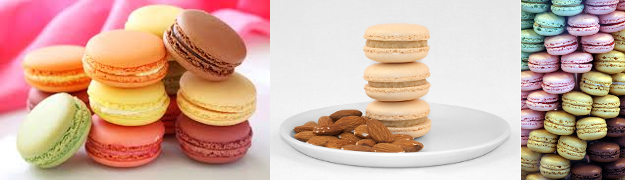
\includegraphics[scale=0.4]{macaron-stacks.png}~\footnote{
  \tiny Von links nach rechts: \\
By Mariajudit - Own work, CC BY-SA 4.0, https://commons.wikimedia.org/w/index.php?curid=48726001
  \\
By Michelle Naherny - Own work, CC BY-SA 4.0, https://commons.wikimedia.org/w/index.php?curid=44361114
  \\
By Keven Law - originally posted to Flickr as What's your Colour???, CC BY-SA 2.0, https://commons.wikimedia.org/w/index.php?curid=6851868
}
% Bunch - By Mariajudit - Own work, CC BY-SA 4.0, https://commons.wikimedia.org/w/index.php?curid=48726001
% Almond - By Michelle Naherny - Own work, CC BY-SA 4.0, https://commons.wikimedia.org/w/index.php?curid=44361114

\end{center}
Ein passendes Alphabet wäre $\Sigma = \{\mathtt{grün} , \mathtt{nicht-grün} \}$.
Wir definieren die folgenden Zustände.
(die Metapher hier ist: ,,wenn ich mehr als einen grünen Maccaron esse wird mir übel, und das wäre nicht akzeptabel'')
\begin{center}
\begin{tabular}{cl}
  Zustand & Bedeutung \\
  \hline
  $q_0$& ,,alles gut'' \\
  $q_1$& ,,mir wird schon flau'' \\
  $q_2$& ,,mir ist übel''
\end{tabular}
\end{center}
Der Startzustand ist $q_0$.
Akzeptierende Zustände sind $q_0$ und $q_1$.
Die Transistionsfunktion $\delta$ ist
\begin{center}
\begin{tabular}{cccl}
  &\texttt{grün} & \texttt{nicht-grün} \\
  \hline
  $q_0$ & $q_1$ & $q_0$ & wechsle nach $q_1$ falls \texttt{grün}, ansonsten verweile \\
  $q_1$ & $q_2$ & $q_1$ & wechsle nach $q_2$ falls \texttt{grün}, ansonsten verweile \\
  $q_2$  & $q_2$ & $q_2$ & verweile, da es nichts mehr zu retten gibt
\end{tabular}
\end{center}
\end{Bsp}

% \begin{Bsp}
% 	$L=\{w\in\{0,1\}^* \mid w \text{ enthält gerade Anzahl von 0 und gerade Anzahl von 1}\}$

% 	\begin{minipage}[t]{.4\textwidth}\centering\vspace{0pt}
% 	    \captionsetup{type=figure}
% 		\begin{tikzpicture}[circle/.style={
% 			shape=circle,
% 			minimum size=0.5cm,
% 			text=black, draw,
% 			text width=0.5cm,
% 			align=center}]
% 			\node (v1) at (-3.5,3.5) {};
% 			\node [circle,double] (v2) at (-2.5,3) {$q_{00}$};
% 			\node [circle] (v3) at (0.5,3) {$q_{01}$};
% 			\node [circle] (v4) at (0.5,0.5) {$q_{10}$};
% 			\node [circle] (v5) at (-2.5,0.5) {$q_{11}$};
% 			\draw [->] (v1) edge (v2);
% 			\draw [->] (v2) edge [bend left=15] node[auto] {1} (v3);
% 			\draw [->] (v3) edge [bend left=15] node[auto] {1} (v2);
% 			\draw [->] (v3) edge [bend left=15] node[auto] {0} (v4);
% 			\draw [->] (v4) edge [bend left=15] node[auto] {0} (v3);
% 			\draw [->] (v2) edge [bend left=15] node[auto] {0} (v5);
% 			\draw [->] (v5) edge [bend left=15] node[auto] {0} (v2);
% 			\draw [->] (v5) edge [bend left=15] node[auto] {1} (v4);
% 			\draw [->] (v4) edge [bend left=15] node[auto] {1} (v5);
% 		\end{tikzpicture}
% 		\captionof{figure}{Automat zu $L$}
% 	\end{minipage}\begin{minipage}[t]{.55\textwidth}\vspace{0pt}
% 	Graphische Darstellung $\hat=$ gerichteter Graph mit Knoten $Q$ und markierten Kanten gemäß $\delta$.\\
% 	$Q=\{q_{00},q_{01},q_{10},q_{11}\}$\\
% 	$q_{00}$ einziger akzeptierender Zustand ($F=\{q_{00}\}$)
% 	\end{minipage}
	
% 	\begin{tabular}{M{l}|M{l}|M{l}l @{\quad}l}
% 		& 0 & 1 &\\ \cline{1-3}
% 		q_{00} & q_{10} & q_{01} && gerade Anzahl von 0 und 1 gesehen\\
% 		q_{01} & q_{11} & q_{00} && gerade \ruleplaceholder{\widthof{Anzahl von 0}}, ungerade Anzahl von 1 gesehen\\
% 		q_{10} & q_{00} & q_{11} && ungerade \ruleplaceholder{\widthof{Anzahl von 0}}, gerade \ruleplaceholder{\widthof{Anzahl von 1 gesehen}} \\
% 		q_{11} & q_{01} & q_{10} && ungerade \ruleplaceholder{\widthof{Anzahl von 0}}, ungerade \ruleplaceholder{\widthof{Anzahl von 1 gesehen}}
% 	\end{tabular}
% \end{Bsp}
\begin{Def}[\acs*{DEA}]
	Ein \emph{\acf{DEA}}, (\acsu{DFA} $\hat=$ \acl{DFA}) ist ein 5-Tupel
	\[ M= (Q,\Sigma,\delta,q_0,F) \]
	\begin{itemize}
		\item $Q$ \emph{endliche} Zustandsmenge
		\item $\Sigma$ \emph{endl.} Alphabet
		\item $\delta:Q\x\Sigma\->Q$ Transitionsfunktion
		\item $q_0\in Q$ Startzustand
		\item $F\subseteq Q$ akzeptierende Zustande
	\end{itemize}
\end{Def}

DEAs lassen sich auch graphisch darstellen.
Dabei gibt man für den Automaten einen gerichteten Graphen an.
Die Knoten Graphen sind die Zustände und mit Zeichen gelabelte Kanten zeigen welchen Zustandsübergang die Transitionsfunktion für das nächste Zeichen erlaubt.
Der Startzustand ist mit einem ungelabelten Pfeil markiert und finale Zustände sind doppelt eingekreist.
Hier ist die graphische Darstellung von $A_{\mathtt{Maccaron}}$ aus Beispiel \ref{Bsp:3.1}

\begin{center}
\begin{tikzpicture}[node distance = 3cm]
  \node[state, accepting] (0) {$q_0$};
  \node[state, accepting, right of = 0] (1) {$q_1$};
  \node[state, right of = 1] (2) {$q_2$};

  \node[left of = 0, node distance = 1cm] (start){}; 
  \draw[->] (start) to (0);

  \draw[->] (0) to node[above] {\texttt{grün}} (1);
  \draw[->, loop above] (0) to node[above] {\texttt{nicht-grün}} (0);

  \draw[->] (1) to node[above] {\texttt{grün}} (2);
  \draw[->, loop above] (1) to node[above] {\texttt{nicht-grün}} (1);

  \draw[->, loop right] (2) to node[right]{\texttt{grün}, \texttt{nicht-grün}} (2);
\end{tikzpicture}
\end{center}

DEAs charakterisieren die Sprachen durch die Menge an Wörtern, die sie akzeptieren.
\begin{Bsp}
    Sei $M=(Q,\Sigma,\delta,q_0,F)$ ein DEA.
    \begin{itemize}
    \item Wenn $F=Q$, dann ist $L(M)=\Sigma^*$.
    \item Wenn $F=\emptyset$, dann ist $L(M)=\emptyset$.
    \end{itemize}
\end{Bsp}
\begin{Def}[name={[Erweiterung von $\delta$ auf Worte]}]
	Die Erweiterung von $\delta:Q\x\Sigma\->Q$ auf Worte $\hat{\delta}: Q\x\Sigma^*\->Q$ ist induktiv definiert durch
  \begin{enumerate}
  \item $\hat\delta(q,\Eps) =q$ (Wortende erreicht)
  \item $\hat\delta(q,aw)=\hat\delta(\delta(q,a),w)$ (Rest im Folgezustand verarbeiten)
  \end{enumerate}
\end{Def}
\begin{Def}[name={[Die durch einen \acs*{DEA} erkannte Sprache]}]
	Sei $M=(Q,\Sigma,\delta,q_0,F)$\\
	Die \emph{von $M$ erkannte Sprache} ist
	\[ L(M) = \{ w\in\Sigma^* \mid \hat\delta(q_0,w)\in F \} \]
	Eine durch einen \ac{DEA} erkannte Sprache heißt \emph{regulär}.
\end{Def}
Es folgen zwei Beispiele für reguläre Sprachen:
\begin{Bsp} 
\label{bsp:3.1}
	$L=\{w\in\{0,1\}^* \mid w \text{ enthält gerade Anzahl von 0 und gerade Anzahl von 1}\}$
  \begin{center}
		\begin{tikzpicture}[circle/.style={
			shape=circle,
			minimum size=0.5cm,
			text=black, draw,
			text width=0.5cm,
			align=center}]
			\node (v1) at (-3.5,3.5) {};
			\node [circle,double] (v2) at (-2.5,3) {$q_{00}$};
			\node [circle] (v3) at (0.5,3) {$q_{01}$};
			\node [circle] (v4) at (0.5,0.5) {$q_{10}$};
			\node [circle] (v5) at (-2.5,0.5) {$q_{11}$};
			\draw [->] (v1) edge (v2);
			\draw [->] (v2) edge [bend left=15] node[auto] {1} (v3);
			\draw [->] (v3) edge [bend left=15] node[auto] {1} (v2);
			\draw [->] (v3) edge [bend left=15] node[auto] {0} (v4);
			\draw [->] (v4) edge [bend left=15] node[auto] {0} (v3);
			\draw [->] (v2) edge [bend left=15] node[auto] {0} (v5);
			\draw [->] (v5) edge [bend left=15] node[auto] {0} (v2);
			\draw [->] (v5) edge [bend left=15] node[auto] {1} (v4);
			\draw [->] (v4) edge [bend left=15] node[auto] {1} (v5);
		\end{tikzpicture}
  \end{center}
\end{Bsp}
\begin{Bsp}\label{bsp:3.2}
	
	Sei $A\ge 0$ nat. Zahl, $\Sigma=\{0,1,\dots,A\}$
	\begin{equation*}
		L = \{ a_1\dots a_n \mid \exists J\subseteq \{1,\dots,n \},\ \sum_{i\in J} a_i = A \} \subseteq \Sigma^* 
	\end{equation*}
	D.h. gegeben eine Liste von Zahlen $\in\Sigma$.
	Akzeptiere diejenigen Listen, für die eine Teilliste existiert, deren Summe genau $A$ ist.
	\begin{align*}
		Q &=\Powerset\{0,1,\dots,A\} \\
		\delta(q,a) &= q \cup \{ x\in \{0,\dots,A\} \mid x-a \in q \} \\
		q_0 &=\{0\} \\
		F &= \{ q\in Q \mid A \in q \}
	\end{align*}
  $q \in Q$ bezeichnet die Menge an möglichen Summen $\le A$, die mit den bisher gelesenen Zeichen gebildet werden kann.
  Die Transitionsfunktion $\delta$ fügt die Summen zum aktuellen Zustand hinzu, die sich durch addieren der aktuell gelesenen Ziffer zu den alten Möglichkeiten ergeben.
\end{Bsp}
\begin{Bsp}\label{bsp:3.3}
	Beispiel f"ur eine nicht-regul"are Sprache.
	\begin{equation*}
		L = \{ 0^n1^n \mid n\in\N \} 
	\end{equation*}
	erkennbar durch \ac{TM} die immer anhält, \emph{aber nicht} von einem \ac{DEA} [\emph{nicht} regulär] akzeptiert werden kann.
	\begin{proof}
		Angenommen $L=L(M)$ für \ac{DEA} $M=(Q,\Sigma,q_0,\delta,F)$
		
		Beobachtung: $\exists m\neq n$, so dass $\hat\delta(q_0,0^m)=\hat\delta(q_0,0^n)=q'$ weil $Q$ endlich.
		\begin{itemize}
			\item Falls nun $\hat\delta(q',1^m)\in F$, dann ist auch $\hat\delta(q_0,0^n1^m)\in F$ und somit $0^n1^m\in L(M)$ mit $n\neq m\ \lightning$
			\item Falls $\hat\delta(q',1^m)\notin F$, dann gilt auch $\hat\delta(q_0,0^m1^m)\notin F$ und somit $0^m1^m \notin L$ $\lightning$
		\end{itemize}
		Also kann $M$ nicht existieren!
	\end{proof}
\end{Bsp}

\subsection{Minimierung endlicher Automaten}
 \datenote{26.10.16}

Betrachte den Automaten aus Beispiel \ref{bsp:3.2}.
Sei $A =4$, $\Sigma = \{0, 1, 2, 3, 4\}$ mit Zustandsmenge $Q = \Powerset(\Sigma)$.
D.h.\ unter anderem: $\{0, 1, 3\} \in Q$.
Hier ist ein Ausschnitt aus dem Zustandsdiagramm:

\begin{center}
\begin{tikzpicture}[node distance = 2cm]
  \node (0) at (0, 0) {$\{0\}$};
  \node[below of = 0] (03) {$\{0,3\}$};
  \node[right of = 03] (02) {$\{0,2\}$};
  \node[below of = 02] (0134) {$\{0,1,3,4\}$};
  \node[right of = 0] (01) {$\{0,1\}$};
  \node[right of = 01] (012) {$\{0,1,2\}$};
  \node[below of = 012] (0123) {$\{0,1,2, 3\}$};

   \draw[->] (- 0.8, 0) to (0);
  \draw[->] (0) to node[left] {$3$} (03);
  \draw[->] (0) to node[above] {$2$} (02);
  \draw[->] (0) to node[above] {$1$} (01);
  \draw[->] (03) to node[left] {$1$} (0134);
  \draw[->] (01) to node[above] {$1$} (012);
  \draw[->] (02) to node[above] {$1$} (0123);
\end{tikzpicture}
\end{center}
Es ist zu bemerken, dass manche Zustände von $Q$ nie erreicht werden können, z.B.\ $\emptyset$.
Sei für die folgenden Überlegungen $M = (Q, \Sigma, \delta, q_0, F)$ ein DEA.

\begin{Def}
  Ein Zustand $q \in Q$ ist \emph{erreichbar}, falls ein $w \in \Sigma^*$ existiert, so dass $\hat \delta(q_0, w) = q$.
  $M$ heißt \emph{reduziert}, falls alle Zustände erreichbar sind.
\end{Def}
\begin{Satz}
  Die Menge der erreichbaren Zustände kann in $O(|Q|*|\Sigma|)$ berechnet werden.
\end{Satz}
\begin{proof}~\\
  \vspace{-\baselineskip}
  \begin{itemize}
  \item Fasse $A$ als Graphen auf.
  \item Wende Tiefensuche an, markiere dabei alle besuchten Zustände.
  \item Die markierten Zustände ist die Menge der erreichbaren Zustände.
  \end{itemize}
\end{proof}

\ldots 



\draftnote{28.10.16}

\emph{Beobachtung:} Auch ein Automat mit lauter erreichbaren Zuständen muss nicht minimal sein

\begin{Bsp}\label{Bsp:3.4}\
	\begin{figure}[H]\centering
		\begin{tikzpicture}
			\node (start) at (-4,1.5) {};
			\node (q0) [circle,double] at (-3,1) {$q_0$};
			\node (q1) [circle,double] at (-0.5,1) {$q_1$};
			\node (q2) [circle] at (2,1) {$q_2$};
			\node (q3) [circle] at (3.5,1) {$q_3$};
			\draw [->] (start) edge (q0);
			\draw [->] (q0) edge[loop above] node {0} (q0);
			\draw [->] (q0) edge node [auto] {1} (q1);
			\draw [->] (q1) edge[loop above] node {0} (q1);
			\draw [->] (q1) edge node [auto] {1} (q2);
			\draw [->] (q2) edge[loop above] node {1} (q2);
			\draw [->] (q2) edge[bend left] node [auto] {0} (q3);
			\draw [->] (q3) edge[bend left] node [auto] {1,0} (q2);
		\end{tikzpicture}\\
		höchstens eine "`1"'
		\caption{Automat zu Bsp. \ref{Bsp:3.4}}
	\end{figure}
	Erkennt die gleiche Sprache wie in \eqref{bsp:3.1}, hat nur erreichbare Zustände, aber mehr Zustände als in \eqref{bsp:3.1}.
	
	\emph{Beobachtung:} $q_2$ und $q_3$ verhalten sich gleich in dem Sinn, dass
	\[ \forall w: \hat\delta(q_2,w) \notin F\text{ und }\hat\delta(q_3,w)\notin F \]
\end{Bsp}
%
%\stepcounter{Def}
%
\begin{Def}[name={[Äquivalenz von \acs*{DFA}-Zuständen]}] %\rlnote{Def.-Num. überprüfen}
	Zwei Zustände $q,p\in Q$ eines \ac{DFA} sind \emph{äquivalent}, geschrieben $p\equiv q$, falls $\forall w\in\Sigma^*$, $\hat\delta(p,w)\in F \<=> \hat\delta(q,w)\in F$
\end{Def}
%\stepcounter{lemma}

\begin{lemma}[name={[$\equiv$ ist Äquivalenzrelation]}] %\rlnote{Satz = Lemma-Nummer: 3.2 statt 3.1?}
	$\equiv$ ist Äquivalenzrelation\\
	\framebox{\parbox{.96\linewidth}{Eine Relation ist genau dann eine Äquivalenzrelation, wenn sie reflexiv, transitiv und symmetrisch
	ist.}}
\end{lemma}
\begin{proof} $\equiv$ ist offensichtlich reflexiv.
	
	$\begin{rcases}
	\text{transitiv}\\
	\text{symmetrisch}
	\end{rcases}$ wegen \<=>
	
	Also $q_2,q_3$ aus \autoref{Bsp:3.4} sind äquivalent.
\end{proof}
\begin{Erinnerung}
Hauptlemma "uber "Aquivalenzrelationen
\begin{align*}
	[q] &= \{p\in Q \mid p \equiv q\} &&[q] \text{ ist Äquivalenzklasse von }q
\end{align*}
"Aquivalenzklassen sind paarweise disjunkt:

F"ur alle $ p,q\in Q$ gilt entweder $[p]=[q]$ oder $[p]\cap[q] = \emptyset$ (folgt aus Transitivität).

D.h. $Q$ wird in disjunkte Äquivalenzklassen aufgeteilt. Anzahl der Äquivalenzklassen ist der \textbf{Index}.
\end{Erinnerung}

\eqref{bsp:3.1}:
\begin{minipage}{.5\textwidth}
    \captionsetup{type=figure}
	\begin{tikzpicture}
		\node (start) at (-4,1.5) {};
		\node (q0) [circle,double] at (-3,1) {$q_0$};
		\node (q1) [circle,double] at (-0.5,1) {$q_1$};
		\node (q2) [circle] at (2,1) {$q_2$};
		\draw [->] (start) edge (q0);
		\draw [->] (q0) edge[loop above] node {0} (q0);
		\draw [->] (q1) edge[loop above] node {0} (q1);
		\draw [->] (q2) edge[loop above] node {0,1} (q2);
		\draw [->] (q0) edge node [auto] {1} (q1);
		\draw [->] (q1) edge node [auto] {1} (q2);
	\end{tikzpicture}
	\captionof{figure}{Automat zu \eqref{bsp:3.1}}
\end{minipage}

Allgemein gilt f"ur alle $p,q\in Q$:
\begin{align}
\label{eqn:delta-wohldefiniert}
	p &\equiv q \=> \forall a\in\Sigma:\ \delta(p,a)\equiv\delta(q,a)
\end{align}
Denn
\begin{align*}
	p \equiv q  
	& \<=> \forall w\in\Sigma^*: \hat\delta(p,w)\in F \<=> \hat\delta(q,w) \in F\\
	& \<=> (p\in F \<=> q \in F) \land \forall a\in \Sigma: \forall w\in\Sigma^*:
	\hat\delta(p,aw)\in F \<=> \hat\delta(q,aw)\in F\\
	&\=>  \forall a\in\Sigma: \forall w\in\Sigma^*: \hat\delta(\delta(p,a),w)\in F \<=> \hat\delta(\delta(q,a),w)\in F\\
	& \<=>\forall a\in\Sigma: \delta(p,a)\equiv\delta(q,a)
\end{align*}
Also können wir äquivalente Zustände zusammenfassen und Transitionen verschmelzen, wie in der folgenden Definition formalisiert.
\begin{Def}[name={[Äquivalenzklassenautomat]}]
	Der Äquivalenzklassenautomat $M'=(Q',\Sigma,\delta',q_0',F')$ zu $M$ ist bestimmt durch:
	\begin{align*}
		Q' &= \{[q]\mid q\in Q\} & \delta'([q],a) &= [\delta(q,a)]\\
		q_0' &= [q_0] & F'&=\{[q]\mid q\in F \}
	\end{align*}
\end{Def}
Dabei ist $[q]=\{p\in Q \mid p\equiv q\}$
\begin{Satz}[name={[Äquivalenzklassenautomat ist wohldefiniert]}]
	Der Äquivalenzklassenautomat ist wohldefiniert und $L(M)=L(M')$.
\end{Satz}
\begin{proof}\ 
	\begin{enumerate}
		\item Wohldefiniert: zu zeigen $\delta'([q],a) =[\delta(q,a)]$ ist nicht abhängig von der Wahl des Repräsentanten $q\in [q]$. Das folgt direkt aus \eqref{eqn:delta-wohldefiniert} gezeigt.
		\item $L(M)=L(M')$ zeige für alle $w\in\Sigma^*$ und alle $q$: $\hat\delta(q,w)\in F \<=> \hat\delta'([q],w)\in F'$\\
		Induktion über $w$:\\
		I.A. $w=\Eps$: $\hat\delta(q,\Eps)=q\in F \<=> \hat\delta'([q],\Eps)=[q]\in F'$ nach Definition.\\
		I.V.: $\forall w'\in\Sigma$, $\forall q\in Q$, $\hat\delta(q,w')\in F \<=> \hat\delta'([q],w')\in F'$\\
		I.S.: \begin{align*}
		\hat\delta(q,aw')\in F &\<==> \hat\delta(\delta(q,a),w')\in F\\ &\xLeftrightarrow{I.V.} \hat\delta'([\delta(q,a)],w')\in F'\\
		&\<==> \hat\delta'(\delta'([q],a),w')\in F'\\
		&\<==> \hat\delta'([q],a w')\in F'
		\end{align*}
		Also f"ur $q=q_0$: $\forall w\in\Sigma^*$, $w\in L(M)\<==> \hat\delta(q_0,w) \in F \<=> \hat\delta'([q_0],w) \in F' \<==> w\in L(M')$
	\end{enumerate}
\end{proof}
\emph{Bem:} Die Konstruktion von $M'$ kann in $O(|Q||\Sigma|\log|Q|)$ passieren.

Warum ist nun der Äquivalenzklassenautomat minimal?\\
\-> Satz von Myhill-Nerode
\begin{Def}[name={[Rechtsinvariante Äquivalenzrelation]}]
	Eine Äquivalenzrelation $R\subseteq\Sigma^*\x\Sigma^*$ heißt rechtsinvariant, falls
	\[ (u,v)\in R \=> \forall w\in\Sigma^*,(u\cdot w,v\cdot w) \in R \]
\end{Def}
%\setcounter{Bsp}{5}
\begin{Bsp} %\rlnote{Bsp.-Num. überprüfen (3.6)}
  \label{Bsp:R_m}
	Für einen \ac{DEA} $M$ definiere
	\[ R_M = \{(u,v) \mid \hat\delta(q_0,u)=\hat\delta(q_0,v)\} \]
	\begin{itemize}
		\item ist Äquivalenzrelation
		\item ist rechtsinvariant
		\item Anzahl der Äquivalenzklassen(Index von $R_M$)\\
		= Anzahl der "`nützlichen"' Zustände, die von $q_0$ erreichbar sind.
	\end{itemize}
\end{Bsp}
\begin{Bsp}
	Für eine Sprache $L\subseteq \Sigma^*$ definiere die Nerode Relation
	\[ R_L = \{(u,v) \mid \forall w\in\Sigma^*: uw\in L \<=> vw\in L \} \]
	\begin{itemize}
		\item ist Äquivalenzrel.
		\item ist rechtsinvariant. Sei $(u,v)\in R_L$\\
		Zeige $\forall w\in\Sigma^*\ (uw,vw)\in R_L$\\
		Induktion:\\
		I.A. $w=\Eps$: $ (u\Eps,v\Eps)=(u,v)\in R_L$\\
		I.S. $w=w'a$:\\
		I.V.: $(uw', vw') \in R_L $
		\begin{align*}
			(uw',vw')\in R_L 
			&\<=> \forall z\in\Sigma^*, \quad uw'z\in L \<=> vw'z\in L\\
			&\=> \forall a\in \Sigma, z'\in\Sigma^*: uw'az'\in L \<=> vw'az'\in L\\
			& \<=>\ (uw'a,vw'a)\in R_L
		\end{align*}
	\end{itemize}
\end{Bsp}

\begin{alignat*}{2}
	&\begin{rcases}
	L=\{\Eps\} & [\Eps]\equiv[\Eps]\\
	w,v\in\Sigma^*,\ w,v\ne\Eps & [w]=[v]
	\end{rcases} &\ &\text{Index}= 2\\
	&L = \varnothing, L= \Sigma^* &&\text{Index}= 1
\end{alignat*}

\begin{Satz}[Nerode] % 3.4
	Die folgende Aussagen sind äquivalent:
	\begin{enumerate}
		\item\label{itm:Nerode1} $L\subseteq \Sigma^*$ wird von \ac{DEA} akzeptiert.
		\item\label{itm:Nerode2} $L$ ist Vereinigung von Äquivalenzklassen einer rechtsinvarianten Äquivalenzrelation mit \emph{endlichem} Index.
		\item\label{itm:Nerode3} Die Nerode Relation $R_L$ hat \emph{endlichen} Index
	\end{enumerate}
\end{Satz}

\draftnote{2.11.16}
\begin{proof}
  Wir beweisen die gegenseitige Äquivalenz in drei Schritten:

  \begin{center}
    (1) \=> (2) \quad \mbox{(2) \=> (3)} \quad (3) \=> (1)
  \end{center}

	\paragraph{(1) \=> (2)}: Sei $M$ ein \ac{DEA} mit
  \begin{displaymath}
    L(M)=\{w \mid \hat\delta(q_0,w)\in F \} = \bigcup_{q \in F} \{ w \mid \hat\delta(q_0,w) = q\}
\end{displaymath}

Nun sind $\{ w \mid \hat\delta(q_0,w)=q \} = [q]_M$ genau die Äquivalenzklassen von $R_M$ aus Bsp \ref{Bsp:R_m}, einer rechtsinvarianten Äquivalenzrelation.
Der Index ist die Anzahl der erreichbaren Zustände.

Also: $\operatorname{Index}(R_M) \le |Q| < \infty$.
	
\paragraph{(2) \=> (3)} Sei $R$ rechtsinvariante Äquivalenzrelation mit endlichem Index, so dass $L=\bigcup R$-Äquivalenzklassen
	
Es genügt zu zeigen, dass wenn $(u,v)\in R$ auch $(u,v)\in R_L $.\footnote{
Zur Erklärung: falls $R \subseteq R'$, dann $\operatorname{Index}(R) \ge \operatorname{Index}(R_L)$.
Intuitiv: $R$ unterscheidet mehr Elemente und hat demnach auch mehr unterschiedliche Klassen.}

\begin{itemize}
\item[] $R$ rechtsinvariant
\item[gdw] für alle  $w\in\Sigma^*$ : $(uw,vw)\in R$ 
\item[gdw] für alle $w\in\Sigma^*$: $uw\text{ und $vw$ in gleicher $R$-Klasse}$
\end{itemize}
Da $L$ aus der Vereinigung von $R$-Klassen besteht folgt daraus:
\begin{itemize}
  \item[] für alle $w\in\Sigma^*$: $uw\in L\<=>vw\in L$
  \item[gdw] $(u, v) \in R_L$ (per Definition von $R_L$)
\end{itemize}

Also gilt: $\text{\#Klassen($R_L$)$\leq$\#Klassen($R$)}<\infty$

\paragraph{(3) \=> (1)} Gegeben $R_L$\\
		Konstruiere $\A'=(Q,\Sigma,\delta',q_0',F')$
		\begin{alignat*}{3}
			&&Q' &= \{ [w]_{R_L} \mid w\in \Sigma^* \} &\quad& \text{endlich, weil index($R_L$) endl.}\\
			&&\delta'([w],a) &= [wa] && \text{wohldefiniert, da $R_L$ rechtsinvariant}\\
			&&q_0' &= [\Eps]\\
			&&F' &= \{ [w] \mid w\in L \}\\
			\shortintertext{Zeige $L(\A')=L$, d.h. }
			&\forall w\in \Sigma^* &: w\in L(\A') &\<=> \hat\delta([\Eps],w)\in F'\\
			&&&\overset{???}{\<=>} [w]\in F' \\
			&&&\<=> w\in L
		\end{alignat*}
		Zeige nun noch, dass $???$ gilt: $\hat\delta([\Eps], w) = [w]$. 
		Daf"ur m"ussen wir wie folgt verallgemeinern um eine funktionierende Induktionsvoraussetzung zu erhalten.
		\begin{alignat*}{3}
			&&\forall w\in\Sigma^* &:
			\forall v\in\Sigma^* : \hat\delta'([v],w) = [v\cdot w]\\
			\shortintertext{Induktion über $w$}
			&\text{I.A.: }& \Eps &: \hat\delta'([v],\Eps) = [v]=[v\cdot\Eps]\\
			&\text{I.S.: }& \hat\delta'([v],aw') &= \hat\delta'(\delta'([v],a),w')\\
			&&&= \hat\delta'([v\cdot a],w')\\
			&&&\overset{\mathrlap{\text{I.V.}}}{=} [va\cdot w']\\
			&&&= [v\cdot \underbrace{aw'}_{=w}]
		\end{alignat*}
		Das gewünschte Ergebnis \framebox{???} ergibt sich für $v=\Eps$. \qedhere
\end{proof}
%
\setcounter{Korollar}{4}
\begin{Korollar}
	Der im Beweisschritt (3) \=> (1) konstruierte Automat $\A'$ ist minimaler Automat für $L$.
\end{Korollar}
\begin{proof}
	$L$ regulär. Sei $\A$ \emph{beliebiger \ac{DFA} mit $L=L(\A)$}\\
	$\begin{rcases}
	\A\text{ induziert }R_\A\text{ mit}\\
	|Q|\geq\text{index}(R_\A)
	\end{rcases}$ $\ref{itm:Nerode1} \overset{vgl.}{\<=>} \ref{itm:Nerode2}$
	
	In \ref{itm:Nerode2} \=> \ref{itm:Nerode3}: $R_\A\subseteq R_L$,\ index($R_\A$) $\geq$ index($R_L$)\\
	In \ref{itm:Nerode3} \=> \ref{itm:Nerode1} $A'$ mit $|Q'|=\text{index}(R_L) \leq \text{index}(R_\A)\leq |Q|$
	
	Minimalität von $A'$ folgt aus freier Wahl von $\A$
\end{proof}

Angenommen $\exists\,\A$ mit $L=L(\A)$ und $|\A|<|\A'|$\\
Nach Folgerung gilt aber
\[ |\A'| \leq |\A|\ \lightning \]

\subsection{\acf{PL} für reguläre Sprachen} %\rlnote{subsection \# (3.3)?}
\datenote{26.10.16 (Eingeschoben)}
Suche: Notwendiges Kriterium für Regularität
\begin{Bsp*}
		$L = \{ w\in \{0,1\}^* \mid \operatorname{bin}(w)\equiv_3 0\}$ ist regulär, dabei ist "`bin"' die Dekodierung von einem Bitstring in eine nat"urliche Zahl.
    \begin{center}
		\begin{tikzpicture}
			\node (start) at (-4,1.5) {};
			\node (q0) [circle, double] at (-3,1) {$q_0$};
			\node (q1) [circle] at (-0.5,1) {$q_1$};
			\node (q2) [circle] at (2,1) {$q_2$};
			\draw [->] (start) edge (q0);
			\draw [->] (q0) edge [loop above] node {0} (q0);
			\draw [->] (q0) edge node [auto] {1} (q1);
			\draw [->] (q1) edge [bend left] node [auto] {1} (q0);
			\draw [->] (q1) edge node [auto] {0} (q2);
			\draw [->] (q2) edge [bend left] node [auto] {0} (q1);
			\draw [->] (q2) edge [loop above] node {1} (q2);
		\end{tikzpicture}
  \end{center}
  \begin{itemize}
  \item Es gilt offensichtlich, dass $11 \in L$
  \item Es auch, dass $1 \underline{0 0} 1 \in L$.
  \item Der Automat hat eine Schleife bei $\hat\delta({q_1,00}) = q_1$, die mehrfach ,,abgelaufen'' werden kann ohne die Akzeptanz zu beinflussen.
  \item Also gilt auch $100001 \in L$,
  \item und im Allgemeinen $\forall i\in\N: 1(00)^i1 \in L$
  \end{itemize}
\end{Bsp*}

\begin{lemma}[Pumping Lemma]\label{lem:pumping}
	Sei $L$ regulär:
	\begin{alignat*}{2}
		&\exists n\in\N,\ n>0\quad \forall z\in L,\ |z|\geq n:\\
		&\exists u,v,w\in\Sigma^* :\\
		&z = uvw,\ |uv| \leq n,\ |v| \geq 1\\
		\text{sodass }& \forall i\in\N:\ uv^iw\in L
	\end{alignat*}
\end{lemma}
\vspace{-1em}
\begin{proof}
	Sei $\A=(Q,\Sigma,\delta,q_0,F)$ ein \ac{DFA} für $L$.\\
	Wähle $n=|Q|$ und $z\in L$ mit $|z|\geq n$.
	
	Beim Erkunden von $z$ durchläuft $\A\ \underbrace{|z|+1}_{\geq n+1}$ Zustände.\\
	\-> $\exists\, q$, das mehrmals besucht wird.
	
	Wähle das $q$, dessen zweiter Besuch zuerst passiert.
	\begin{alignat*}{3}
		\text{D.h.}:&\quad& \hat\delta(q_0,u)&=q &\qquad& u\text{ Präfix von }z\\
		\exists v:&& \hat\delta(q,v)&=q && uv\text{ Präfix von }z\\
		\exists w:&& \hat\delta(q,w)&\in F && uvw=z\\
		&& |v| &\geq 1\\
		&& |uv| &\leq n && \text{ergibt sich aus Wahl von }q
	\end{alignat*}
	\begin{alignat*}{2}
		\text{jetzt:}\quad &\hat\delta(q_0,uv^iw) &\quad& i\in\N\\
		&= \hat\delta(q,v^iw)\\
		&= \hat\delta(q,w) && \text{denn }\forall i: \hat\delta(q,v^i)=q\\
		&\in F \tag*{\qedhere}
	\end{alignat*}
\end{proof}
%
\begin{Bsp*}
	$L=\{0^n10^n \mid n\in\N\}$ ist nicht regulär.\\
	Sei $n$ die Konstante aus dem \ac{PL}.
	
	Wähle $z=0^n10^n$. Also $|z|=2n+1\geq n$\\
	Laut PL existieren $u$, $v$, $w$, sodass $z=uvw$ mit $|v|\geq 1, |uv|\leq n$ und $\forall i \in \N$ $uv^iw \in L$. Nach Wahl von $z$ gilt nun
  \begin{itemize}
  \item $uv = 0^m$ mit $m\leq n$
  \item $v = 0^k$ mit $k\geq 1$
  \item $w = 0^{n-m}10^n$ 
  \end{itemize}
  Betrachte $uv^2w = 0^{m+k}0^k0^{n-m}10^n = 0^{n+k}10^n \notin L$.
  Also ist $L$ nicht regulär.
  Zur Illustration:
	\begin{gather*}
		\underbrace{0\ \dots\dots\ 0}_{n} \ \underbrace{1\ \dots\dots\ 1}_{n}\\
		|\!\ruleplaceholder[u]{\widthof{0\ \dots }} \!|\! \ruleplaceholder[v]{\widthof{\dots 0}}\!|% 
		\ruleplaceholder[w]{\widthof{\ \ \ $1\ \dots\dots\ 1$}}\!|
	\end{gather*}
  
\end{Bsp*}
\begin{Bsp*}
	$L=\{0^{x^2} \mid x\in\N\}$ ist nicht regulär.\\
	Sei $n$ die Konstante aus dem \ac{PL}.
	
	Wähle $z=0^{n^2}$. Also $|z|=n^2\geq n$\\
	Laut PL existieren $u$, $v$, $w$, sodass $z=uvw$ mit $|v|\geq 1, |uv|\leq n$ und $\forall i \in \N$ $uv^iw \in L$. Nach Wahl von $z$ gilt nun
  \begin{itemize}
  \item $uv = 0^m$ mit $m\leq n$
  \item $v = 0^k$ mit $k\geq 1$
  \item $w = 0^{n^2 - m}$ mit $k\geq 1$
  \end{itemize}
  Betrachte $uv^2w = uvvw = 0^{m}0^k0^{n^2-m} = 0^{n^2+k}$.
  Da $n^2+k$ keine Quadratzahl sein kann ist $uv^2w \not \in L$, und somit ist $L$ nicht regulär.
  Begründung: betrachte $(n+1)^2 - n^2 = n^2 + 2n + 1 - n^2 = 2n + 1$.
  Aber $k \le m \le n \le 2n + 1$.
\end{Bsp*}

\begin{Bsp*}
$L_2 = \{0^p \mid p\text{ ist Primzahl}\}$ ist nicht regulär.

Sei $n$ Konst. aus dem \ac{PL}, $p$ Primzahl mit $p \geq n$.\\
Wähle $z=0^p \in L_2$
\begin{align*}
	\ac{PL}:\ &z=uvw \text{ mit } |uv|\leq n &&,|v| \geq 1\\
	&\curvearrowright |z|= p=a+b &&, a = |uw| \quad, b= |v|\\
	&\curvearrowright |uv^iw| = a + ib &&, \text{w"ahle }i=p+1\\
	&\curvearrowright |uv^{p+1}w| = a + (p+1)b & =& a + pb + b = p+pb \text{ keine Primzahl} \\
	\text{Also } &uv^{p+1}w \notin L_2\\
	&\curvearrowright L_2\text{ nicht regulär.}
\end{align*}
\end{Bsp*}

\subsection[\acf{NEA}]{\acf{NEA}\draftnote{2.11.16} (Vortsetzung)}
\begin{Bsp*} Mustererkennung\\
	kommt ein String (konsistent) in einem anderen vor?
	
	Gegeben: festes Wort $w$.\\
	Gesucht: Sprache aller Worte, in denen $w$ als Teilwort vorkommt.
	\begin{align*}
		L &= \{ v\in\Sigma^* \mid \exists u,x\in\Sigma^*, v=uwx \}\\
		\Sigma &= \{a,b,c\}\\
		& \text{konkretes Beispiel:}\\
		w &= abac
	\end{align*}
	\begin{figure}[tp]
	\centering
		\begin{tikzpicture}[>=stealth, shorten >=1pt,
				node distance=2cm, on grid, initial text=,
				every state/.style={minimum size=0pt,inner sep=0pt}
			]
			\node[state,initial] (q0) {};
			\node[state] (q1) [right of=q0] {};
			\node[state] (q2) [right of=q1] {};
			\node[state] (q3) [right of=q2] {};
			\node[state,accepting] (q4) [right of=q3] {};
			\path[->]
				(q0) edge [loop above]    node [auto]  {$b,c$}    ()
				     edge                 node [auto]  {$a$}      (q1)
				(q1) edge [loop above]    node [auto]  {$a$}      ()
				     edge [bend left]     node [auto]  {$c$}      (q0)
				     edge                 node [auto]  {$b$}      (q2)
				(q2) edge [bend left=50]  node [auto]  {$b,c$}    (q0)
				     edge                 node [auto]  {$a$}      (q3)
				(q3) edge                 node [auto]  {$c$}      (q4)
				     edge [bend right=70] node [above] {$a$}      (q1)
				     edge [bend right=40] node [above] {$b$}      (q2)
				(q4) edge [loop right]    node [auto]  {$\Sigma$} ()
			;
		\end{tikzpicture}
	\caption{DFA für $L$}
	\label{fig:dfa-teilwort}
	\end{figure}
	\hyperref[fig:dfa-teilwort]{Abbildung~\ref*{fig:dfa-teilwort}} enthält einen \ac{DFA} für die Sprache $L$. Beobachtung: nicht-trivial zu konstruieren.
	\begin{figure}[tp]\centering
		\begin{tikzpicture}[>=stealth,shorten >=1pt,
				node distance=2cm,on grid,
				initial text=
			]
			\node[state,initial] (q0) {$q_0$};
			\node[state] (q1) [right of=q0] {$q_1$};
			\node[state] (q2) [right of=q1] {$q_2$};
			\node[state] (q3) [right of=q2] {$q_3$};
			\node[state,accepting] (q4) [right of=q3] {$q_4$};
			\path[->]
				(q0) edge [loop above] node [auto] {$\Sigma$} ()
				     edge              node [auto] {$a$} (q1)
				(q1) edge              node [auto] {$b$} (q2)
				(q2) edge              node [auto] {$a$} (q3)
				(q3) edge              node [auto] {$c$} (q4)
				(q4) edge [loop above] node [auto] {$\Sigma$} ()
			;
		\end{tikzpicture}
		\caption{Bsp.: Mustererkennung}
		\label{fig:nfa-teilwort}
	\end{figure}
	
	\hyperref[fig:nfa-teilwort]{Abbildung~\ref*{fig:nfa-teilwort}} enthält einen nicht-deterministischen endlichen Automat für die Sprache $L$. Idee: Ein Wort $w$ wird akzeptiert, falls es einen mit $w$ markierten Pfad von $q_0$ zu einen akzeptierenden Zustand gibt.
	\begin{figure}[tp]
	\centering
		\begin{tikzpicture}[>=stealth,shorten >=1pt,
				node distance=2cm,on grid
			]
			\node (q0) {$\{0\}$};
			\node (q1) [right of=q0] {$\{0,1\}$};
			\node (q2) [right of=q1] {$\{0,2\}$};
			\node (q3) [right of=q2] {$\{0,1,3\}$};
			\path[->]
				(q0) edge [loop below] node [auto] {$b,c$} ()
				     edge              node [auto] {$a$} (q1)
				(q1) edge [loop below] node [auto] {$a$} ()
				(q1) edge              node [auto] {$b$} (q2)
				(q2) edge              node [auto] {$a$} (q3)
			;
		\end{tikzpicture}
	\caption{Potenzmengenkonstruktion auf dem NFA}
	\label{fig:nfa-teilwort-powerset}
	\end{figure}
	
	\hyperref[fig:nfa-teilwort-powerset]{Abbildung~\ref{fig:nfa-teilwort-powerset}} zeigt (einen Ausschnitt) aus dem deterministischen Automaten, der schematisch aus dem \acsu{NFA} in \autoref{fig:nfa-teilwort} konstruiert werden kann. Idee: bei Schritt mit Symbol $a$ ist der \ac{NFA} gleichzeitig in allen Zuständen, die durch $a$ von (der Menge der) aktuellen Zustände erreichbar sind.
	
	Variante: erkenne \textbf{Subwort} $w=a_1,\dots,a_n$
	\[ L' = \{ v\in\Sigma^* \mid \exists x_0,\dots,x_n\in\Sigma^*, v=x_0a_1x_1a_2\dots a_nx_n \} \]
	Nicht det. Automat für $L'$ mit $(w=abac)$ ist sehr einfach. Der entsprechende deterministische Automat ist deutlich komplizierter. (selbst)
	\begin{figure}[H]\centering
		\begin{tikzpicture}[>=stealth, shorten >=1pt,
				node distance=2cm, on grid, initial text=,
				every state/.style={minimum size=0pt,inner sep=0pt}
			]
			\node[state,initial] (q0) {};
			\node[state] (q1) [right of=q0] {};
			\node[state] (q2) [right of=q1] {};
			\node[state] (q3) [right of=q2] {};
			\node[state,accepting] (q4) [right of=q3] {};
			\path[->]
				(q0) edge [loop above] node [auto] {$\Sigma$} ()
				     edge              node [auto] {$a$}      (q1)
				(q1) edge [loop below] node [auto] {$\Sigma$} ()
				     edge              node [auto] {$b$}      (q2)
				(q2) edge [loop below] node [auto] {$\Sigma$} ()
				     edge              node [auto] {$a$}      (q3)
				(q3) edge [loop below] node [auto] {$\Sigma$} ()
				     edge              node [auto] {$c$}      (q4)
				(q4) edge [loop right] node [auto] {$\Sigma$} ()
			;
		\end{tikzpicture}
		\caption{Nichtdet. Automat für $L'$}
	\end{figure}
	
	Weiteres Beispiel, bei dem der deterministische Automat beweisbar exponentiell größer ist.
	\begin{align*}
		L_n &= \{ w\in\{0,1^* \mid \text{das $n$-letzte Symbol von $w$ ist 1} \}
	\end{align*}
	\begin{figure}[H]\centering
		\begin{tikzpicture}[>=stealth, shorten >=1pt,
				node distance=1.5cm, on grid, initial text=,
				every state/.style={minimum size=0pt,inner sep=0pt}
			]
			\node[state,initial] (q0) {};
			\node[state] (q1) [right of=q0] {};
			\node        (q2) [right of=q1] {\dots};
			\node[state,accepting] (q3) [right of=q2] {};
			\path[->]
				(q0) edge [loop above] node [auto] {$\Sigma$} ()
				     edge              node [auto] {1}        (q1)
				(q1) edge              node [auto] {$\Sigma$} (q2)
				(q2) edge              node [auto] {$\Sigma$} (q3)
			;
			\draw [thick, decoration={brace, mirror, raise=.3cm, amplitude=10pt}, decorate]
			    (q1.west) -- (q3.east)
			    node [pos=0.5,anchor=north,yshift=-0.65cm] {n};
		\end{tikzpicture}
		\caption{Nichtdet. Automat für $L_n$}
	\end{figure}
	
	deterministischer Automat für $L_n$ hat $\sim 2^n$ Zustände.
\end{Bsp*}

\begin{Def}[name={[NEA]}]
	Ein \ac{NEA} (\acsu{NFA} = \acl{NFA}) $\A = (Q,\Sigma,\delta,q_0,F)$ mit
	\begin{itemize}
		\item $Q$ endliche Zustandsmenge
		\item $\Sigma$ endl. Alphabet
		\item $\delta:Q\x\Sigma\->\mathcal{P}(Q)$ Transitionsfunktion
		\item $q_0\in Q$ Startzustand
		\item $F\subseteq Q$ akzeptierende Zust"ande
	\end{itemize}
\end{Def}
\begin{Def}[name={[Lauf eines Automaten]}]
	Ein \emph{Lauf des Automaten $\A$ auf $w=a_1\dots a_n$} ist eine Folge $q_0q_1\dots q_n$ mit $q_i\in Q$, $q_0$ Startzustand,\\
	$\forall 1\leq i\leq n,\ q_i\in\delta(q_{i-1},a_i)$\\
	Ein Lauf heißt \emph{akzeptierend}, falls $q_n\in F$.
\end{Def}
\begin{Def}[name={[NFA zu DFA]}]
	$L(\A)=\{ w\in\Sigma^* \mid \exists\text{ akzeptierender Lauf von $\A$ auf }w \}$
\end{Def}
\begin{Satz}[Rabin]
	Zu jedem \ac{NFA} $\A$ mit $n$ Zuständen gibt es einen \ac{DFA} $\A'$ mit $2^n$ Zuständen, so dass $L(\A)=L(\A')$.
\end{Satz}
\draftnote{4.11.16}
\begin{proof}[Potenzmengenkonstruktion]
	Definiere $\A'$ durch
	\begin{align*}
		Q' &= \mathcal{P}(Q)\\
		\delta'(q',a) &= \bigcup_{q\in q'} \delta(q,a)\\
		q_0' &= \{q_0\}\\
		F' &= \{ q'\in Q' \mid q'\cap F\neq \varnothing \}
	\end{align*}
	Zeige $L(\A)=L(\A')$
	\begin{align*}
		\text{Es gilt } w\in L(\A') &\<=> \hat\delta'(q_0',w)\in F'\\
		&\<=> \hat\delta'(q_0',w)\cap F\neq \varnothing\\
		w\in L(\A) &\<=> \exists \text{ akzeptierender Lauf von $\A$ auf $w$}.
		\intertext{Zeige $\forall w\in\Sigma^*$}
		\forall q'\in Q' &\phantom{\<=>} \hat\delta'(q',w)\cap F\neq \varnothing\\
		&\<=> \exists\text{ akzeptierender Lauf von $\A$ \underline{ab $q'$} auf }w\\
		&\<=> \exists \underbrace{p_0p_1\dots p_n}_{\text{Lauf}}\in Q \quad p_0=q',\ p_n\in F,\ n=|w|
	\end{align*}
	Induktion nach $w$
	\begin{description}
	\item[I.A.]
		\begin{alignat*}{2}
			\Eps:\\
			&&\forall q'\in Q'\ \hat\delta(&q',\Eps)\cap F\neq \varnothing\\
			\<=>&& &q'\cap F\neq \varnothing
		\end{alignat*}
		Wähle einen beliebigen Zustand $p_0=p_n\in q'\cap F$
	\item[I.S.]
	\begin{align*}
		aw'&\\
		&\hat\delta'(q',aw')\cap F\neq \varnothing\\
		\<=>\quad& \hat\delta'(\underbrace{\delta'(q',a)}_{\in Q'},w')\cap F\neq\varnothing\\
		\xLeftrightarrow{\text{I.V.}}\quad& \exists \text{Lauf\ } p_1\dots p_{n+1}\in Q : p_0\in\hat\delta'(q', a),\ p_{n+1}\in F
	\end{align*}
	Suche $p_0\in q'$ mit $p_1\in\delta(p_0,a)$\\
	existiert, denn
	\begin{align*}
		& p_1\in \delta'(q', a) =  \bigcup_{q\in q'} \delta(q,a)\\
		\<=>\quad & \exists p_0\in q' : \delta(p_0,a) \ni p_1\\
		\shortintertext{Gesuchter Lauf ist}
		p_0p_1\dots p_{n+1}
	\end{align*}
	\end{description}
\end{proof}
Also: Eine Sprache $L$ ist regulär, falls
\begin{itemize}
\item $L = L(\A)$ für einen \ac{DFA}\\
	oder
\item $L = L(\A)$ für \ac{NFA}
\end{itemize}

\subsection{Abschlusseigenschaften}
\begin{Def}[name={[Abgeschlossenheit von $\mathcal{L}$]}]
	Eine Menge $\mathcal{L}\subseteq \mathcal{P}(\Sigma^*)$ von Sprachen heißt \emph{abgeschlossen} unter Operation \\
	$f:\mathcal{P}(\Sigma^*)^n \-> \mathcal{P}(\Sigma^*)$ falls $\forall L_1,\dots, L_n\in \mathcal{L} : f(L_1,\dots, L_n)\in \mathcal{L}$.
\end{Def}
\begin{Satz}[name={[Abgeschlossenheit von $REG$]}]\label{satz:3.8}
	Die Menge $REG$ der regulären Sprachen ist abgeschlossen unter $\cup$ (Vereinigung), $\cap$ (Durchschnitt), $\overline{\phantom{X}}$ (Komplement), Produkt (Konkatenation), Stern.
\end{Satz}
\begin{proof}
	Sei $\A_i:=(Q_i,\Sigma,\delta_i,q_{0i},F_i)\quad i=1,2$ \acs{NFA}s
	\begin{itemize}
	\item $\cup:$ Def $\A$ durch (vgl.\ Abb.~\ref{fig:reg-closure-union})
		\begin{align*}
			Q &= Q_1\overset.\cup Q_2\overset.\cup\{q_0\}\\
			\delta(q,a) &=
                \begin{cases}
                    \delta_1(q,a) & q\in Q_1\\
                    \delta_2(q,a) & q\in Q_2\\
                    \delta_1(q,a)\cup\delta_2(q,a) & q=q_0
    			\end{cases}\\
			F &= F_1\overset.\cup F_2\overset.\cup (q_{01}\in F_1\lor q_{02}\in F_2) \rhd \{q_0\}
		\end{align*}
		Zeige $L(\A)=L(\A_1)\cup L(\A_2)$ (selbst: betrachte die Läufe).
	\item $\cap:$ 
	Annahme: $A_1$ und $\A_1$ deterministisch.\\
	Def. $\A$ durch den \emph{Produktautomaten}\\
		\begin{figure}[tp]\centering
    		\begin{tikzpicture}[>=stealth]
                \node (q0) at (0,0) {$q_0$};
                
                \node (q01) at (1.5,1.5) {$q_{01}$};
                \node (y) at (2.5,2) {$\bullet$};
                \node (x1) at (2.5,1) {$\bullet$};
                \node (qf1) at (4,1.5) {$q_{f_1}$};
                
                \node (q02) at (1.5,-1.5) {$q_{02}$};
                \node (x2) at (2.5,-1) {$\bullet$};
                \node (l) at (2.5,-2) {$\bullet$};
                \node (qf2) at (4,-1.5) {$q_{f_2}$};
                
                \path [->] (q0) edge [bend left=45] (y)
                                edge (x1)
                                edge (x2)
                                edge [bend right=45] (l)
                          (q01) edge (y)
                                edge (x1)
                          (q02) edge (x2)
                                edge (l)
%                ;
%                \path (q01) edge [bend left=80] (qf1)
%                                    edge [bend right=80] (qf1)
                ;\draw (2.75,-1.5) ellipse (1.75 and 1.35);
                \node at (5,2) {$A_1$}
                ;
                \draw (2.75,1.5) ellipse (1.75 and 1.35);
                \node at (5,-1) {$A_2$};
            \end{tikzpicture}
            \caption{\acs{NFA} f"ur Vereinigung}
            \label{fig:reg-closure-union}
        \end{figure}
		DFA:
		\begin{align*}
			Q &= Q_1\x Q_2\\
			\delta((q_1,q_2),a) &= (\delta_1(q_1,a),\delta_2(q_2,a))\\
			q_0 &= (q_{01},q_{02})\\
			F &= F_1\x F_2\\
			\text{Zeige }L(\A) &= &L(\A_1)\cap L(\A_2)
		\end{align*}
	\item Komplement: Ang. $\A_1$ ist \ac{DFA}.\\
		Ersetze $F_1$ durch $Q_1\setminus F_1$.
%
%
	\item Produkt: Seien $L_1$, $L_2$ regulär.\\
		Zeige $L_1\cdot L_2$ regulär.
		\begin{align*}
			Q &= Q_1 \overset.\cup Q_2\\
			\delta(q,a) &=
				\begin{cases}
					\delta_1(q,a) & q\in Q_1\setminus F_1\\
					\delta_1(q,a)\cup\delta_2(q_{02},a) & q\in F_1\\
					\delta_2(q,a) & q\in Q_2
				\end{cases}\\
		q_0& = q_{01}\\
		F &= F_2\cup(q_{02}\in F_2) \rhd F_1
		\end{align*}
		Zeige $L(\A) = L(\A_1)\cdot L(A_2)$
	\item Stern
	\begin{align*}
		Q &= Q_1\overset.\cup \{q_0\}\\
		\delta(q,a) &=
			\begin{cases}
				\delta_1(q,a) & q\in Q_1\setminus F_1\\
				\delta_1(q,a)\cup\delta_1(q_{01},a) & q\in F_1\\
				\delta_1(q_{01},a) & q=q_0
			\end{cases}\\
		F &= \{q_0\}\cup F_1\\
		\dots\ L(\A) &= L(\A_1)^*
	\end{align*}
	\end{itemize}
\end{proof}
%
\subsection{Reguläre Ausdrücke}
\draftnote{4.11.16}
\begin{Def}[name={[RE($\Sigma$)]}]
	Die Menge $RE(\Sigma)$ der \emph{regulären Ausdrücke über $\Sigma$} ist induktiv definiert durch:
	\begin{itemize}
	\item $\0\in RE(\Sigma)$
	\item $\1\in RE(\Sigma)$
	\item $\forall a\in\Sigma$, $a\in RE(\Sigma)$
	\item falls $r,s\in RE(\Sigma)$
		\begin{itemize}[label=\textbullet]
		\item $r+s\in RE(\Sigma)$
		\item $r\cdot s\in RE(\Sigma)$
		\item $r^*\in RE(\Sigma)$
		\end{itemize}
	\end{itemize}
\end{Def}
\begin{Def}[name={[Semantik eines regulären Ausdrucks]}]
	Die Semantik eines regulären Ausdrucks
	\begin{align*}
		\llbracket\cdot \rrbracket &: RE(\Sigma) \-> \mathcal{P}(\Sigma^*)\text{ ist induktiv def. durch}\\
		\llbracket \0 \rrbracket &= \varnothing\\
		\llbracket \1 \rrbracket &= \{\Eps\}\\
		\llbracket a \rrbracket &= \{a\} \quad a\in\Sigma\\
		\llbracket r+s \rrbracket &= \llbracket r\rrbracket \cup \llbracket s\rrbracket\\
		\llbracket r\cdot s \rrbracket &= \llbracket r\rrbracket \cdot \llbracket s\rrbracket\\
		\llbracket r^* \rrbracket &= \llbracket r\rrbracket^* \qedhere
	\end{align*}
\end{Def}
$+,\cdot ,*$ reguläre Operatoren.\\
%
\begin{minipage}[t]{.5\textwidth}
    \begin{Bsp*} Mustererkennung
    	\begin{itemize}
    	\item $\underset{\vphantom{\big(}\mathrlap{\hspace{-4pt}\rotatebox[origin=c]{90}{$\Rsh$}\ =(a_1+a_2+\dots) \text{ alle $a_i\in\Sigma$ aufgez"ahlt}}}{\Sigma^*}\ abac\ \Sigma^*$
    	\item $n$-letztes Symbol = 1 ($\Sigma=\{0,1\}$)
    	\begin{gather*}
    	(0+1)^*1\underbrace{(0+1)\dots(0+1)}_{n-1}\\
    	\xcancel{0^n1^n}\notin RE(\Sigma)
    	\end{gather*}
    	\item Binärdarstellung modulo $3=0$
    	\[ (0+1(01^*0)^*1)^* \]
    	\end{itemize}
    \end{Bsp*}
\end{minipage}%
\begin{minipage}[t]{.5\textwidth}
    \vspace{0pt}
    \captionsetup{type=figure}
    \begin{tikzpicture}[>=stealth, shorten >=1pt, on grid, node distance=2cm, initial text=]
        \node[state, initial, accepting] (q0) {$q_0$};
        \node[state] (q1) [right=of q0] {$q_1$};
        \node[state] (q2) [right=of q1] {$q_2$};
        \path [->]
            (q0) edge[loop below] node[auto] {0} ()
                 edge[bend left]  node[auto] {1} (q1)
            (q1) edge[bend left]  node[auto] {0} (q2)
                 edge[bend left]  node[auto] {1} (q0)
            (q2) edge[loop right] node[auto] {1} ()
                 edge[bend left]  node[auto] {0} (q1)
        ;
        
        \draw [->,decorate,decoration=snake] ($(q1.south) - (0,.5cm)$) -- ++(0,-1cm);
        
        \node [state, initial, accepting] (q0) [below=3cm of q0] {$q_0$};
        \node [state] (q1) [right=of q0] {$q_1$};
        \path [->]
            (q0) edge[loop below] node[auto] {0} ()
                 edge[bend left]  node[auto] {1} (q1)
            (q1) edge[loop right] node[auto] {$01^*0$} ()
                 edge[bend left]  node[auto] {1} (q0)
        ;
        
        \node [state, initial, accepting] (q0) [below=2.5cm of q0] {$q_0$};
        \path [->]
            (q0) edge[loop below] node[auto] {0} ()
                 edge[loop right] node[auto] {$1(01^*0)^*1$} ()
        ;
    \end{tikzpicture}
    \captionof{figure}{Informell vom Automaten zum regul"aren Ausdruck f"ur mod 3}
\end{minipage}

\begin{Satz}[Kleene]
$L$ ist regulär\\
\<=> $L$ ist Sprache eines regulären Ausdrucks.
\end{Satz}
\begin{proof}\
	\begin{description}[labelwidth=\widthof{\<=},leftmargin=!]
	\item["`\<="'] Sei $L=\llbracket r \rrbracket$ für $r\in RE(\Sigma)$\\
		Zeige per Induktion über $r: \forall r\in RE(\Sigma) : \llbracket r \rrbracket$ regulär.
    	\begin{description}[font=\normalfont]
    		\setlength{\abovedisplayskip}{-1em}
    		\item[I.A.:]
    		\begin{align*}
    			\0 &: \varnothing\text{ ist reg.}\\
    			\1 &: \{\Eps\}\text{ ist reg.}\\
    			a &: \{a\} \tikz[>=stealth, shorten >=1pt, initial text=,
    					on grid, baseline=-.6ex,
    					every state/.style={minimum size=0pt,inner sep=0pt}
    				]{
    				\node [state,initial] (a) {}; \node [state,accepting] (b) [right=of a] {};
    				\path [->] (a) edge node [auto] {a} (b);
    			}
    			 \quad\acs{NFA}
    		\end{align*}
    		\item[I.S.:]
    		{\settowidth{\dimen1}{reg. nach \autoref{satz:3.8}}
    		\begin{alignat*}{3}
    			r+s &:{}& \llbracket r+s \rrbracket &= \llbracket r \rrbracket \cup \llbracket s \rrbracket &\quad &\text{reg. nach \autoref{satz:3.8}}\\
    			r\cdot s &:& \llbracket r\cdot s \rrbracket &= \llbracket r \rrbracket\cdot \llbracket s \rrbracket && \ruleplaceholder{\dimen1}\\
    			r^* &:& \llbracket r* \rrbracket &= \llbracket r \rrbracket^* && \ruleplaceholder{\dimen1}
    		\end{alignat*}}
		\end{description}
	\item["`\=>"'] Sei $L=L(\A)$ für einen \ac{DFA} $\A=(\underoverbrace{=\{q_0,q_1,\dots,q_n\}}{Q},\Sigma,\delta,q_0,F)$.\\[.5em]
		Def. $L_i=\{ w \mid \hat\delta(q_i,w)\in F \}$\quad(Also $L(\A)=L_0$)
		\begin{alignat*}{2}
			&\text{Betrachte }\quad & \delta(q_i,a) &=q_j\\
			&\quad\curvearrowright & L_i &\supseteq a_i\cdot L_j\\
			&\text{Betrachte} &  & \text{alle Transitionen ab }q_i \\
			&\quad\curvearrowright & L_i &= N(q_i)+\sum_{0 \le j \le n} A_{ij}\cdot L_j\\
			&& A_{ij} &= \sum_{a \in \Sigma, \delta(q_i,a) = q_j} a \\
			&& N(q_i) &= 
				\begin{cases}
					\1 &, q_i\in F\\
					\0 &, q_i\notin F
				\end{cases}
		\end{alignat*}
		Also: $\A$ berechnet die Lösung eines Gleichungssystems
		\[ L_i=N(q_i) + \sum_j A_{ij}L_j \quad\text{mit }\Eps\notin A_{ij} \]
		Zur L"osung dieses Gleichungssystems verwenden wir das Lemma von Arden:
	\end{description}
\end{proof}
\begin{lemma}[Arden's Lemma]\label{lem:arden}\ \\
	Sei $X=A\cdot X+B$ für $\underset{\vphantom{\big(}\ \mathrlap{\hspace{-4pt}\rotatebox[origin=c]{90}{$\Rsh$}\ \text{Unbekannte}}}{X} ,A,B\subseteq \Sigma^*$\\
	dann ist $X=A^*B$ falls $\Eps\notin A$.
%	\begin{align*}
%		&& B &\subseteq X\\
%		&& B+AB &\subseteq X\\
%		X&=\Eps\cdot X+B & AAB &\subseteq X\\
%		&& \forall n : A^nB &\subseteq X
%	\end{align*}
\end{lemma}
\begin{proof}[Fortsetzung]
    Verfahren zur L"osung des Gleichungssystems:
    
	Eliminiere sukzessive die Gleichung für $L_n$ (bis nur noch eine Gleichung f"ur $L_0$ "ubrig ist)
	\begin{enumerate}[label=(\arabic*)]
		\item Falls Gleichung für $L_n$ rekursiv
			\begin{align*}
				\text{dann hat sie die Form}:\quad L_n &= \underbrace{\Big( N(q_n)+\sum_{j\neq n} A_{nj}\cdot L_j \Big)}_{=: B} + \underbrace{A_{nn}}_{=: A \not\ni \Eps}\cdot L_n\\
				\text{Nach Ardens Lemma}:\quad L_n &= A_{nn}^*\cdot \Big( N(q_n)+\sum_{j\neq n} \underbrace{A_{nj}}_{\not\ni\Eps} \cdot L_j \Big)\\
				&= A_{nn}^*\cdot N(q_n) + \sum_{j\neq n} \underbrace{A_{nn}^*\cdot A_{nj}}_{\not\ni\Eps} \cdot L_j
			\end{align*}
			Gleichungssystem der gleichen Form: linear in den $L_j$ mit Koeffizienten, die nicht $\Eps$ enthalten.
		\item Gleichung für $L_n$ nicht rekursiv:\\
		Setze rechte Seite für $L_n$ in die Gleichungen $L_0, L_1, \dots, L_{n-1}$ ein. \--> Gleichungssystem der gleichen Form.
	\end{enumerate}
    Nach $n+1$ Iterationen erhalten wir ein Gleichungssytem der Form $L_0=r$. \hfill$\bigoplus$
\end{proof}
\begin{proof}(Arden's Lemma)
	\begin{alignat*}{3}
		\text{Sei}&\quad& X&= AX+B\text{ mit }\Eps\notin A.\\
		\text{Zeige}&& A^*B&\subseteq X.\\
		&& A^*B &= (\1+AA^*)B = B+A(A^*B) \quad\checkmark\\
		\shortintertext{Angenommen $A^*B \subsetneq X$, d.h. $\exists w\in X$ mit $w\notin A^*B$, davon sei $w$ das kürzeste.}
		\exists n\geq 1: && X &= \underbrace{A^nX}_{\ni w} + \underbrace{A^{n-1}B+\dots +AB+B}_{\not\ni w}\\
		\curvearrowright && w &= u_1\dots u_n w'\text{ mit } u_1,\dots,u_n\in A\text{ und } w'\in X\\
		\curvearrowright && |w'| &< |w|\\
		\text{Falls}&& w'&\in A^*B \curvearrowright w\in A^nA^*B\subseteq A^*B \quad \lightning\\
		\text{Also} && w'&\notin A^*B \quad\lightning\text{ gegen Minimalität von }w\\
		\curvearrowright && X&\subseteq A^*B\\
		\-> && X &= A^*B \tag*{\qedhere}
	\end{alignat*}
\end{proof}

\begin{Bsp*} für Konv. \ac{DFA}\-> $RE$
	\begin{figure}[H]\centering
		\begin{tikzpicture}[>=stealth, shorten >=1pt, on grid, node distance=2cm, initial text=]
			\node[state, initial, accepting] (q0) {$q_0$};
			\node[state] (q1) [right=of q0] {$q_1$};
			\node[state] (q2) [right=of q1] {$q_2$};
			\path [->]
			    (q0) edge[loop above] node[auto] {0} ()
			         edge[bend left]  node[auto] {1} (q1)
			    (q1) edge[bend left]  node[auto] {0} (q2)
			         edge[bend left]  node[auto] {1} (q0)
			    (q2) edge[loop right] node[auto] {1} ()
			         edge[bend left]  node[auto] {0} (q1)
			;
		\end{tikzpicture}
		\caption{\ac{DFA} "`modulo 3"'}
	\end{figure}
	lineares Gleichungssystem mit 3 Unbekannten.
	\begin{align*}
		L_0 &= \1 + 0\cdot L_0 + 1\cdot L_1\\
		L_1 &= 1\cdot L_0 + 0\cdot L_2\\
		L_2 &= \underbrace{0\cdot L_1}_B + \underbrace{1}_A\cdot L_2\\
		\shortintertext{\nameref{lem:arden} auf $q_2$:}
		L_2 &= 1^*\cdot 0\cdot L_1\\
		\shortintertext{Einsetzen in $q_1$}
		L_1 &= \underbrace{1\cdot L_0}_B+\underbrace{0\cdot 1^*\cdot 0}_A\cdot L_1\\
		\shortintertext{\nameref{lem:arden} auf $q_1$:}
		L_1 &= (01^*0)^*\cdot 1\cdot L_0\\
		\shortintertext{Einsetzen:}
		L_0 &= \1 + 0\cdot L_0+1\cdot (01^*0)^*\cdot 1\cdot L_0\\
		&= \1+(0+1\cdot (01^*0)^*\cdot 1)\cdot L_0\\
		\shortintertext{\nameref{lem:arden} auf $q_0$:}
		L_0 &= (0+1\cdot (01^*0)^*\cdot 1)^*
	\end{align*}
\end{Bsp*}
%
\subsection{Entscheidungsprobleme}
\begin{Satz}[name={[Wortproblem]}]\label{satz:wortproblem}
	Das Wortproblem ist für reguläre Sprachen entscheidbar.
	
	D.h. Falls $L$ reg. Sprache und $w\in\Sigma^*$, dann ex. Algorithmus, der entscheidet, ob $w\in L$.
\end{Satz}
\begin{proof}
	$L$ sei durch \ac{DFA} gegeben.\\
	Berechnung von $\hat\delta(q_0,w)$ entspricht Durchlauf durch Graph des \ac{DFA} + Test ob erreichter Zustand $\in F$ in Zeit $O(n)\ ,\ n=|w|$.
\end{proof}

\begin{Satz}[name={[Leerheitsproblem]}]\label{satz:leerheitsproblem}
	Das \emph{Leerheitsproblem} ist für reg. Sprachen entscheidbar.
	Falls $L$ reg. Sprache, dann existiert ein Algorithmus, der entscheidet, ob $L=\varnothing$.
\end{Satz}
\begin{proof}
	Sei $\A$ \ac{DFA} für $L$.\\
	Setze Tiefensuche auf den Graphen von $\A$ an. Start bei $q_0$.\\
	Falls die Suche einem akzeptierenden Zustand findet: Nein.\\
	Ansonsten: Ja: $L=\varnothing$\\
	Zeit: $O(|\Sigma||Q|)$
	\rlwarning{Beweis vollständig?}
\end{proof}

\begin{Satz}[name={[Endlichkeitsproblem]}]\label{satz:endlichkeitsproblem}
	Das Endlichkeitsproblem für reg. Sprachen ist entscheidbar.
\end{Satz}
\begin{proof}
	Falls $L$ durch $r\in RE(\Sigma)$ gegeben.\\
	$r$ enthält keinen $^* \=> \llbracket r \rrbracket$ endlich.\\
	Zeit: $O(|r|)$
	
	[Reicht nicht, liefert nur eine Richtung]
	
	Falls $L$ durch \ac{DFA} $\A$ gegeben.
	
	\begin{tikzpicture}[>=stealth]
		\node (q0) {$q_0$};
		\node (q1)  [right=.75cm of q0]{$\cdot$};
		\node (q2) [right=.48cm of q1] {$\times$};
		\node (q3) [below=.4cm of q2, xshift=.4cm, inner sep=0pt] {$\times$};
		\draw[->] (q0) edge (q1)
			(q2) ++(-.1cm,-.3cm) -- (q3);
		\draw[->] (q1.south) arc (-155:155:.5cm);
	\end{tikzpicture}
	
	\paragraph*{Oder:} mit \nameref{lem:pumping}.\\
	Sei $L$ regulär und $n$ die Konstante aus dem \ac{PL}.\\
	$L$ unendlich \<=> $\exists w\in L : n\leq |w| <2n$
	\begin{description}[font=\normalfont,labelwidth=\widthof{"'\<="':},leftmargin=!]
	\item["'\<="':] $w$ erfüllt Voraussetzung des \ac{PL}, also $w=uvx$ mit $|uv|\leq n$ und $|v|\geq 1$.\\
		Nach \ac{PL}: $\forall i\in\N$, $uv^ix\in L$, also $L$ unendlich.
	\item["'\=>"'] \emph{Angenommen} $L$ unendlich, aber $\forall w\in L : |w|<n$ oder $|w|\geq 2 n$\\
	Sei $w\in L$ minimal gewählt, so dass $|w|\geq 2n$.
	
	$w$ erfüllt Voraussetzung vom \ac{PL}, also $w=xyz$ mit $|xy|\leq n$ und $|y|\geq 1$\\
	also $\forall i\in\N: xy^iz\in L$ insbes. $i=0: xz\in L$ mit $|xz|<|w|$.
	
	Zwei Möglichkeiten:
	\begin{enumerate}[label=(\alph*)]
	\item $|xz|\geq 2n\ \lightning$ Minimalität von $w$
	\item $|xz|<2n$
		\begin{align*}
			|xz|+|y| &= |w|\geq 2n\text{ mit } 1\leq|y|\leq n\\
			\curvearrowright |xz| &= |w|-|y|\geq 2n-n=n \quad\lightning\text{ zur Annahme}
		\end{align*}
		Also $\exists w\in L$ mit $n\leq|w|<2n$ \qedhere
	\end{enumerate}
	\end{description}
\end{proof}

\begin{Satz}[name={[Schnittproblem]}]\label{satz:schnittproblem}
	Das \emph{Schnittproblem} ist für REG entscheidbar.\\
	D.h. $L_1,L_2$ reguläre Sprachen. Ist $L_1\cap L_2 = \varnothing$?
\end{Satz}
\begin{proof}
	Nach Satz \ref{satz:schnittproblem} ist $L_1\cap L_2$ regulär. $L_1\cap L_2=\varnothing$ entscheidbar nach \autoref{satz:leerheitsproblem}.
\end{proof}

\begin{Satz}[name={[Äquivalenzproblem]}]\label{satz:äquivalenzproblem}
	Das \emph{Äquivalenzproblem} ist für REG entscheidbar.\\
	D.h. gegeben \ac{DFA}s für $L_1$ und $L_2$, $\A_1$ und $\A_2$
	\[ L_1 = L(\A_1) = L(\A_2) = L_2\ ? \qquad \framebox{Inklusionsproblem}\]
\end{Satz}
\vspace{-2em}
\begin{proof}
	\begin{alignat*}{3}
		L_1\cap \overline{L}_2 &= \varnothing &\quad&\<=>\quad & L_1 &\subseteq L_2\\
		(L_1\cap\overline{L}_2)\cup(L_2\cap \overline{L}_1) &= \varnothing &&\<=> & L_1 &= L_2 \tag*{\qedhere}
	\end{alignat*}
\end{proof}

\begin{Satz}[name={[Inklusionsproblem]}] Äquivalenzproblem \<=> Inklusionsproblem (für REG)
\end{Satz}
\begin{proof}
\begin{itemize}
\item  $=$ entspricht $\subseteq\land\supseteq$
\item $L_1 \subseteq L_2$ genau dann, wenn $L_1 \cup L_2 = L_2$; REG ist abgeschlossen unter Vereinigung
\end{itemize}
\end{proof}


Anwendungsbeispiel f"ur regul"are Sprachen.

$N$ -- liest vom Netz\\
$R$ -- liest lokalen Speicher (ggf. vertrauliche Info)\\
$W$ -- postet auf FB

Programm:

\begin{tabular}{M{l}@{}M{l}@{}M{l}}
	p = N | R | W &| \text{ if }&* \text{ then } p_1\\
	&&\phantom{*}\text{ else }p_2\\
	&|\text{ while }&*\text{ do }p\\
	\mathrlap{
		\begin{rcases}
			\text{while }*\text{ do }N;\\
			R;\\
			\text{if }*\text{ then }N\text{ else }W
		\end{rcases} N^*R\cdot (N+W)
	}
\end{tabular}

Sicherheitspolitik: nach Lesen von lokalem Speicher kein Posten auf FB  $\overline{\Sigma^*R\Sigma^*W\Sigma^*}$

Programm erfüllt Sicherheitspolitik nicht, denn
\[
	\underset{\underset{\displaystyle N^*RW}{\rotatebox[origin=c]{-90}{$\supseteq$}}}{N^*\cdot R(N+W)} \not\subseteq \overline{\Sigma^*R\Sigma^*W\Sigma^*}
\]
% \section{Grammatiken und kontextfreie Sprachen}
% \datenote{18.11.16}
% Im folgenden Kapitel wechseln wir den Standpunkt von Spracherkennung auf \emph{Spracherzeugung}.
% Das Werkzeug sind hierbei sogenannte \emph{Phasenstrukturgrammatiken}, oder kurz, \emph{Grammatiken}.
% Bei Grammatiken gibt es neben dem Alphabet weitere Symbole, sogenannte \emph{Nichtterminale} oder \emph{Variablen}, und ein Regelsystem mit dem Wörter, die Nichtterminale enthalten, geändert werden können.
\begin{Def}
	Eine \emph{Grammatik} ist ein 4-Tupel $(\Sigma,N,P,S)$ mit folgenden Komponenten:
	\begin{itemize}
	\item $\Sigma$ ist ein Alphabet, dessen Elemente wir in diesem Kontext auch \emph{Terminalsymbole} nennen.
	\item $N$ ist eine endliche Menge, deren Elemente wir \emph{Nichtterminalsymbole} oder \emph{Variablen} nennen.
	\item $P\subseteq (N\cup\Sigma)^*N(N\cup\Sigma)^* \x (N\cup\Sigma)^*$ ist eine endliche Relation, 
	deren Elemente wir \emph{Regeln} oder \emph{Produktionen} nennen.
	\item $S\in N$ ist ein Nichtterminalsymbol, das wir \emph{Startsymbol} nennen.
	\qedhere
	\end{itemize}
\end{Def}

\begin{Bsp}\label{bsp:3.sameNumber}
  $\mathcal{G} = (\Sigma, N, P, S)$ mit\footnote{$P$ ist eine ``normale'' binäre Relation, 
  doch wir verwenden statt ``$(x,y)\in P$'' meist ``$x\-> y$'', also einen Pfeil und Infix-Notation, um die Lesbarkeit zu erhöhen.}
	\begin{align*}
		\Sigma &= \{ 0, 1 \}\\
		N &= \{S\}\\
		P &= \begin{aligned}[t]
      \{ S & \to 1S0S \\
        S & \to 0S1S \\
        S & \to \Eps
      \}
        \end{aligned}
      \qedhere
	\end{align*}
\end{Bsp}
% 
%   $G$ erzeugt geklammerte arithmetische Ausdrücke über der Konstante $\mathtt{a}$, wie zum Beispiel das Wort $\mathtt{(a*(a+a))}$.
%   Eine Grammatik erzeugt Wörter durch \emph{Ableitungen}, die wir im Folgenden definieren.
%   
\begin{Def}[Ableitungsrelation, Ableitung, Sprache einer Grammatik]
  Sei $\mathcal{G} =(\Sigma,N,P,S)$ eine Grammatik.
	Die \emph{Ableitungsrelation}\footnote{Analog zur Relation $P$ verwenden wir auch für die Ableitungsrelation wieder Infix-Notation, also $\alpha\vdash\beta$ statt $(\alpha,\beta)\in\;\vdash$.}
	zu $\mathcal{G}$ ist 
  \begin{displaymath}
    \cdot \vdash_\mathcal{G} \cdot \subseteq (N\cup\Sigma)^*\x(N\cup\Sigma)^*
  \end{displaymath}
  mit \ \ $\alpha \vdash_\mathcal{G} \beta$\ \  gdw\ \  $\alpha = \gamma_1\alpha'\gamma_2$,\ \  $\beta = \gamma_1\beta'\gamma_2$\ \  und \ \ $\alpha' \to \beta' \in P$

  Eine Folge $\alpha = \alpha_0,\ldots,\alpha_n = \beta$ heißt \emph{Ableitung von $\beta$ aus $\alpha$ in $n$ Schritten}, geschrieben $\alpha \stackrel{n}{\vdash}_\mathcal{G} \beta$, gdw $\alpha_i \vdash_\mathcal{G} \alpha_{i+1}$ für $0 \le i < n$.
  Jedes solche $\alpha_i$ heißt \emph{Satzform von $\mathcal{G}$}.

  Die \emph{Ableitung von $\beta$ aus $\alpha$}, geschrieben $\alpha \stackrel{*}{\vdash}_\mathcal{G} \beta$, existiert gdw ein $n \in \N$ existiert, sodass $\alpha \stackrel{n}{\vdash}_\mathcal{G} \beta$.
  Damit ist ,,$\stackrel{*}{\vdash}_\mathcal{G}$'' die reflexive, transitive Hülle von ,,$\vdash_\mathcal{G}$''.

  Ein Wort $w\in\Sigma^*$ wird von $\mathcal{G}$ \emph{erzeugt}, wenn $S \stackrel{*}{\vdash}_{\mathcal{G}} w$ gilt.
	Die von $\mathcal{G}$ \emph{erzeugte Sprache} ist definiert als:
	\[ L(\mathcal{G}) = \{w\in\Sigma^* \mid S \stackrel{*}{\vdash}_{\mathcal{G}} w \} \qedhere \]
\end{Def}




% \draftnote{18.11.16}

\begin{Bsp}Wir betrachten nochmal die Grammatik aus \autoref{bsp:3.sameNumber}.
Es gilt: $1001\in L(\mathcal{G})$.
$$ S 
\vdash_\mathcal{G} 1S0S
\vdash_\mathcal{G} 10S
\vdash_\mathcal{G} 100S1S
\vdash_\mathcal{G} 100S1
\vdash_\mathcal{G} 1001
$$
\datenote{22.11.17}
Außerdem gilt: $L(\mathcal{G})$ ist die Sprache der Wörter über $\{0,1\}$, die gleich viele Nullen wie Einsen haben:
  \begin{displaymath}
    L = \{ w \in \Sigma^* \mid \#_0(w) = \#_1(w)\}
  \end{displaymath}
  Die Funktion $\#_a(w)$ berechnet hierbei die Anzahl der Vorkommen von $a \in \{0, 1\}$ in $w$.

  Dass $L(\mathcal{G}) \subseteq L$, lässt sich per Induktion über die Länge der Ableitung von $S \stackrel{*}{\vdash}_\mathcal{G} w$ zeigen.
  Der Beweis wird als Übung dem Leser überlassen.

  Wir zeigen $L \subseteq L(\mathcal{G})$.
  Dazu zeigen wir "`Wenn $w \in L$, dann $w \in L(\mathcal{G})$"' per Induktion über die Länge von $w$.
  Hierzu definieren wir noch die Hilfsfunktion $d : \Sigma^* \to \N$:
  \begin{align*}
    d(\Eps) &= 0 \\
    d(1w) &= d(w) + 1 \\
    d(0w) &= d(w) - 1
  \end{align*}
  Per Induktion über $|w|$ mit $w \in \Sigma^*$ lässt sich leicht zeigen, dass $L = \{w \in \Sigma^* \mid d(w) = 0\}$ und $d(v \cdot w) = d(v) + d(w)$.
  
Wir zeigen nun via Induktion über $n$ die folgende Eigenschaft:
$$\forall n' < n: \forall w \in \Sigma^*: \text{ falls } |w| = n' \text{ und } w \in L, \text{ dann } w \in L(\mathcal{G})$$

\begin{description}[font=\normalfont]
\item[I.A.:] $n = 0$: $w = \Eps$. Es gilt $\Eps \in L$, da $\#_0(\Eps) = \#_1(\Eps) = 0$.
% \item[IV] $\forall n' < n: \forall w' \in \Sigma^*: falls |w| = n' \text{ und } w \in L \text{ dann } w \in L(\mathcal{G})$
\item[I.S.:] $n \rightsquigarrow n+1$: $|w| = n > 1$, $w = aw'$, $a \in \{0,1\}$.
  Beachte: $|w|$ ist gerade für alle $w \in L$.

  Betrachte $a = 0$ (der Fall für $a = 1$ funktioniert analog).

  Da $0 = d(w) = d(0w') = d(w') - 1$, ist $d(w') = 1$.

  Also können wir $w'$ in $w_11w_2$ mit $d(w_1) = 0$ und $d(w_2) = 0$ zerlegen.
%   \begin{itemize}
%   \item[] 

  \bigskip
    Sei $w' = a_1 \ldots a_n$.
    Betrachte die Folge $d_0,\ldots,d_n$ mit $d_0 = 0$ und $d_i = d(a_1\ldots a_i)$ für $1 \le i \leq n$.
    Wähle $0 \le i < n$ maximal, sodass für alle $0 \le j \le i$ gilt: $d_j < 1$.%
    \footnote{Wir wissen, dass $i < n$, da $d_n = d(w') = 1$.}

    Da $i$ maximal ist, folgt $d_{i+1} \ge 1$.
    Da $d_{j+1} - d_j \le 1$ für alle $0 \le j \le i$, folgt $d_{i+1} - d_i \le 1$ und damit auch $d_i = 0$, $d_{i+1} = 1$ und $a_{i+1} = 1$.
    Setze $w_1 = a_1\ldots a_{i}$.

    Es gilt also $w' = a_1\ldots a_{i}a_{i+1}w_2 = w_1w_2$ mit $d(w_1) = 0$.

    Da $d(v \cdot w) = d(v) + d(w)$ und $d(w') = d(w_11w_2) = 1$, folgt $d(w_2) = 0$.
%   \end{itemize}
  \bigskip
  \goodbreak

  Da $|w_1| < n$ und $|w_2| < n$, folgt per I.V., dass $S \stackrel{*}{\vdash}_{\mathcal{G}} w_1$ und $S \stackrel{*}{\vdash}_{\mathcal{G}} w_2$.

  Es folgt mit den Produktionsregeln $S \vdash_{\mathcal{G}} 0S1S \stackrel{*}{\vdash}_{\mathcal{G}} 0w_11S \stackrel{*}{\vdash}_{\mathcal{G}} 0w_11w_2$.
  \qedhere
\end{description}
\end{Bsp}

\begin{Bsp} $\mathcal{G}=(\Sigma,N,P,S)$ mit
	\begin{align*}
		\Sigma &= \{a,b,c\}\\
		N &= \{S,B,C\}\\
		P &= 
		\begin{aligned}[t]
			 \{ &S \-> aSBC,\ S\->aBC,\ CB\-> BC,\ aB\-> ab,
			bB\-> bb, bC\-> bc, cC\-> cc \}
		\end{aligned}
% 		L(\mathcal{G}) &=  \{ a^nb^nc^n \mid n\geq 1 \}\\
% 		S &\=> aBC \=> abC \=> abc \qquad S\=>a\emph{S}BC \=> aa\emph{S}BCBC\\
% 		S &\=> aSBC \xRightarrow{n-2} n \=> a^{n-1}S(BC)^{n-1} \=> a^n(BC)^n = a^nBCBC \dots \=> a^nBBCCBC\\
% 		&\=> a^nB^nC^n \xRightarrow* a^nb^nc^n
	\end{align*}
Es gilt z.B. $aaabbbccc\in L\mathcal{G}$.

Außerdem gilt $L(\mathcal{G}) =  \{ a^nb^nc^n \mid n\geq 1 \}$. (Ohne Beweis)
\end{Bsp}

\bigskip

Die Chomsky-Hierarchie teilt die Grammatiken in vier Typen unterschiedlicher Mächtigkeit ein.
\begin{Def}[Chomsky-Hierarchie]\
	\begin{itemize}
	\item Jede Grammatik ist eine \emph{Typ-0-Grammatik}.
	\item Eine Grammatik ist \emph{Typ-1} oder
          \emph{kontextsensitiv}, falls alle Regeln expansiv sind,
          d.h., für alle Regeln $\alpha\->\beta\in P$ ist
          $|\alpha|\leq |\beta|$. Ausnahme: falls $S$ nicht in einer
          rechten Regelseite auftritt, dann ist $S\->\Eps$ erlaubt. 
	\item Eine Grammatik heißt \emph{Typ-2} oder \emph{kontextfrei}, falls alle Regeln die Form $A\->\alpha$ mit $A\in N$ und $\alpha\in(N\cup\Sigma)^*$ haben.
	\item Eine Grammatik heißt \emph{Typ-3} oder \emph{regulär}, falls alle Regeln die folgende Form haben:
	\begin{alignat*}{2}
		&A\->w &\quad w&\in\Sigma^*\\
		\text{oder}\quad &A\->aB& a&\in\Sigma,\ B\in N
	\end{alignat*}
	\end{itemize}
	Eine Sprache heißt Typ-$i$-Sprache, falls es eine Typ-$i$-Grammatik für sie gibt.
\end{Def}

\begin{Beobachtung}
	Jede Typ-$(i+1)$-Sprache ist auch eine Typ-$i$-Sprache.
\end{Beobachtung}
Jede Typ-3-Grammatik ist eine Typ-2-Grammatik.\\
Jede Typ-2-Grammatik kann in eine äquivalente $\Eps$-freie\footnote{Auf keiner rechten Seite steht $\Eps$; Ausnahme: Startsymbol $S$; vgl.\ Elimination von $\Eps$-Produktionen.} Typ-2-Grammatik transformiert werden.
Damit gibt es auch eine Typ-1-Grammatik.\\
Jede Typ-1-Grammatik ist auch eine Typ-0-Grammatik.
\hide{
Ziel: Hierarchie-Satz (Chomsky)\\
Sei $\mathcal{L}_i$ die Menge der Typ-$i$ Sprachen.\\
Es gilt $\mathcal{L}_3 \subsetneq \mathcal{L}_2 \subsetneq\mathcal{L}_1 \subsetneq\mathcal{L}_0$

\draftnote{25.11.16}
\begin{Satz}[name={[Typ-3 Sprache ist regulär]}]
	$L$ ist regulär \<=> $L$ ist Type-3 Sprache
\end{Satz}
\begin{proof}
	\begin{description}[font=\normalfont,labelwidth=\widthof{"'\=>"':},leftmargin=!]
	\item["`\=>"'] Sei $\A =(Q,\Sigma,\delta,q_0,F)$ \ac{DFA} für $L$.\\
		Konstruiere Grammatik $\mathcal{G}=(\Sigma,N,P,S)$
		\begin{alignat*}{2}
			N &=Q &\qquad S&=q_0\\
			q&\in Q\ \mathrlap{\forall a: \delta(q,a)=q'\ \curvearrowright\ q\->aq'\in P}\\
			q&\in F & q&\->\Eps\in P
		\end{alignat*}
		Zeige noch $L(\mathcal{G})=L(\A)$
	\item["`\<="'] Sei $\mathcal{G}=(\Sigma,N,P,S)$ Typ-3 Grammatik
	Def. $\A=(Q,\Sigma,\delta,q_0,F)$ \ac{NFA}
	\begin{alignat*}{2}
		Q &=N\cup\dots\\
		q_0 &=S\\
		A &\->aB\in P & \delta(A,a)&\ni B\\
		A &\->a,\dots a_n &\qquad n=0\=>A &\in F\\
		&\mathclap{\tikz[shorten >=1pt,on grid,node distance=1.5cm, every state/.style={minimum size=0pt,inner sep=0pt}]{
			\node[state,inner sep=3pt] (q0) {$A$};
			\node [above=0pt of q0.north] {$n>0$: $n$ weitere Zust"ande erforderlich, letzter Endzustand};
			\node[state] (q1) [right=of q0] {};
			\node (dots) [right=of q1] {\dots};
			\node[state,accepting] (qa) [right=of dots] {};
			\path[-stealth] (q0) edge node[auto] {$a_1$} (q1)
				(q1)   edge node[auto] {$a_2$} (dots)
				(dots) edge node[auto] {$a_n$} (qa);
		}}\\
		\text{Zeige noch }\quad
		L(\mathcal{G})&=L(\A) \tag*{\qedhere}
	\end{alignat*}
	\end{description}
\end{proof}


\begin{lemma}
	$\mathcal{L}_3 \subsetneq \mathcal{L}_2$
\end{lemma}
\begin{proof}
	Betrachte $L=\{a^nb^n \mid n\in\N \}$\\
	Bekannt, dass $L$ nicht regulär. 
	Aber es gibt eine Typ-2 Grammatik für $L$:
	\[ \mathcal{G} = (\{S\}, \{a,b\}, \{S\->\Eps, S\->aSb \}, S) \]
	Korrektheitsbeweis $L=L(\mathcal{G})$ ist dem Leser zur Übung selbst überlassen.
\end{proof}

\datenote{30.11.16}
\subsection{Kontextfreie Sprachen}
Hier sind einige Beispiele kontextfreier Sprachen und Grammatiken:
\begin{itemize}
\item Arithmetische Ausdrücke: $(\{E\}, \{a, \mathnormal{+}, \mathnormal{*}, \mathnormal{(}, \mathnormal{)}\}, P, E)$ mit
  \begin{displaymath}
    P =
    \begin{aligned}[t]
      \{ E &\->a, \\
        E &\->(E+E), \\
        E &\->(E*E) \}
    \end{aligned}
  \end{displaymath}
\item Syntax von Programmiersprachen%\\[\abovedisplayskip]
	\begin{center}
		\begin{tabular}[t]{r@{ }l}
			<Stmt> &\-> <Var> = <Exp>\\
			&| <Stmt>\,;\,<Stmt>\\
			&| if\,(<Exp>) <Stmt>\\
			&\phantom{|} else <Stmt>\\
			&| while\,(<Exp>) <Stmt>
		\end{tabular}
	\end{center}%\\[\belowdisplayskip]
	Hier: Nichtterminal$\hat=$ Wort in spitzen Klammern <Stmt>;
	Terminalsymbol --- alles andere.
\item Palindrome über $\{a,b\}$
	\[ S\-> aSa \mid bSb \mid a \mid b \mid \Eps \]
\item Sprache der Wörter über $\{0,1\}^*$, die gleich viele Nullen wie Einsen haben:
  \begin{displaymath}
    L = \{ w \in \Sigma^* \mid \#_0(w) = \#_1(w)\}
  \end{displaymath}
  Die Funktion $\#_a(w)$ berechnet hierbei die Anzahl der Vorkommen von $a \in \{0, 1\}$ in $w$.
  Eine Grammatik für $L$ ist $\mathcal{G} = (\{S\}, \{0,1\}, P, S)$ mit
  \begin{displaymath}
    P =
    \begin{aligned}[t]
      \{ S & \to 1S0S \\
        S & \to 0S1S \\
        S & \to \Eps
      \}
    \end{aligned}
  \end{displaymath}

  Dass $L(\mathcal{G}) \subseteq L$ lässt sich per Induktion über die Länge der Ableitung von $S \stackrel{*}{\==>}_\mathcal{G} w$ zeigen.
  Der Beweis wird als Übung dem Leser überlassen.

  Wir zeigen das $L \subseteq L(\mathcal{G})$, also dass wenn $w \in L$, dann $w \in L(\mathcal{G})$ per Induktion über die Länge von $w$.
  Hierzu definieren wir die noch die Hilfsfunktion $d : \Sigma^* \to \N$ als
  \begin{align*}
    d(\Eps) &= 0 \\
    d(1w) &= d(w) + 1 \\
    d(0w) &= d(w) - 1
  \end{align*}
  Per Induktion über $w \in \Sigma^*$ lässt sich zeigen, dass $L = \{w \in \Sigma^* \mid d(w) = 0\}$ und $d(v \cdot w) = d(v) + d(w)$.
\begin{description}
\item[IA] $|w| = n = 0$, $w = \Eps$. Es gilt $\Eps \in L$, da $\#_0(\Eps) = \#_1(\Eps) = 0$.
\item[IV] $\forall n' < n: \forall w' \in \Sigma^*: falls |w| = n' \text{ und } w \in L \text{ dann } w \in L(\mathcal{G})$
\item[IS] $|w| = n > 1$, $w = aw'$, $a \in \{0,1\}$.

  Betrachte $a = 0$ (der Fall für $a = 1$ funktioniert analog).

  Da $d(w) = d(0w') = d(w') - 1 = 0$ ist $d(w') = 1$.

  Es stellt sich heraus, dass $w' = w_11w_2$, $d(w_1) = 0$ und $d(w_2) = 0$.
  \begin{itemize}
  \item[] 
    Sei $w' = a_1 \ldots a_n$.
    Betrachte die Folge $d_0,\ldots,d_n$ mit $d_0 = 0$ und $d_i = d(a_1\ldots a_i)$ für $1 \le i < n$.
    Wähle $0 \le i < n$ maximal, sodass für alle $0 \le j \le i$: $d_j < 1$.

    Da $i$ maximal ist folgt $d_{i+1} \ge 1$ und da $d_{i+1} - d_i \le 1$  folgt $d_i = 0$, $d_{i+1} = 1$ und $a_i = 1$.
    Setze also $w_1 = a_1\ldots a_{i}$.

    Es gilt also $w' = a_1\ldots a_{i}a_{i+1}w_2 = w_1w_2$ mit $d(w_1) = 0$.

    Da $d(v \cdot w) = d(v) + d(w)$ und $d(w') = d(w_11w_2) = 1$ folgt $d(w_2) = 0$.
  \end{itemize}

  Da $|w_1| < n$ und $|w_2| < n$, folgt per IV, dass $S \stackrel{*}{ \==>_{\mathcal{G}} } w_1$ und $S \stackrel{*}{\==>_{\mathcal{G}}} w_2$.

  Es folgt mit den Produktionsregeln $S \==>_{\mathcal{G}} 0S1S \stackrel{*}{\==>}_{\mathcal{G}} 0w_11S \stackrel{*}{\==>}_{\mathcal{G}} 0w_11w_2$.

\end{description}
\end{itemize}

%Abk.: \aclu{CFL}: \acs{CFL}\\
%\phantom{Abk.:} \aclu{CFG}: \acs{CFG}

\begin{Def}[name={[Ableitungsbaum]}] Sei $\mathcal{G} = (N, \Sigma, P, S)$ eine kontextfreie Grammatik.
  Definiere die Menge der \emph{Ableitungsbäume von $\mathcal{G}$ beginnend mit $A \in N$}, $\operatorname{Abl(G,A)}$, als Menge von markierten, geordneten Bäumen induktiv durch:
  \begin{itemize}
  \item[] Falls $\pi = A \to w_0A_1w_1\ldots A_nw_n \in P$ mit $A_i \in N$, $w_i \in \Sigma^*$, $0 \le i \le n$ und $\mathcal{A}_i \in \operatorname{Abl}(G, A_i)$ dann ist
    \begin{center}
			\tikz[baseline=0cm]{\Tree [.$\pi$ $\mathcal{A}_1$ \edge[draw=none]; {$\dots$} $\mathcal{A}_n$ ]} $\in \operatorname{Abl}(G, A)$
    \end{center}
    Abgekürzt: $\pi(\mathcal{A}_1, \ldots, \mathcal{A}_n)$

  \end{itemize}
    Das \emph{abgeleitete Wort zu einem $\mathcal{A} \in \operatorname{Abl}(G, A)$}, $Y(\mathcal{A})$ (,,yield'' von $\mathcal{A}$), ist definiert durch
    \begin{displaymath}
      Y\left(\tikz[baseline=-0.4cm]{\Tree [.$\pi$ $\mathcal{A}_1$ \edge[draw=none]; {$\dots$} $\mathcal{A}_n$ ]} \right) = w_oY(\mathcal{A}_1)w_1\ldots Y(\mathcal{A}_n)w_n
    \end{displaymath}
    wobei $\pi = A \to w_0A_1w_1\ldots A_nw_n \in P$
\end{Def}

\begin{Bsp}\label{bsp:Ableitungsbaum} 
  Einige Ableitungsbäume für die Grammatik $\mathcal{G} = (\{S\}, \{0,1\}, P, S)$ mit
  \begin{displaymath}
    P =
    \begin{aligned}[t]
      \{ S & \to 1S0S \\
        S & \to 0S1S \\
        S & \to \Eps
      \}
    \end{aligned}
  \end{displaymath}
  \begin{description}
  \item[$\operatorname{Abl}(\mathcal{G}, S) = $]\hfill\\
    \tikz[baseline=0cm]{\Tree [ .$S\to\Eps$ ]}
    \quad
    \tikz[baseline=0cm]{\Tree [ .$S\to0S1S$ $S\to\Eps$ $S\to\Eps$ ]}
    \quad
    \tikz[baseline=0cm]{\Tree [ .$S\to1S0S$ $S\to\Eps$ $S\to\Eps$ ]}
    \quad
    \tikz[baseline=0cm]{\Tree [ .$S\to0S1S$ $S\to\Eps$ [ .$S\to0S1S$ $S\to\Eps$ $S\to\Eps$ ] ]}
    \quad
    \dots
  \end{description}
  
	% \begin{figure}[H]\centering
	% 	\begin{subfigure}[t]{.25\linewidth}\centering
	% 		\tikz{\Tree [.$E$ $a$ ]}
	% 		\caption{$E \Rightarrow a$}
	% 	\end{subfigure}
	% 	\begin{subfigure}[t]{.4\linewidth}\centering
	% 		\begin{tikzpicture}[every tree node/.style={execute at begin node=$, execute at end node=$}]
	% 			\Tree [.E (
	% 		          [.E a ]
	% 		          +
	% 		          [.E ( [.E a ] * [.E a ] ) ]
	% 		          )
	% 		        ]
	% 		\end{tikzpicture}
	% 		\caption[$E \xRightarrow{*} (a+(a*a))$]{$E \xRightarrow{*} (a+(a*a)) \newline \longrightarrow E \Rightarrow (E+E)\Rightarrow(E+(E*E))\xRightarrow{*}$}
	% 	\end{subfigure}
	% 	\begin{subfigure}[t]{.3\linewidth}\centering
	% 		\begin{tikzpicture}[every tree node/.style={execute at begin node=$, execute at end node=$}]
	% 			\Tree [.A X_1 X_2 \edge[draw=none]; {\dots} X_n ]
	% 		\end{tikzpicture}
	% 		\caption{$A\rightarrow X_1\dots X_n$}
	% 	\end{subfigure}
	% 	\caption{Ableitungsbäume zu \autoref{bsp:Ableitungsbaum}}\label{fig:Ableitungsbäume}
	% \end{figure}
\end{Bsp}
\begin{lemma}
  Sei $\mathcal{G} = (N, \Sigma, P, S)$ eine kontextfreie Grammatik.

  \begin{displaymath}
    w \in L(\mathcal{G})  \text{ gdw } \exists \mathcal{A} \in \operatorname{Abl}(G, S) \text{ mit } Y(\mathcal{A}) = w
  \end{displaymath}
\end{lemma}

\begin{proof}[,,links nach rechts'']
  Zu zeigen:
  \begin{displaymath}
   \forall n \in \N: \forall w \in \Sigma^*: \forall A \in N: A \stackrel{n}{\==>} w \text{ dann } \exists \mathcal{A} \in \operatorname{Abl}(\mathcal{G}, A) \text{ mit } Y(\mathcal{A}) = w
\end{displaymath}
     Per Induktion über die Länge der Ableitung von $A \stackrel{n}{\==>} w \in \Sigma^*$:
   \begin{description}
   \item[IA] $n=0$ (nichts zu tun, da $A \stackrel{n}{\==>} \Eps$ unmöglich)
   \item[IS] Sei $n > 0$: $A \stackrel{n}{\==>}$ hat die Form
     \begin{displaymath}
       A {\==>} w_0A_1w_1\ldots A_nw_n \stackrel{n-1}{\==>} w
     \end{displaymath}
     Also ist $w = w_0v_1w_1\ldots v_nw_n$ mit $A_i \stackrel{n_i}{\==>} v_i$ für $1 \le i \le n$ und $n_i < n$.\footnote{Dieser Beweisschritt ist nicht ganz präzise\ldots die Ableitungen der $v_i$ sind nicht unbedingt Teil der gesamten Ableitung $A \stackrel{n}{\Longrightarrow} w$.
     Man kann aber beweisen dass eine alternative Ableitung existieren muss, bei der dies der Fall ist.}
   Nach IV ergibt sich
   \begin{displaymath}
     \exists \mathcal{A}_i \in \operatorname{Abl}(G, A_i) \text{ mit } Y(\mathcal{A}_i) = v_i
   \end{displaymath}
   Dann ist $\mathcal{A} = \pi(\mathcal{A}_1,\ldots, \mathcal{A}_n)$ mit $\pi = A \to w_0A_1w_1\ldots A_nw_n \in \operatorname{Abl}(\mathcal{G}, A)$ und $Y(\mathcal{A}) = w_0Y(\mathcal{A}_1)w_1\ldots Y(\mathcal{A}_n)w_n= w_0v_1w_1\ldots v_nw_n$.
   \end{description}
\end{proof}

\begin{proof}[,,rechts nach links'']
  Zu zeigen:
  \begin{displaymath}
    \forall n \in \N: \forall \mathcal{A} \in \operatorname{Abl}(\mathcal{G}, A): \text{falls } Y(\mathcal{A}) = w \text{ dann } A \stackrel{*}{\==>} w
  \end{displaymath}
  \begin{description}
  \item[IS]
\footnote{ Der Induktionsanfang ist bei Ableitungsbäumen ein Spezialfall des Induktionsschritts (Bäume ohne Kinder bzw.\ Regeln, die nur Terminale ableiten) und wird daher nicht gesondert aufgeführt }
    Falls für $n \ge 0$
    \begin{itemize}
    \item  $\mathcal{A} = \pi(\mathcal{A}_1, \ldots, \mathcal{A}_n)$,
    \item $\pi = w_0A_1w_1\ldots A_nw_n$,
    \item $\mathcal{A}_i \in \operatorname{Abl}(\mathcal{G}, A_i)$,
    \item $Y(\mathcal{A}) = w_0Y(\mathcal{A}_1)w_1\ldots Y(\mathcal{A}_n)w_n$
    \end{itemize}
    dann gilt per IV:\footnote{Strengenommen müsste die Folgerung, die hier mit ,,\ldots'' abgekürzt ist noch per Induktion über Ableitungen gezeigt werden} 
    \begin{align*}
      A &\==> w_0A_1\ldots A_nw_n \\
        &\stackrel{*}{\==>} w_0Y(\mathcal{A}_1)\ldots A_nw_n \\
        & \dots \\
        & \stackrel{*}{\==>} w_0Y(\mathcal{A}_1)\ldots Y(\mathcal{A}_n)w_n \\
        &= w
    \end{align*}
  \end{description}
  
\end{proof}

\begin{Def}[name={[Eindeutigkeit von \acs*{CFG} und \acs*{CFL}]}]\
	\begin{itemize}
	\item Sei CFG die Menge der kontextfreien Grammatiken.
    Eine Grammatik $\mathcal{G}\in \text{CFG}$ heißt \emph{eindeutig}, falls es für jedes Wort $\in L(\mathcal{G})$ genau einen Ableitungsbaum gibt.
	\item Eine kontextfreie Sprache heißt \emph{eindeutig}, falls eine eindeutige \ac{CFG} für sie existiert.
	\end{itemize}
\end{Def}
\begin{Bsp}
	\begin{align*}
		L &= \{ a^ib^jc^k \mid i=j\text{ oder }j=k \}\\
		S &\-> AC \mid DB\\
		A &\-> aAb \mid \Eps & D &\->aD \mid \Eps\\
		C &\->cC \mid \Eps & B &\-> bBc \mid \Eps \quad[\text{für $L$ gibt es keine eindeutige \ac{CFG}}]
	\end{align*}
	Werte der Form $a^nb^nc^n$ haben zwei Ableitungen $\curvearrowright$ Grammatik ist nicht eindeutig.
\end{Bsp}

\datenote{2.12.16}
\subsection{Die Chomsky Normalform für kontextfreie Sprachen}
Notwendig für das Pumping Lemma kontextfreier Sprachen und für einen effizienten Algorithmus für das \nameref{satz:wortproblem}.


\begin{Def}
  Eine CFG heißt \emph{separiert}, wenn jede Produktion entweder die Form
  \begin{itemize}
  \item $A\-> A_1\dots A_n$ \qquad $A_i\in N,n\geq 0$, oder
  \item $A \-> a$ \quad $a\in\Sigma$
  \end{itemize}
  hat.
\end{Def}

\begin{lemma}[\textsc{Sep}]
  Zu jeder CFG gibt es eine äquivalente separierte CFG.
\end{lemma}
\begin{proof}
  Sei $\mathcal{G} = (N, \Sigma, P, S)$ eine CFG.
  Konstruiere $\mathcal{G}' = (N', \Sigma, P', S)$ mit
  \begin{itemize}
  \item $N' = N \uplus \{Y_a \mid a \in \Sigma \}$ (,,$\uplus$'' steht für ,,disjunkte Vereinigung'')
  \item $P' = \{Y_a \to a \mid a \in \Sigma \} \cup \{A \to \beta[a \to Y_a] \mid A \to \beta \in P \}$.
    Die Schreibweise $\beta[a\to Y_a]$ bedeutet hier, dass alle $a \in \Sigma$, die in $\beta$ vorkommen, durch $Y_a$ ersetzt werden.
  \end{itemize}
Offenbar gilt $L(\mathcal{G}) = L(\mathcal{G'})$ und $\mathcal{G}'$ ist separiert (ohne Beweis).
Der Aufwand für \textsc{Sep} beträgt $O(|\mathcal{G}|)$, wobei die
Größe einer Grammatik definiert ist durch
\begin{displaymath}
  |G| = \sum_{A \in N}\sum_{A \to \alpha \in P} |A\alpha|
\end{displaymath}
Das ist genau die Anzahl an Zeichen aus $\Sigma$, die man benötigt, um die Produktionen der Grammatik aufzuschreiben.
\end{proof}

\begin{lemma}[\textsc{Bin}]
  Zu jeder CFG gibt es eine äquivalente CFG, bei der für alle Produktionen $A \to \alpha$ gilt, dass $|\alpha| \le 2$.
\end{lemma}
\begin{proof}
  Ersetze jede Produktion der Form 
  \begin{displaymath}
    A \to X_1X_2\ldots X_n
  \end{displaymath}
  mit $X_i \in N \cup \Sigma$, $1 \le i \le n$,
  durch die Regeln 
  \begin{align*}
    A &\to X_1\langle  X_2\ldots X_n \rangle \\
    \langle  X_2\ldots X_n \rangle & \to X_2\langle  X_3\ldots X_n \rangle \\
    \vdots \\
    \langle  X_{n-1}X_n \rangle & \to X_{n-1}X_n
  \end{align*}
  Dabei sind  $\langle  X_2\ldots X_n \rangle$, \ldots, $\langle  X_{n-1}\ldots X_n \rangle$ neue Nichterminalsymbole.

  Der Aufwand von \textsc{Bin} liegt in $O(|G|)$.
\end{proof}


\begin{Def}
  Sie $\mathcal{G} = (N, \Sigma, P, S)$ eine CFG.
  Definiere die Menge $\operatorname{Nullable}(\mathcal{G}) \subseteq N$ als
  \begin{displaymath}
    \operatorname{Nullable}(\mathcal{G}) = \{ A \in N \mid A
    \stackrel{*}{\==>} \Eps \}
    \text{.}
  \end{displaymath}
  Es handelt sich um die Menge an Nichtterminalen, aus denen das leere Wort abgeleitet werden kann.
\end{Def}

\begin{Satz}
  Es gibt einen Algorithmus, der $\operatorname{Nullable}(\mathcal{G})$ in $O(|\mathcal{G}|^2)$ ausrechnet.
\end{Satz}
\begin{proof}
  Definiere $M_i$ als die Menge der Nichtterminale, aus denen sich
  $\Eps$ mit einem Ableitungsbaum der Höhe $< i$ ableiten lässt:\footnote{
  Im Folgenden ist mit $*$ bei $M_i^*$ und $M^*$ der Kleene-Stern gemeint} 
  \begin{align*}
    M_0 &= \emptyset \\
    M_{i+1} &= M_i \cup \{ A \mid A \to \alpha \in P \text{ und }
              \alpha \in M_i^* \}
  \end{align*}
  Es gilt für alle $i \in \N$, dass $M_i \subseteq N$.
  Da $|N|$ endlich ist, existiert ein $m \in \N$, sodass
  \begin{displaymath}
    M_m = M_{m+1} = \bigcup_{i \in \N} M_i
  \end{displaymath}
  Das bedeutet, $\bigcup_{i \in \N} M_i$ lässt sich iterativ berechnen (s.u.).

  Wir zeigen nun, dass $\operatorname{Nullable}(\mathcal{G}) = \bigcup_{i \in \N} M_i$.

  \paragraph{,,$\supseteq$''}
  Es ist zu zeigen, dass $\forall i \in \N: M_i \subseteq \operatorname{Nullable}(\mathcal{G})$

  Per Induktion über $i$:
  \begin{description}
  \item[IA] $i = 0$, $M_0 = \emptyset \subseteq \operatorname{Nullable}(\mathcal{G})$
  \item[IS] $i \Rightarrow i+1$

    Wenn $A \in M_{i+1}$, dann ist
    \begin{itemize}
    \item entweder
      $A \in M_i \subseteq \operatorname{Nullable}(\mathcal{G})$ nach
      IV oder
    \item 
      es existiert $A \to A_1\ldots A_n \in P$ mit $A_j \in M_i$ für
      $1 \le j \le n$.
      Per IV existieren Ableitungen
      \begin{displaymath}
        A_j \stackrel{*}{\==>} \Eps
      \end{displaymath}
      denen kann die obige Produktion vorangestellt werden, sodass auch
      eine Ableitung von $A$ nach $\Eps$ existert.
      \begin{displaymath}
        A  \==> A_1 \ldots A_n \stackrel{*}{\==>} \underbrace{\Eps \ldots \Eps}_{n \text{ mal}} = \Eps
      \end{displaymath}
      Also gilt $A \in \operatorname{Nullable}(\mathcal{G})$
    \end{itemize}
  \end{description}

  
  \paragraph{,,$\subseteq$''}
  Wenn $A \in \operatorname{Nullable}(\mathcal{G})$, dann existiert $m
  \in \N$, sodass $A \stackrel{*}{\==>} \Eps$ mit einem
  Ableitungsbaum der Höhe $m$.
  Wir zeigen per Induktion über $m$, dass $A \in M_{m+1} \subseteq \bigcup_{i \in \N} M_i$.
  \begin{description}
  \item[IA] $m = 0$. Die Ableitung ist $A \==> \Eps$, sodass $A\in M_1$.
  \item[IS] $m > 0$.
    Die Wurzel des Ableitungsbaum muss mit $A \to A_1\ldots A_n$ ($n>0$)
    markiert sein und die Kinder sind jeweils Ableitungsbäume für
    $\Eps$ in  $Abl(\mathcal{G}, A_i)$ der Höhe $m_i \le m-1$, wobei $1 \le i \le n$.
    
    Es gilt nun per IV, dass $A_i \in M_{m_i} \subseteq M_{m-1}$.
    Somit ist $A_i \in M_{m-1}$ und damit, per Definition, $A \in M_m$.
  \end{description}
\end{proof}
Aus dem Beweis ergibt sich der folgende Algorithmus zur Berechnung von $\bigcup_{i \in \N} M_i$.
\begin{lstlisting}[
  mathescape,
  columns=fullflexible,
  basicstyle=\fontfamily{lmvtt}\selectfont,
]
M = {}
done = $false$
while (not done):
    done = $true$
    foreach $A \to a \in P$:
         if ($ A \not \in M \wedge a \in M^*$):
             $M = M \cup A$
             done = $false$
return M
\end{lstlisting}
\begin{Korollar}
  Es gibt einen Algorithmus, der zu einer CFG $\mathcal{G}$ berechnet ob $\Eps \in L(\mathcal{G})$.
\end{Korollar}
\begin{proof}
  Prüfe ob $S \in \operatorname{Nullable}(\mathcal{G})$
\end{proof}
\begin{lemma}[\textsc{Del}]
  Zu jeder CFG $\mathcal{G}=(N, \Sigma, P, S)$ gibt es eine äquivalente CFG $\mathcal{G'} =(N', \Sigma, P', S')$, bei der die einzige $\Eps$-Regel $S' \to \Eps$ ist (falls $\Eps \in L(\mathcal{G})$) und bei der $S'$ auf keiner rechten Seite einer Produktion vorkommt.
\end{lemma}
\begin{proof}
  \hfill
  \begin{enumerate}
  \item Erweitere $\mathcal{G}$ um ein neues Startsymbol $S'$ mit $S' \to S$ als neue Produktion.
    Dieser Schritt stellt sicher, dass $S'$ auf keiner rechten Regelseite vorkommt.
  \item Wende erst \textsc{Sep}, dann \textsc{Bin} an.
    Nun hat jede rechte Regelseite die Form $a \in \Sigma$ oder $\Eps$ oder $A$ oder $BC$.
  \item Für alle Regeln $A \to BC \in P$:
    \begin{itemize}
    \item Falls $B \in \operatorname{Nullable}(\mathcal{G})$ füge $A \to C$ hinzu.
    \item Falls $C \in \operatorname{Nullable}(\mathcal{G})$ füge $A \to B$ hinzu.
    \end{itemize}
  \item Falls $S \in \operatorname{Nullable}(\mathcal{G})$ füge $S' \to \Eps$ hinzu
  \item Entferne alle Produktionen $A \to \Eps$ für $A \neq S'$.
  \end{enumerate}
\end{proof}

\begin{Def}
  Sei $\mathcal{G} = (N, \Sigma, P, S)$ eine Grammatik.
  Eine \emph{Kettenregel} von $\mathcal{G}$ ist eine Produktion in $P$ der Form $A \to B$, wobei $A,B \in N$.
\end{Def}

\datenote{7.12.16}
\begin{lemma}[\textsc{Unit}]
  Zu jeder CFG $\mathcal{G} = (N, \Sigma, P, S)$ gibt es eine äquivalente CFG $\mathcal{G}' = (N, \Sigma, P', S)$ ohne Kettenregeln.
\end{lemma}
\begin{proof}
  Setze zu Anfang $P' = P$ und eliminiere alle Kettenregeln mit folgendem Algorithmus:
  \begin{enumerate}
  \item Betrachte den gerichteten Graphen $G$ mit Knoten $N$ und Kanten $\{(A, B) \mid A,B \in N \text{ und } A \to B \in P' \}$ \label{alg:unit-step-dg}.
  \item Suche, z.B. mittels Tiefensuche, einen Zyklus in $G$ .
    Wenn kein Zyklus gefunden wurde, weiter mit Schritt \ref{alg:unit-step-dag}.
  \item Wurde der Zyklus $A_1 \to A_2 \to \ldots \to A_k \to A_1$ gefunden, dann ersetze in $P'$ alle Vorkommen von $A_j$ mit $j > 1$ durch $A_1$ (auf linker \emph{und} rechter Regelseite).
    Entferne dann alle Regeln der Form $A \to A$.
    Fahre fort mit Schritt \ref{alg:unit-step-dg}.
  \item \label{alg:unit-step-dag}
    Der Graph $G$ ist ein gerichteter, azyklischer Graph (DAG, \emph{Directed Acyclic Graph}).
    Sortiere die Knoten von $G$ topologisch als $A_1, \ldots, A_n$, sodass $A_n$ auf keiner linken Seite einer Kettenregel vorkommt.
  \item $\mathbf{for}~j = m \ldots 1$
    \begin{itemize}
    \item[] $\mathbf{for}~\mathbf{each}~A_j \to A_k \in P'$
      \begin{itemize}
      \item[] (wegen topologischer Sortierung gilt $k > j$)
      \item[] entferne $A_j \to A_k$ aus $P'$
      \item[] füge $A_j \to BC$ zu $P'$ hinzu, falls $A_k \to BC \in P'$,\quad $B,C \in N$.
      \item[] füge $A_j \to \mathtt{a}$ zu $P'$ hinzu, falls $A_k \to \mathtt{a} \in P'$,\quad $\mathtt{a} \in \Sigma$.
      \end{itemize}
    \end{itemize}
    Die äußere Schleife hat die Invariante, dass am Ende jedes Durchlaufs für $m \ge i \ge j$ keine Kettenregel $A_i \to \ldots$ in $P'$ existiert.
    Beim Verlassen der Schleife ist $j = 1$ und es existieren überhaupt keine Kettenregeln mehr.
  \end{enumerate}
\end{proof}


\begin{Def}[name={[\acs*{CFG} in \acs*{CNF}]}]
	Eine \ac{CFG} $\mathcal{G} = (N, \Sigma, P, S)$ ist in \ac{CNF}, falls jede
  Produktion die Form $A\->a$, $A\->BC$, oder $S \-> \Eps$ hat, wobei $A,B,C\in N$, $a\in\Sigma$.
  Falls $S \to \Eps \in P$, dann darf $S$ auf keiner rechten Seite einer Produktion vorkommen.
\end{Def}
\begin{proof}
    Wende der Reihe nach \textsc{Sep}, \textsc{Bin}, \textsc{Del} und \textsc{Unit} an.\footnote{Es genügt sogar nur \textsc{Del} und dann \textsc{Unit} anzuwenden, da \textsc{Del} schon \textsc{Sep} und \textsc{Bin} ausführt.}
\end{proof}

\begin{Beobachtung}
  Ist $\mathcal{G} = (N, \Sigma, P, S)$ in CNF, dann lassen sich für die Ableitungsbäume $\mathcal{A} \in \operatorname{Abl}(\mathcal{G}, S)$ folgende Eigenschaften feststellen:
  \begin{enumerate}
  \item $\mathcal{A}$ ist ein Binärbaum. 
  \item Falls $Y(\mathcal{A}) = w$ dann ist die Anzahl der Blätter des Baumes $|w|$.		% das gilt doch für alle Grammatiken?!
  \end{enumerate}
\end{Beobachtung}
	
\begin{Bemerkung} Sei $|\mathcal{G}|=\sum\limits_{A\->\alpha\in P}(|\alpha|+1)$ die Gr"o"se einer CFG.\\
Die Transformation nach \ac{CNF} benötigt Zeit $O(|\mathcal{G}|^2)$. Die Größe der \ac{CNF}-Grammatik ist $O(|\mathcal{G}|^2)$.
\end{Bemerkung}

\subsection{Das Pumping Lemma für kontextfreie Sprachen}
\begin{Satz}[Pumping lemma für \acs*{CFL}, uvwxy Lemma]
\label{satz:PL für CFL}
%\rlnote{Satz \# 4.2?}
	Sei $L\in {CFL}$. Dann $\exists n>0$, sodass $\forall z\in L$ mit $|z|\geq n\ \exists u,v,w,x,y$ sodass $z=uvwxy$ mit
	\begin{itemize}
	\item $|vwx|\leq n$
	\item $|vx|\geq 1$
	\item $\forall i \in \N : uv^iwx^iy\in L$
	\end{itemize}
\end{Satz}
\begin{proof}
	Sei $\mathcal{G}= (\Sigma,N,P,S)$ in \ac{CNF} mit
    $L(\mathcal{G}) = L$. Wähle die Pumping-Konstante $n=2^{|N|}$.
    
     Betrachte den Ableitungsbaum $\mathcal{A} \in \operatorname{Abl}(\mathcal{G}, S)$ von $z$ mit $|z|\geq n$. 
    \footnote{Intuition: Da $\mathcal{G}$ in CNF, ist Ableitungsbaum $\mathcal{A}$ ein Binärbaum. 
        Mit $|N|$ 
    verschiedenen Nichtterminalsymbolen kann man 
    also maximal Wörter der Länge $2^{|N|}$ ableiten, wenn man keine Ableitung doppelt nutzen möchte. 
    Leitet man ein längeres Wort ab, so muss man mind. eine Ableitung doppelt nutzen.
     Dann kann man sie aber auch gleich $i$-fach nutzen ($v^i$ und $x^i$), und ist immernoch in der Sprache.}
  $\mathcal{A}$ ist ein Binärbaum mit $|z|\geq n = 2^{|N|}$ Blättern. In einem solchen Binärbaum existiert ein Pfad $\zeta$ der Länge $\geq |N|$.
	Auf $\zeta$ liegen $\geq |N|+1$ \acfp{NT}, es muss also mindestens ein Nichtterminal $A$ mehrmals vorkommen.
	
  Folge $\zeta$ vom Blatt Richtung Wurzel und bis sich das ein $A$ das erste Mal wiederholt. Das geschieht nach $\le |N|$ Schritten.
  Nun teile $z = uvwxy$ wie hier skizziert:
  
			\begin{tikzpicture}[>=stealth,
				widebox/.style={draw, minimum width=.75cm, minimum height=.35cm, inner sep=0pt}
				,dot/.style={inner sep=0pt,outer sep=0pt,label={center:\scalebox{.75}{\textbullet}}}
				]
				
				\node[dot,label={above right:$S$}] (v1) at (0,-1) {};
				\node[dot] (v2) at (-0.25,-1.6) {};
				\node[dot,] (v3) at (0,-2) {};
				\node[dot] (v4) at (-0.5,-2.5) {};
				\node[dot,label={above right:$A$}] (v5) at (0,-3) {};
				\node[widebox] (v6) at (-1.5,-3.5) {$u$};
				\node[widebox] (v7) at (-.75,-3.5) {$v$};
				\node[widebox] (v8) at (0,-3.5) {$w$};
				\node[widebox] (v9) at (.75,-3.5) {$x$};
				\node[widebox] (v10) at (1.5,-3.5) {$y$};
				
				\draw  (v1) edge (v2);
				\draw  (v2) edge (v3);
				\draw  (v3) edge (v4);
				\draw  (v4) edge (v7.north west);
				\draw  (v4) edge (v5);
				\draw  (v3) edge (v10.north west);
				\draw  (v5) edge (v8.north west);
				\draw  (v5) edge (v8.north east);
				\draw  (v1) edge (v6.north west);
				\draw  (v1) edge (v10.north east);
				\node[align=left, text height=3em,inner sep=2pt] at (2.1,-1.5) {$A\rightarrow BC$~\small{ist Binärbaum}} edge[->,shorten >=.1cm] (v3);
				\node[inner sep=0pt] at (2.75,-3.5) {$A\rightarrow a$} edge[->] (v10);
				\node (v11) at (0,-4) {$z$};
				\draw[semithick]
				let \p1 = (v6.west), \p2 = (v11), \p3 = (v10.east) in 
				 (\x1,\y2) edge[{Bar[]<}-] (v11) (v11) edge[-{>Bar[]}] (\x3,\y2);
			\end{tikzpicture}
	
      Nun gilt
      \begin{itemize}
      \item $|vx|\geq 1$, da $\zeta$ entweder durch $B$ oder durch $C$ läuft. Nehme also an, $\zeta$ verläuft durch $B$.
        Somit muss $C \stackrel{*}{\Longrightarrow} x$. In CNF ist $C \stackrel{*}{\Longrightarrow} \Eps$ nicht möglich und somit ist $|x| \ge 1$.
        Der Fall, das $\zeta$ durch $C$ verläuft, ist analog.
      \item $|vwx| \le 2^{|N|} = n$ TODO
      \end{itemize}
		\begin{figure}[H]\centering
		\begin{subfigure}[b]{.29\linewidth}\centering
			\begin{tikzpicture}[node distance=.75cm, on grid,
					every node/.style={
						execute at begin node=$,
						execute at end node=$
					}
				]
				\node (0) {};
				\node (A1) [below=of 0] {A};
				\node (A2) [below=of A1] {A};
				\node (A3) [below=of A2] {A};
				
				\newlength\Offset \setlength\Offset{.75cm}
				\coordinate(p1) at ($(A2.south) - (0,\Offset)$);
				%
				\coordinate (A2l) at ($(p1) - (\Offset,0)$);
				\coordinate (A1l) at ($(A2l) - (\Offset,0)$);
				\coordinate (0l) at ($(A1l) - (\Offset,0)$);
				%
				\coordinate (A2r) at ($(p1) + (\Offset,0)$);
				\coordinate (A1r) at ($(A2r) + (\Offset,0)$);
				\coordinate (0r) at ($(A1r) + (\Offset,0)$) ;
				
				\coordinate (A3l) at ($(A3.south) - (\Offset,\Offset)$);
				\coordinate (A2l2) at ($(A3l) - (\Offset,0)$);
				%
				\coordinate (A3r) at ($(A3.south) + (\Offset,-\Offset)$);
				\coordinate (A2r2) at ($(A3r) + (\Offset,0)$);
				
				\node (dots) [below=\Offset of A3] {\vdots};
				
				\node (A4) [below=\Offset of dots] {A};
				\coordinate (A4l) at ($(A3l) - (0,2*\Offset)$);
				\coordinate (A4r) at ($(A3r) - (0,2*\Offset)$);
				
				\draw (0.south) edge (0l.center) edge (0r.center)
					(A1.south) edge (A1l.center) edge (A1r.center)
					(A2.south) edge (A2l2.center) edge (A2r2.center)
					(A3.south) edge (A3l.center) edge (A3r.center)
					(A4.south) edge (A4l.center) edge (A4r.center)
				;
				\draw (0l.center) edge node[below] {u} (A1l.center)
					(A1l.center)  edge node[below] {v} (A2l.center)
					(A2r.center)  edge node[below] {x} (A1r.center)
					(A1r.center)  edge node[below] {y} (0r.center)
					(A2l2.center) edge node[below] {v} (A3l.center)
					(A3r.center)  edge node[below] {x} (A2r2.center)
					(A4l.center)  edge node[below] {w} (A4r.center)
				;
			\end{tikzpicture}
			\caption{$uv^iwx^iy\in L$}
		\end{subfigure}
		\begin{subfigure}[b]{.28\linewidth}\centering
			\begin{tikzpicture}[node distance=.5cm, on grid,
					every node/.style={
						execute at begin node=$,
						execute at end node=$
					},
					widebox/.style={draw, minimum width=.75cm, minimum height=.35cm, inner sep=0pt}
				]
				\node (S) {S};
				\node[inner sep=2pt] (A) [below=of S.south, xshift=.2cm] {A};
				\coordinate (Ap) at (A.south west);
				\node[widebox] (w) [below=of Ap] {w};
				\node[widebox] (u) at ($(Ap)!2!(w.north west)+.5*(-.75,-.3)$) {u};
				\node[widebox] (y) at ($(Ap)!2!(w.north east)+.5*(.75,-.3)$) {y};
				
				\draw (S.south) edge (u.north west) edge (y.north east)
					(Ap) edge (u.north east) edge (y.north west) edge (w.north)
					($(S.south) - (.25,.6)$) edge (S.south) edge (Ap)
				;
			\end{tikzpicture}
			\caption{$\curvearrowright uwy\in L$}
		\end{subfigure}
		\begin{subfigure}[b]{.33\linewidth}\centering
			\begin{tikzpicture}[>=stealth,
				widebox/.style={draw, minimum width=.75cm, minimum height=.35cm, inner sep=0pt}
				,dot/.style={inner sep=0pt,outer sep=0pt,label={center:\scalebox{.75}{\textbullet}}}
				]
				
				\node[dot,label={above right:$S$}] (v1) at (0,-1) {};
				\node[dot] (v2) at (-0.25,-1.6) {};
				\node[dot,label={above right:$A$}] (v3) at (0,-2) {};
				\node[dot] (v4) at (-0.5,-2.5) {};
				\node[dot,label={above right:$A$}] (v5) at (0,-3) {};
				\node[widebox] (v6) at (-1.5,-3.5) {$u$};
				\node[widebox] (v7) at (-.75,-3.5) {$v$};
				\node[widebox] (v8) at (0,-3.5) {$w$};
				\node[widebox] (v9) at (.75,-3.5) {$x$};
				\node[widebox] (v10) at (1.5,-3.5) {$y$};
				
				\draw  (v1) edge (v2);
				\draw  (v2) edge (v3);
				\draw  (v3) edge (v4);
				\draw  (v4) edge (v7.north west);
				\draw  (v4) edge (v5);
				\draw  (v3) edge (v10.north west);
				\draw  (v5) edge (v8.north west);
				\draw  (v5) edge (v8.north east);
				\draw  (v1) edge (v6.north west);
				\draw  (v1) edge (v10.north east);
				\node[align=left, text height=3em,inner sep=2pt] at (2.1,-1.5) {$A\rightarrow BC$\small{ist Binärbaum}} edge[->,shorten >=.1cm] (v3);
				\node[inner sep=0pt] at (2.75,-3.5) {$A\rightarrow a$} edge[->] (v10);
				\node (v11) at (0,-4) {$z$};
				\draw[semithick]
				let \p1 = (v6.west), \p2 = (v11), \p3 = (v10.east) in 
				 (\x1,\y2) edge[{Bar[]<}-] (v11) (v11) edge[-{>Bar[]}] (\x3,\y2);
			\end{tikzpicture}
			\caption{$\exists$ Pfad mit Länge $\geq k$}
		\end{subfigure}
		\caption{Schema zu \autoref{satz:PL für CFL}}
	\end{figure}\vspace{-2em}\qedhere
\end{proof}

\begin{lemma} %\rlnote{Lemma \# 4.3?}
	$\mathcal{L}_2 \subsetneq \mathcal{L}_1$
\end{lemma}
\begin{proof}
	Sei $L=\{L=\{a^nb^nc^n \mid n\geq 1\}$.\\
	$L$ ist nicht kontextfrei. Verwende \ac{PL}. Angenommen $L$ sei kontextfrei.
	Sei dann $n$ die Konstante aus dem \ac{PL}.
	
	Wähle $z=a^nb^nc^n$ und somit $|z| = 3n \ge n$.
  Nach PL ist $z = uvwxy$ mit $|vx| \ge 1$ und $|vwx| \le n$.

  Durch $|vwx| \le n$ ergeben sich folgende Möglichkeiten:
  \begin{itemize}
  \item $vwx = a^j$: 
    Für $i=0$ ist $vwx=w$ mit $|w| < j$.
    Anzahl der $a$ stimmt nicht mehr mit $n$ überein.
  \item $vwx = a^kb^j$:
    \begin{itemize}
    \item Falls $v = a^{k'}$, $x = b^{j'}$: Für $i=0$ stimmt die Anzahl der $a$ nicht mehr mit $n$ überein.
    \item Falls $v$ ein Gemisch aus $a$ und $b$ enthält.
      Für $i\ge 2$ würde eine Folge $a^n$ durch eine $b$-Folge unterbrochen.
    \item Falls $x$ ein Gemisch aus $a$ und $b$ enthält.
      Für $i \ge2$ würde eine Folge $a^n$ durch eine $b$-Folge unterbrochen.
    \end{itemize}
  \item $vwx = b^j$: analog Fall $a^j$
  \item $vwx = b^kc^j$: analog Fall $a^kb^j$
  \item $vwx = c^j$: analog Fall $a^j$
  \end{itemize}
  In jeder der Möglichkeiten lässt sich durch Pumpen ein Wort $w \not \in L$ finden.
  Daher kann $L$ nicht kontextfrei sein.
\end{proof}

\begin{Bsp} Die Sprache
  \begin{displaymath}
    L = \{ww \mid w \in \{a,b\}^*\}
  \end{displaymath}
  ist kontextsensitiv aber nicht kontextfrei.

  Sei $n$ die Konstante aus dem PL

  Betrachte $z = a^nb^na^nb^n \in L$ mit $|z| = 4n \ge n$.
  Nach PL ist $z = uvwxy$ mit $|vx| \ge 1$ und $|vwx| \le n$.

  Es ergeben sich folgende Möglichkeiten:
  \begin{itemize}
  \item $vwx = a^j$, $j \le n$.
    Für $i=0$ ist $vwx=w$ mit $|w| < j$.
    Anzahl der $a$ stimmt nicht mehr mit $n$ überein.
  \item $vwx = a^kb^j$, $k+j \le n$.

    \begin{itemize}
    \item Falls $v = a^{k'}$, $x = b^{j'}$: Für $i=0$ stimmt die Anzahl der $a$ nicht mehr mit $n$ überein.
    \item Falls $v$ ein Gemisch aus $a$ und b enthält.
      Für $i>2$ würde eine Folge $a^n$ durch eine $b$-Folge unterbrochen.
    \item Falls $x$ ein Gemisch aus $a$ und b enthält.
      Für $i>2$ würde eine Folge $a^n$ durch eine $b$-Folge unterbrochen.
    \end{itemize}
  \item $vwx = b^j$ analog Fall $a^j$
  \item $vwx = b^ka^j$ analog Fall $a^kb^j$
  \end{itemize}
\end{Bsp}

\draftnote{9.12.16}
\subsection{Entscheidungsprobleme für kontextfreie Sprachen}
\begin{Satz}[name={[Wortproblem für \acs*{CFL} entscheidbar]}]
	Das Wortproblem "`$w\in L?$"' ist für \ac{CFL} entscheidbar. Falls $|w|=n$, benötigt der Algorithmus $O(n^3)$ Schritte und $O(n^2)$ Platz.
\end{Satz}
\begin{proof}
	Algorithmus \ac{CYK}.
\end{proof}
\begin{Bsp}
	$L=\{a^nb^nc^m \mid n,m\geq 1\}$ mit Grammatik (\acs{CFG})
	\begin{align*}
		S &\-> XY\\
		X &\-> ab \mid aXb\\
		Y &\-> c \mid cY
	\end{align*}
	In CNF:
	$\begin{aligned}[t]
		S &\-> XY\\
		X &\-> AB \mid AZ\\
		Z &\-> XB\\
		Y &\-> CY | c\\
		A &\-> a, B \-> b, C \-> c
	\end{aligned}$
\end{Bsp}

\begin{proof}[CYK-Algorithmus] Sei $\mathcal{G}$ ein CFG in CNF und sei $w = a_1\dots a_n\in\Sigma^*, |w|=n$. Der CYK-Algorithmus bereichnet bei Eingabe von $\mathcal{G}$ und $w$, ob $w\in L(\mathcal{G})$.
		
		Idee dabei: Berechne eine $(n\x n)$ Matrix $M$ mit Einträgen in $\mathcal{P}(N)$ mit folgender Spezifikation:
	\begin{align*}
		M_{ij} &= \{ A \mid A\xRightarrow{*} a_i\dots a_j \} && 1\leq i\leq j\leq n \quad\text{nur diese }M_{ij}\neq \varnothing\\
		& \text{falls $i=j$:}\\
		M_{ii} &= \{ A \mid A\xRightarrow{*} a_i\}\\
		&= \{A \mid A\-> a_i \} \\
		&\text{falls }1\leq i<j\leq n:\\
		M_{ij} &= \{ A \mid A\xRightarrow{*} a_i\dots a_j \}\\
		&= \{ A \mid A\=> BC \xRightarrow{*} a_i\dots a_j \}\\
		&= \{ A \mid A\-> BC \land BC \xRightarrow{*} a_i\dots a_j \}\\
		&= \{ A \mid A\-> BC \land \exists k: i\leq k<j\quad 
			\begin{aligned}[t]
				B &\xRightarrow{*} a_i\dots a_k \land{}\\
				C &\xRightarrow{*} a_{k+1}\dots a_j \}
			\end{aligned}\\
		% &= \bigcup_{k=i}^{j-1} \{ A \mid A \-> BC \land 
		% 	\begin{aligned}[t]
		% 		B &\xRightarrow{*} a_i\dots a_k \land{}\\
		% 		C &\xRightarrow{*} a_{k+1}\dots a_j \}
		% 	\end{aligned}\\
		% &= \bigcup_{k=i}^{j-1} \{ A \mid A \-> BC \land B \in M_{i,k} \land C \in M_{k+1,j} \}
	\end{align*}
	Damit: $w\in L$ genau dann, wenn $S \=>^* w$ genau dann, wenn $S \in M_{1,n}$.
	
  Beispiel der Matrix für $w = aaabbbcc$.
  Zellen, die mit ,,${\bullet}$'' markiert sind, sind leer.
  Die Reihenfolge, in der die nicht-diagonalen, nicht leeren Zellen, eingetragen wurden ist mit kleinen Zahlen.
  Beispielsweise wurde $M_{35} = \{Z\}$ mit Zahl ,,{\scriptsize 3}'' \emph{nach} $M_{78} = \{Y\}$ mit Zahl ,,{\scriptsize 1}'' eingetragen.
  Da $M_{1n} = \{S\}$ gilt $w \in L$.
  \begin{center}
		\begin{tabular}[t]{M{c}|*8{M{c}|}}
      w = & a & a & a & b & b & b & c & c \\
		\cline{2-9}
			M = & A               & \bullet & \bullet & \bullet & \bullet & X ~\text{\tiny 6}& \emph{S} ~\text{\tiny 7}& S~\text{\tiny 8}       \\
		\cline{2-9}
			\multicolumn{2}{c|}{} & A       & \bullet & \bullet & {X} ~\text{\tiny 4}& {Z} ~\text{\tiny 5}& \bullet & \bullet \\
		\cline{3-9}
			     \multicolumn{3}{c|}{}      & A       & X ~\text{\tiny 2}      & Z     ~\text{\tiny 3}  & \bullet & \bullet & \bullet \\
		\cline{4-9}
			          \multicolumn{4}{c|}{}           & B       & \bullet & \bullet & \bullet & \bullet \\
		\cline{5-9}
			               \multicolumn{5}{c|}{}                & B       & \bullet & \bullet & \bullet \\
		\cline{6-9}
			                    \multicolumn{6}{c|}{}                     & B & \bullet & \bullet \\
		\cline{7-9}
			                         \multicolumn{7}{c|}{}                          & C,Y     & Y ~\text{\tiny 1}      \\
		\cline{8-9}
			                              \multicolumn{8}{c|}{}                               & C,Y     \\
		\cline{9-9}
		\end{tabular} 
  \end{center}
\end{proof}

$\acs{CYK}(\mathcal{G},a_1,\dots,a_n)$\\
$M\ n\x n$ Matrix mit $M_{ij}=\varnothing$
\begin{lstlisting}[mathescape,morekeywords={for,do,return},morecomment={[l]{//}}]
  for i=1 .. n do  // $O(|\mathcal{G}|)\cdot O(n)$
    $M_{ii}=\{A \mid A \-> a_i \}$
  for i=n-1 ..  1 do
    for j=i+1 .. n do
      for k=i .. j-1 do  // $O(|\mathcal{G}|)\cdot O(n^3)$
        $M_{ij}=M_{ij}\cup \{ A \mid A \-> BC, B\in M_{ik}, C\in M_{k+1,j} \}$
  return $S\in M_{1n}$
\end{lstlisting}

\begin{Satz}[name={[Entscheidbarkeit des Leerheitsproblems für kontextfreie Sprachen]}] % 4.7
  \label{thm:cfl-decidable-emptyness}
    Das Leerheitsproblem ist für \ac{CFL} entscheidbar.
\end{Satz}

\begin{proof}
    Sei $\mathcal{G} = (N, \Sigma, P, S)$ eine CFG für $L$.
    Gefragt ist, ob $L(\mathcal{G}) = \{ w\in\Sigma^* \mid S\overset{*}{\=>} w \} \overset?= \varnothing
$. 
    Betrachte dazu die Menge $M$ der nützlichen Nichtterminalsymbole, aus denen ein Terminalwort herleitbar ist.
	\begin{align*}
		M &= \{ A \mid A \overset{*}{\=>} w, w\in \Sigma^* \}\\
		M_0 &= \{ A \mid A \-> w\in P, w\in \Sigma^* \}\\
		M_{i+1} &= M_i\cup \{ A \mid A \-> \alpha\in P, \alpha\in(\Sigma\cup M_i)^* \}\\
		\exists n : M_n &= M_{n+1} \overset!= M\\
		L =\varnothing &\<=> S\notin M \qedhere
	\end{align*}
	Offenbar ist $M_0 \subseteq M$ eine Approximation von $M$, $M \supseteq M_{i+1} \supseteq M_i$ verbessert $M_i$ und das jeweils nächste $M_i$ ist in Linearzeit berechenbar. Da $M \subseteq N$ endlich ist, muss es ein $n$ geben, sodass $M_n = M_{n+1}$. Für dieses $n$ kann man zeigen, dass $M = M_n$. 
\end{proof}
\begin{Bem}
	$M$ ist die Menge der nützlichen Nichterminale. Nicht nützliche Nichtterminale können entfernt werden, ohne dass $L(\mathcal{G})$ sich ändert.
\end{Bem}
\begin{Satz}[name={[Entscheidbarkeit des Endlichkeitsproblem für \acs*{CFL}]}]
	Das Endlichkeitsproblem für \ac{CFL} ist entscheidbar.
\end{Satz}
\begin{proof}
	Mit \ac{PL} analog zum Endlichkeitsproblem für reguläre Sprachen (Prüfe, ob $\exists w \in L$ mit $n < |w| \le 2n$).
\end{proof}

\subsection{Abschlusseingenschaften für kontextfreie Sprachen}


\begin{Satz} % 4.7
  \label{thm:cfl-closed-reg-intersect}
	Die Menge \acs{CFL} ist abgeschlossen unter $\cup, \cdot, ^*$, jedoch \emph{nicht} unter $\cap, \overline{\phantom{A}}$.
\end{Satz}
\begin{proof}
	\begin{align*}
		\mathcal{G}_i :&= (N_i, \Sigma,P_i,S_i) \quad i=1,2\\
		\text{"`}\cup\text{"'}: N &= N_1\dotcup N_2\dotcup\{S\}\\
		P &= \{S\->S_1, S\->S_2 \} \cup P_1\cup P_2\\
		\text{"`}\cdot\text{"'}:: N &= N_1\dotcup N_2\dotcup\{S\}\\
		P &= \{ S\->S_1S_2 \} \cup P_1\cup P_2\\
		\text{"`}^*\text{"'}: N &= N_1 \dotcup \{S\}\\
		P &= \{ S\->\Eps, S\-> S_1S \} \dotcup P_1
	\end{align*}
	\begin{itemize}
	\item für $n\geq 1$
		\[ \underbrace{\{a^nb^nc^n\}}_{\notin \acs{CFL}} = \underbrace{\{a^nb^nc^m \mid n,m\geq 1 \}}_{\in \acs{CFL}} \cap \underbrace{\{a^mb^nc^n \mid m,n\geq 1 \}}_{\in \acs{CFL}} \]
		Also \ac{CFL} nicht abgeschlossen unter $\cap$.
	\item Angenommen CFL wäre abgeschlossen unter $\overline{\phantom{X}}$\\
		Falls $L_1,L_2\in \acs*{CFL}$, dann ist $\overline{L}_1,\overline{L}_2\in\acs*{CFL}$ nach Annahme.\\
		$\curvearrowright \overline{L}_1\cup \overline{L}_2\in\acs*{CFL}$ wegen Teil "'$\cup$"'.\\
		$\curvearrowright \overline{\overline{L}_1\cup \overline{L}_2} = L_1\cap L_2\in\acs*{CFL}\ \lightning$ zu Teil "'$\cap$"'. \qedhere
	\end{itemize}
\end{proof}

\datenote{14.12.16}
\begin{Satz} % 4.8
	Die Menge \ac{CFL} ist abgeschlossen unter ,,$\cap$ mit regulären Sprachen REG''.
  Das heißt, für alle $L \in \mathrm{CFL}$ und $R \in \mathrm{REG}$ gilt $L \cap R \in \mathrm{CFL}$.
\end{Satz}
\begin{proof}
  Sei $\mathcal{G} = (N, \Sigma, P, S)$ kontextfreie Grammatik in CNF mit $L(\mathcal{G}) = L$.

  Sei $M = (Q, \Sigma, q, \delta, q_0, F)$ NEA mit $L(M) = R$.

  Definiere $\mathcal{G}' = (N', \Sigma, P', S)$ durch
  \begin{itemize}
  \item[] $N' = Q \times N \times Q \cup \{S\}$
  \item[] $P' =
    \begin{aligned}[t]
      &\{ (p, A, q) \to a \mid A \to a \in P \text{ und } \delta(p,a) \ni q \} \\
      &\cup \{ (p, A, q) \to (p,B,q')(q',C,q) \mid A \to BC \in P \text{ und } p,q,q' \in Q\} \\
      &\cup \{ S \to (q_0, S, q) \mid q \in F \}
    \end{aligned}
    $
  \end{itemize}
  Durch die $S \to \ldots$ Regeln erzeugt $\mathcal{G}'$ offensichtlich genau die Wörter, die durch die Nichtterminale $(q_0, S, q)$ für $q \in F$ erzeugt werden.
  Es bleibt zu zeigen, dass ein Nichtterminal genau die Wörter aus $L$ erzeugt die gleichzeitig einen (akzeptierenden) Lauf $q_0\ldots q$ von $M$ erlauben.
  Wir zeigen eine Verallgemeinerung: für alle $p,q \in Q$ und $A \in N$ gilt
  \begin{align*}
    &(p,A,q) \stackrel{*}{\Longrightarrow}_{\mathcal{G}'} w \\
    \text{ gdw } & A \stackrel{*}{\Longrightarrow}_{\mathcal{G}} w \text{ und es existiert ein Lauf } p\ldots q \text{ von $M$ auf $w$}
  \end{align*}
  \begin{itemize}
  \item Richtung ,,links nach rechts'': (siehe Übung)
  \item Richtung ,,rechts nach links'':

    Per Induktion über den Ableitungsbaum $\mathcal{A} = \pi(\mathcal{A}_1,\ldots,\mathcal{A}_n) \in \operatorname{Abl}(\mathcal{G}, A)$ mit $Y(\mathcal{A}) = w$.
    \begin{description}
      \item[IV] $\forall 1 \le i \le n:$ wenn $w_i = Y(\mathcal{A}_i)$ mit $\mathcal{A}_i \in \operatorname{Abl}(\mathcal{G}, A_i)$ und es existiert ein Lauf  $p_i\ldots q_i$  von M auf $w_i$, dann $(p_i, A_i, q_i) \stackrel{*}{\Longrightarrow}_{\mathcal{G}'} w_i$.
      \item[IS] \hfill
        \begin{itemize}
        \item $\pi = A \to a$, $a \in \Sigma$.
          Es gilt $w = a$ und $pq$ ist Lauf auf $a$.
          Folglich ist $\delta(p, a) \ni q$. Damit ist $(p,A,q) \to a \in P'$, woraus direkt folgt, dass $(p,A,q) \Longrightarrow_{\mathcal{G}'} a$.
        \item $\pi = A \to BC$, $\mathcal{A} = \pi(\mathcal{A}_1, \mathcal{A}_2)$, $Y(\mathcal{A}_1) = w_1$, $Y(\mathcal{A}_2) = w_2$, \mbox{$\mathcal{A}_1 \in \operatorname{Abl}(\mathcal{G}, B)$} und $\mathcal{A}_2 \in \operatorname{Abl}(\mathcal{G}, C)$.

          Es gilt $w = w_1w_2$ und $\zeta = p\ldots q$ ist Lauf auf $w_1w_2$.
          Es existiert also $q'$ sodass $\zeta = p\ldots q' \ldots q$ und $p\ldots q'$ ist Lauf auf $w_1$ und $q' \ldots q$ ist Lauf auf $w_2$.

          Es folgt per IV, dass
          \begin{displaymath}
            (p, B, q') \stackrel{*}{\Longrightarrow}_{\mathcal{G}'} Y(\mathcal{A}_1) = w_1 \text{ und } (q', C, q) \stackrel{*}{\Longrightarrow}_{\mathcal{G}'} Y(\mathcal{A}_2) = w_2.
          \end{displaymath}
          Nun ist $(p,A,q) \to (p,B,q')(q',C,q) \in P'$ per Konstruktion, also ist folgende Ableitung möglich:
          \begin{displaymath}
            (p,A,q) \Longrightarrow_{\mathcal{G}'} (p,B,q')(q',C,q) \stackrel{*}{\Longrightarrow}_{\mathcal{G}'} w_1(q',C,q) \stackrel{*}{\Longrightarrow}_{\mathcal{G}'} w_1w_2 = w
          \end{displaymath}
        \end{itemize}
    \end{description}
  \end{itemize}
  \end{proof}
%
%Zuletzt: $\acsu{CFL}\land\acsu{REG}=\ac{REG}$
\begin{Satz}[name={[$L\subseteq R$ entscheidbar]}] %\rlwarning{Satz 4.9}
	Sei $L\in\ac{CFL}$ und $R\in\textrm{REG}$. Es ist entscheidbar, ob $L\subseteq R$.
\end{Satz}
\begin{proof}
  Es gilt $L\subseteq R \text{ gdw } L \cap\overline{R} = \emptyset$.

  Da $R \in \mathrm{REG}$ ist durch die Abschlusseigenschaften regulärer Sprachen auch $\overline{R} \in \mathrm{REG}$.
  Nach Satz \ref{thm:cfl-closed-reg-intersect} ist $L \cap\overline{R} \in \mathrm{CFL}$.
  Nach Satz \ref{thm:cfl-decidable-emptyness} ist $L \cap\overline{R} = \emptyset$ daher entscheidbar
\end{proof}
}
%%% Local Variables:
%%% mode: latex
%%% TeX-master: "Info_3_Skript_WS2016-17"
%%% End:

% \section[Kellerautomaten (\acs*{PDA})]{Kellerautomaten \quad\normalfont\normalsize \acf{PDA}}
Kellerautomat $\approx$ Endlicher Automat + Kellerspeicher von unbeschränkter Größe (Stack, push down)
\paragraph*{Neu:}
\begin{itemize}
        \item bei jedem Schritt darf der \ac{PDA} das oberste Kellersymbol inspizieren und durch beliebiges Kellerwort ersetzen (den neuen Kellerpräfix).
        \item der \ac{PDA} darf auf dem Keller rechnen, ohne in der Eingabe weiter zu lesen. ($\Eps$-Transition oder Spontantransition).
\end{itemize}
\begin{Bsp}
\label{bsp:pda-wwr}
        \begin{align}
                \Sigma &= \{0,1\} &\qquad&\text{Eingabealphabet} \notag\\
                \Gamma &= \{0,1,\bot\} &&\text{Kelleralphabet} \notag\\
                Q &= \{q_0,q_1\} &&\bot\,\hat=\,\text{Kellerbodensymbol} \notag\\
                \delta(q_0,a,Z) &= \{(q_0,aZ) \}&& a\in\{0,1\},Z\in\Gamma\\
                \delta(q_0,\Eps,Z) &= \{(q_1,Z)\} \label{eq:5.2}\\
                \delta(q_1,a,a) &= \{(q_1,\Eps)\}\\
                \delta(q_1,\Eps,\bot) &= \{(q_1,\Eps)\}
        \end{align}
  Die Übergangsfunktion $\delta$ bildet den aktuellem Zustand, das aktuelle Eingabesymbol und das aktuell oberste Kellersymbol auf Paare von Folgezustand und neuem Kellerpräfix ab.
  In diesem Beispiel ist die zurückgegebene Paarmenge in allen Fällen einelementig.
  Durch die $\Eps$ Transitionen ist der PDA aber trotzdem nichtdeterministisch.

  Bei der graphischen Darstellung werden die Transitionen mit Tripeln $a;Z;\gamma$ beschriftet, wobei $a \in \Sigma$ das Eingabesymbol, $Z \in \Gamma$ das oberste Kellersymbol und $\gamma \in \Gamma^*$ der neue Kellerpräfix ist:
  \begin{center}
  \begin{tikzpicture}[node distance = 3cm]
    \node[state] (0) at (0,0) {$q_0$};
    \node[node distance = 1cm, left of = 0] (start) {};
    \node[state, right of = 0] (1) {$q_1$};

    \draw[->] (start) to (0);
    \draw[->, loop above] (0) to node{$a;Z;aZ$} (0);
    \draw[->] (0) to node[auto]{$\Eps;Z;Z$} (1);
    \draw[->, loop above] (1) to node[auto]{$a;a;\Eps$} (1);
    \draw[->, loop right] (1) to node[auto]{$\Eps;\bot;\Eps$} (1);
  \end{tikzpicture}
\end{center}
wobei hier $a \in \Sigma$ und $Z \in \Gamma$.

Der Automat beginnt im Startzustand $q_o$ mit einem Kellerspeicher, der nur das Kellerbodensymbol $Z_0$ enthält.
Er akzeptiert ein Wort, wenn er alle Eingabesymbole gelesen und den Keller komplett leeren konnte.
Anders als bei EAs gibt es \emph{keine} finalen Zustände.

Die erkannte Sprache ist hier $L=\{ww^R \mid w\in\{0,1\}^*\}$.
\end{Bsp}

\datenote{16.12.16}
\begin{Def}[name={[NPDA]}]
        Ein \ac{NPDA} ist Tupel $(Q,\Sigma,\Gamma,q_0,Z_0,\delta)$
        \begin{itemize}
                \item $Q$ endliche Zustandsmenge
                \item $\Sigma$ endliches Eingabealphabet
                \item $\Gamma$ endliches Kelleralphabet
                \item $q_0\in Q$ Startzustand
                \item $Z_0\in\Gamma$ Kellerbodensymbol
                \item $\delta: Q\x(\Sigma\cup\{\Eps\})\x\Gamma \-> \mathcal{P}(Q\x\Gamma^*)$ \qedhere
        \end{itemize}
\end{Def}
Im weiteren sei $M=(\dots)$ ein \ac{NPDA}.
\begin{Def}[name={[Menge der Konfigurationen eines \acs*{NPDA}]}]
        Die Menge der \emph{Konfigurationen} von $M$ ist $\Konf(M) = Q\x\Sigma^*\x\Gamma^*$\\
        Die \emph{Schrittrelation} von $M$
  \begin{displaymath}
    \vdash\ \subseteq \Konf(M) \times \Konf(M) 
  \end{displaymath}
  ist definiert durch
        \begin{align*}
                (q,aw,Z\gamma) &\vdash (q',w,\beta\gamma) &&\text{falls }\delta(q,a,z)\ni(q',\beta)\\
                (q,w,Z\gamma) &\vdash (q',w,\beta\gamma) &&\text{falls }\delta(q,\Eps,z)\ni(q',\beta)\\
        \end{align*}

  Wir schreiben $(q,w,\gamma) \vdash^n (q',w',\gamma')$ wenn $M$ in $n \in \mathbb{N}$ Schritten von Konfiguration $(q,w,\gamma)$ nach Konfiguration $(q',w',\gamma')$ gelangt.

  Wir schreiben ${\vdash^*}$ für die reflexive, transitive Hülle von ${\vdash}$.
  Falls $(q,w,\gamma) \vdash^* (q',w',\gamma')$ existiert also $n \in \mathbb{N}$, so dass $(q,w,\gamma) \vdash^n (q',w',\gamma')$.
  
        Die von $M$ \emph{erkannte Sprache} ist
  \begin{displaymath}
                L(M) = \{ w\in\Sigma^* \mid (q_0,w,Z_0) \vdash^{\!\!*} (q',\Eps,\Eps) \} \tag*{\qedhere}
  \end{displaymath}
\end{Def}

\begin{Bsp*}
  Die folgenden Schritte von $M$ aus Beispiel \ref{bsp:pda-wwr} zeigen, dass $w = 0110 \in L(M)$:
  \begin{displaymath}
  \begin{array}{ll}
    (q_0, 0110, \bot) \\
    \vdash (q_0, 110, 0\bot)  &\text{(,,pushen'' des Eingabesymbols $0$)}\\
    \vdash (q_0, 10, 10\bot)  &\text{(,,pushen'' des Eingabesymbols $1$)}\\
    \vdash (q_1, 10, 10\bot)  &\text{($\Eps$-Übergang von $q_0$ nach $q_1$)} \\
    \vdash (q_1, 0, 0\bot)  &\text{(,,poppen'' des Eingabesymbols $1$)}\\
    \vdash (q_1,\Eps, \bot) &\text{(,,poppen'' des Eingabesymbols $0$)}\\
    \vdash (q_1, \Eps, \Eps) &\text{($\Eps$-Übergang zum Entfernen von $\bot$)}
  \end{array}
\end{displaymath}
\end{Bsp*}

\begin{Satz}\label{satz:5.1}
  \begin{align*}
                L \in \ac{CFL}  \text{ gdw } L =L(M) \text{ für einen NPDA $M$}
  \end{align*}
\end{Satz}
\datenote{21.12.16}
\begin{proof}\hfill
        \begin{itemize}
        \item CFG zu NPDA:
                Sei $\mathcal{G} = (N,\Sigma,P,S)$ Grammatik für $L$ in \ac{CNF}.
    
                Definiere \ac{NPDA} $M$ durch
                \begin{itemize}
                        \item $Q = \{q_0\}$ 
                        \item $\Gamma = \Sigma\uplus N$
                        \item $Z_0 = S$
                        \item $\delta(q_0,a,a) = \{(q_0,\Eps)\} $ für $ a\in\Sigma$
                        \item $\delta(q_0,\Eps,A) = \{(q_0,\alpha)\}$ für $A\to\alpha\in P$
                \end{itemize}
  Wir zeigen nun, dass $L(M) = L(\mathcal{G})$.

  Zum Führen des Beweises benötigen wir folgende Beobachtung, die für alle NPDAs $M = (\ldots),\enspace q,q' \in Q,\enspace w \in \Sigma^*,\enspace Z \in \Gamma$ gilt:
  \begin{displaymath}
    \text{Wenn } (q,w,Z) \vdash^* (q', \Eps, \Eps) \text{ dann } \forall v \in \Sigma^*, \gamma \in \Gamma^*: (q, wv, Z\gamma) \vdash^* (q', v, \gamma)
  \end{displaymath}
  Der Beweis ist per Induktion über die Länge der Ableitung (nicht gezeigt).

  \begin{itemize}
  \item Wir zeigen
    \begin{displaymath}
      \text{wenn } S \stackrel{*}{\Longrightarrow} w \text{ dann } (q_0, w, S) \vdash^* (q_0, \Eps, \Eps)
    \end{displaymath}
    Wir beweisen dazu die stärkere Aussage
    \begin{displaymath}
      \forall A \in N: \text{ wenn } A \stackrel{*}{\Longrightarrow} w\text{ dann } (q_0, w, A) \vdash^* (q_0, \Eps, \Eps)
    \end{displaymath}
    per Induktion über den Ableitungsbaum $\mathcal{A} = \pi(\mathcal{A}_1, \ldots, \mathcal{A}_n)\in \operatorname{Abl}(\mathcal{G}, A)$ mit $Y(\mathcal{A}) = w$.
    \begin{description}
    \item[IV] Für alle $n' \le n$ und $1 \le i \le n',\enspace A_i \in N,\enspace \mathcal{A}_i \in \operatorname{Abl}(\mathcal{G}, A_i)$ gilt:
      \begin{equation}
      \label{eq:pda-step-base}
      (q_0, Y(\mathcal{A}_i), A_i) \vdash^* (q_0, \Eps, \Eps) \tag{$\star$}
    \end{equation}
    \item[IS] Unterscheide die Form der Produktionen der CNF-Grammatik $\mathcal{G}$:
      \begin{itemize}
      \item $\pi = S \to \Eps$.
        Per Konstruktion gilt $(q_0, \Eps) \in \delta(q_0, \Eps, S)$ und somit $(q_0, \Eps, S) \vdash (q_0, \Eps, \Eps)$.
      \item $\pi = A \to a$, $a \in \Sigma^*$.
        Per Konstruktion gilt $(q_0, a) \in \delta(q_0, \Eps, A)$ und $(q_0, \Eps) \in \delta(q_0, \Eps)$.

        Somit gilt $(q_0, a, A) \vdash (q_0, a, a) \vdash (q_0, \Eps, \Eps)$.
      \item $\pi = A \to BC$, $B,C \in N$, $\mathcal{A} = \pi(\mathcal{A}_1, \mathcal{A}_2)$, $\mathcal{A}_1 \in \operatorname{Abl}(\mathcal{G}, B)$, $\mathcal{A}_1 \in \operatorname{Abl}(\mathcal{G}, B)$, $w = Y(\mathcal{A}_1)Y(\mathcal{A}_2)$.

        Per Konstruktion gilt $(q_0, BC) \in \delta(q_0, \Eps, A)$. 

        Ferner gilt per IV, dass $(q_0, Y(\mathcal{A}_1), B) \vdash^* (q_0, \Eps, \Eps)$ und $(q_0, Y(\mathcal{A}_2), C) \vdash^* (q_0, \Eps, \Eps)$.

        Es folgt mit Beobachtung \eqref{eq:pda-step-base}, dass $(q_0, w, A) = (q_0, Y(\mathcal{A}_1)Y(\mathcal{A}_2), A)\vdash (q_0, Y(\mathcal{A}_1)Y(\mathcal{A}_2), BC) \vdash^* (q_0, Y(\mathcal{A}_2), C) \vdash^* (q_0, \Eps, \Eps)$.
      \end{itemize}
    \end{description}
  \item Wir zeigen
    \begin{displaymath}
      \text{wenn } (q_0, w, S) \vdash^* (q_0, \Eps, \Eps) \text{ dann } S \stackrel{*}{\Longrightarrow} w
    \end{displaymath}
    Wir beweisen dazu die stärkere Aussage
    \begin{displaymath}
      \forall n \in \mathbb{N}: \forall w \in \Sigma^*, \alpha \in \Gamma^*: \text{ wenn } (q_0, w, \alpha) \vdash^n (q_0, \Eps, \Eps) \text{ dann } \alpha \stackrel{*}{\Longrightarrow} w 
    \end{displaymath}
    per Induktion über die Anzahl der Berechnungsschritte $n$.

    \begin{description}
    \item[IA] $n = 0$.
      $w = \Eps$, $\alpha = \Eps$: es gilt $\Eps \Longrightarrow \Eps$.
    \item[IV] Für alle $n' < n$ und $w \in \Sigma^*, \alpha \in \Gamma^*$ gilt
      \begin{displaymath}
      \text{ wenn } (q_0, w, \alpha) \vdash^{n'} (q_0, \Eps, \Eps) \text{ dann } \alpha \stackrel{*}{\Longrightarrow} w
    \end{displaymath}
  \item[IS] $n > 0$, $\alpha = Z\alpha'$,

    $(q_0,w,Z\alpha') \vdash (q_0, w', \beta\alpha') \vdash^{n-1} (q_0, \Eps, \Eps)$, $\delta(q_0, x, Z) \ni (q_0, \beta)$

    Es gibt zwei Fälle für $Z$:
    \begin{itemize}
    \item $Z = a$, $a \in \Sigma$.

      Es folgt $\beta = \Eps$ und $w = aw'$.

      Per IV gilt $\alpha' \stackrel{*}{\Longrightarrow} w'$ und somit auch $\alpha = a\alpha' \stackrel{*}{\Longrightarrow}aw' = w$.
    \item $Z = A$, $A \to \beta \in P$.

      Es folgt $w = w'$.

      Per IV gilt $\beta\alpha' \stackrel{*}{\Longrightarrow} w'$ und somit auch $A\alpha \Longrightarrow \beta\alpha' \stackrel{*}{\Longrightarrow} w' = w$.
    \end{itemize}
    \end{description}
  \end{itemize}
  \item NPDA zu CFG:

    Zunächst zeigen wir, dass es genügt NPDAs zu betrachten, die bei jeder Transition Wörter der maximalen Länge $2$ auf den Keller schreiben:
\begin{lemma}
        Zu jedem \ac{NPDA} gibt es einen äquivalenten \ac{NPDA}, so dass
        falls $\delta(q,x,Z)\ni (q',\gamma) \quad x\in\Sigma\cup\{\Eps\}$
        dann ist $|\gamma| \le 2$
\end{lemma}
\begin{proof}
        Sei $(q',\gamma)\in\delta(q,x,Z)$ mit $\gamma = Z_n\dots Z_1$ f"ur $n>2$:
        \begin{itemize}
        \item   neue Zustände $q_2\dots q_{n-1}$
        \item Ersetze $(q',\gamma)$ durch $(q_2, Z_2Z_1)$
        \item Definiere $\delta(q_i, \Eps, Z_i) = \{ (q_{i+1}, Z_{i+1}Z_i) \}$, f"ur $2\le i < n-1$
        \item Definiere $\delta(q_{n-1}, \Eps, Z_{n-1}) = \{ (q', Z_nZ_{n-1}) \}$
        \end{itemize}
        Wiederhole bis alle Transitionen die gew"unschte Form haben. \qedhere
\end{proof}

Sei $M = (Q, \Sigma, \Gamma, q_0, Z_0, \delta)$ nun ein NPDA wobei $|\gamma| \le 2$ für alle $(q', \gamma) \in \delta(q, x, Z), q \in Q, x \in \Sigma \cup \{\Eps\}, Z \in \Gamma$.

    Definiere $\mathcal{G} = (N, \Sigma, S, P)$ mit
    \begin{itemize}
    \item $N = Q \times \Gamma \times Q \cup \{S\}$ 
    \item $P =
      \begin{aligned}[t]
        &\{ (q, Z, q') \to x \mid \delta(q, x, Z) \ni (q', \Eps), x \in \Sigma \cup \{\Eps\} \} \\
        &\cup  \{(q, Z, q') \to x(q'', Z', q') \mid \delta(q, x, Z) \ni (q'', Z'), q'' \in Q, x \in \Sigma \cup \{\Eps\}\} \\
        &\cup  \{(q, Z, q') \to x(q_1,Z_1,q_2)(q_2, Z_2, q') \mid 
        \begin{aligned}[t]
          & \delta(q, x, Z) \ni (q'', Z_1Z_2), \\
          & q_1 \in Q, q_2 \in Q, x \in \Sigma \cup \{\Eps\} \}
        \end{aligned}
      \end{aligned}$
    \end{itemize}

    Es bleibt zu zeigen, dass $L(\mathcal{G}) = L(M)$.
    \begin{itemize}
    \item Wir zeigen, dass 
      \begin{displaymath}
        \text{wenn }(q,Z,q')\stackrel{*}{\Longrightarrow} w \text{ dann } (q,w,Z) \vdash^* (q',\Eps,\Eps)
      \end{displaymath}
      per Induktion über den Ableitungsbaum $\mathcal{A}=\pi(\mathcal{A}_1, \ldots, \mathcal{A}_n) \in \operatorname{Abl}(\mathcal{G}, (q,Z,q'))$ mit $Y(\mathcal{A}) = w$.

      \begin{description}
      \item[IV] Für $1 \le i \le n$ und $Z_i \in \Gamma,\enspace q_i,q_i' \in Q,\enspace \mathcal{A}_i \in \operatorname{Abl}(\mathcal{G}, (q_i, Z_i, q_i'))$ gilt
        \begin{displaymath}
          (q_i,Y(\mathcal{A}_i),Z_i) \vdash^* (q_i',\Eps,\Eps)
        \end{displaymath}
      \item[IS]
        Es gibt $3$ Fälle für $\pi$:
        \begin{itemize}
        \item $(q, Z, q') \to x,\enspace \delta(q, x, Z) \ni (q', \Eps), x \in \Sigma \cup \{\Eps\}$.

          Es folgt $w = x$ und damit: $(q, x, Z) \vdash (q', \Eps, \Eps)$.

        \item $(q, Z, q') \to x(q'', Z', q'), \enspace \delta(q, x, Z) \ni (q'', Z'), q'' \in Q, x \in \Sigma \cup \{\Eps\}$

          Es folgt $w = xY(\mathcal{A}_1)$, $\mathcal{A} = \pi(\mathcal{A}_1)$, $\mathcal{A}_1 \in \operatorname{Abl}(\mathcal{G}, (q'', Z', q'))$.

          Es folgt per IV, dass $(q'', Y(\mathcal{A}_1), (q'', Z', q')) \vdash^* (q_0, \Eps, \Eps)$ und damit auch $(q, xY(\mathcal{A}_1), (q, Z, q')) \vdash (q'', Y(\mathcal{A}_1), (q'', Z', q')) \vdash^* (q_0, \Eps, \Eps)$.

        \item $(q, Z, q') \to x(q_1,Z_1,q_2)(q_2, Z_2, q')$, $\delta(q, x, Z) \ni (q_1, Z_1Z_2)$, $q_1 \in Q, q_2 \in Q, x \in \Sigma \cup \{\Eps\}$ 

          Es folgt $w = xY(\mathcal{A}_1)Y(\mathcal{A}_2)$,\enspace $\mathcal{A} = \pi(\mathcal{A}_1,\mathcal{A}_2)$,\enspace $\mathcal{A}_1 \in \operatorname{Abl}(\mathcal{G}, (q_1, Z_1, q_2))$, $\mathcal{A}_2 \in \operatorname{Abl}(\mathcal{G}, (q_2, Z_2, q'))$.

          Es folgt per IV, dass
          \begin{displaymath}
            (q_1, Y(\mathcal{A}_1), Z_1)) \vdash^* (q_2, \Eps, \Eps)
          \end{displaymath}
          mit Beobachtung \eqref{eq:pda-step-base} auch
          \begin{displaymath}
            (q_1, Y(\mathcal{A}_1)Y(\mathcal{A}_2), Z_1Z_2) \vdash^* (q_2, Y(\mathcal{A}_2), Z_2)
          \end{displaymath}

          Es folgt ferner per IV, dass
          \begin{displaymath}
            (q_2, Y(\mathcal{A}_2), Z_2) \vdash^* (q', \Eps, \Eps)
          \end{displaymath}

          Somit gilt
          \begin{displaymath}
            (q, xY(\mathcal{A}_1)Y(\mathcal{A}_2), Z) \vdash (q_1, Y(\mathcal{A}_1)Y(\mathcal{A}_2), Z_1Z_2)) \vdash^* (q_2, Y(\mathcal{A}_2), Z_2) \vdash^* (q', \Eps, \Eps)
          \end{displaymath}
          
          
        \end{itemize}
      \end{description}

    \item Wir zeigen für alle $n \in \mathbb{N}: \forall m \in \mathbb{N},\enspace Z_1,\ldots,Z_m \in \Gamma,\enspace q,q' \in Q$, dass wenn
      \begin{displaymath}
        (q,w,Z_1\ldots Z_m) \vdash^n (q', \Eps, \Eps)
      \end{displaymath}
      dann existieren $q_1,\ldots,q_{m+1} \in Q$, so dass
      \begin{displaymath}
        (q_1,Z_1,q_2)(q_2,Z_2,q_3)\ldots(q_m,Z_m,q_{m+1}) \stackrel{*}{\Longrightarrow} w
      \end{displaymath}
      mit $q_1 = q$ und $q_{m+1} = q'$ per Induktion über $n$.

      \begin{description}
      \item[IA] $n = 0$.
        $w = \Eps$, $m = 0$.

        Es folgt $\Eps \stackrel{*}{\Longrightarrow} w$.
      \item[IV] Für alle $n' < n$,\enspace $m \in \mathbb{N},\enspace Z_1,\ldots,Z_m\in \Gamma,\enspace q,q' \in Q$ gilt, dass wenn
        \begin{displaymath}
        (q,w,Z_1\ldots Z_m) \vdash^{n'} (q', \Eps, \Eps)
      \end{displaymath}
      dann existieren $q_1,\ldots,q_{m+1} \in Q$, so dass
      \begin{displaymath}
        (q_1,Z_1,q_2)(q_2,Z_2,q_3)\ldots(q_m,Z_m,q_{m+1}) \stackrel{*}{\Longrightarrow} w
      \end{displaymath}

    \item[IS] $n > 0$.
      $(q, w, Z_1\ldots Z_m) \vdash (q'', w', \gamma Z_2\ldots Z_m) \vdash^{n-1} (q',\Eps, \Eps)$.
      $w =xw'$, \enspace $x \in \{\Eps\} \cup \Sigma$.
      \begin{itemize}
      \item $\gamma = \Eps$, \enspace $(q, Z_1, q'') \to x \in P$.

        Per IV gilt: es existieren $q_2,\ldots,q_{m+1} \in Q$, so dass
        \begin{displaymath}
          (q_2, Z_2, q_3)\ldots(q_m,Z_m,q_{m+1}) \stackrel{*}{\Longrightarrow} w' \text{ und } q''=q_2 \text{ und } q'=q_{m+1}.
        \end{displaymath}

        Somit gilt auch
        \begin{displaymath}
          (q, Z_1, q'') (q_2, Z_2, q_3)\ldots(q_m,Z_m,q_{m+1})\Longrightarrow x\stackrel{*}{\Longrightarrow} xw'
        \end{displaymath}
      \item \ldots (andere Fälle ähnlich)
      \end{itemize}
      \end{description}
  \end{itemize}
\end{itemize}
  
\end{proof}

\begin{Def}[name={[DPDA]}]
        Ein \ac{DPDA} ist ein Tupel $(\underbrace{Q,\Sigma,\Gamma,q_0,Z_0}_{\text{wie gehabt}},\delta,F)$
        \vspace{-1em}
        \begin{itemize}
        \item $F\subseteq Q$ akzeptierende Zustände
        \item $\delta: Q\x (\Sigma\cup\{\Eps\})\x \Gamma \-> \mathcal{P}(Q\x \Gamma^*)$ wobei für alle $q\in Q,a\in\Sigma,Z\in\Gamma$ gelten muss, dass
        $|\delta(q,a,Z)| + |\delta(q,\Eps,Z)| \leq 1$
        \item Die Schrittrelation ,,$\vdash$'' ist definiert wie bei NPDAs.
        \item $L(M) = \{w\in\Sigma^* \mid (q_0,w,Z_0) \vdash^* (q',\Eps,\gamma) \land q'\in F \}$ \qedhere
        \end{itemize}
\end{Def}

\begin{lemma}[name={[\acs*{DPDA}, der gesamte Eingabe verarbeitet]}]
        \label{lem:DPDA ges. Eingabe}
        Zu jedem \ac{DPDA} $M$ gibt es einen äquivalenten \ac{DPDA} $M'$, der
        jede Eingabe bis zum Ende liest.
\end{lemma}
\draftnote{23.12.16}
\begin{proof}

  Sei $M = (Q, \Sigma, \Gamma, q_0, Z_0, \delta, F)$. 
  Zwei Möglichkeiten, warum $M$ nicht die gesamte Eingabe verarbeiten:
  Die Transitionsrelation ist nicht total \footnote{d.h. es gibt zwei Konfigurationen $a$, $b$
  so dass $a \not \Rightarrow^* b$} oder der Automat bleibt bei
  leerem Keller stecken.

  Abhilfe: Führe einen Senkzustand ein, auf dem $M'$ weiterrechnet, wenn $M$ nicht mehr weiterrechnen kann. Definiere dazu $M' = (Q', \Sigma, \Gamma', q_0', Z_0', \delta', F')$ mit
  \begin{align*}
  Q' &= Q \cup \{q_0', q_s\} \text{ neue Zustände: $q_0'$ neuer Startzustand und $q_s$ Senkzustand} \\
  F' &= F \\
  \Gamma' &= \Gamma \cup \{Z_0'\} \text{ neues Kellerbodensymbol}
  \end{align*}
  und Transitionsfunktion $\delta'$ gegeben durch
  \[\delta' (q_0', \varepsilon, Z_0') = \{ (q_0, Z_0Z_0') \} \]
  \begin{itemize}
  \item Transition totalisieren: Für alle $q\in Q$, $Z \in \Gamma$\\
    \begin{align*}
      \delta' (q, \varepsilon, Z) &=
      \begin{cases}
        \delta (q, \varepsilon, Z) & \text{falls
        }\ne\emptyset\vee\exists a\in\Sigma, \delta (q, a, Z)\ne \emptyset \\
        \{ (q_s, Z) \} & \text{sonst}
      \end{cases} \\
      \delta' (q, a, Z) &=
      \begin{cases}
        \delta (q, a, Z) & \text{falls }\ne\emptyset\vee\delta (q,
        \varepsilon, Z) \ne \emptyset \\
        \{ (q_s, Z) \} & \text{sonst}
      \end{cases}
    \end{align*}
    Intuition: Wenn $\delta(q, a, Z) = \emptyset$ und ein $\epsilon$-Übergang ebenfalls ausscheidet, kann das Wort von $M$ nicht weiter abgearbeitet werden. $M'$ geht nun in Senkzustand $q_0$ und arbeitet dort weiter. Analog für $\delta(q, \epsilon, Z)$.
  \item Kellerunterlauf: $M$ hat $Z_0$ abgeräumt, so dass $Z_0'$
    sichtbar geworden ist. Füge eine $\epsilon$-Transition in
     Senkzustand $q_s$ hinzu, indem man für alle $q\in Q$ definiere:\\
    \[\delta' (q, \varepsilon, Z_0') = \{ (q_s, Z_0') \} \]
  In $q_s$ kann der Automat nun für alle $a\in\Sigma$, $Z\in \Gamma'$ abarbeiten:\\
    \[\delta' (q_s, a, Z) = \{ (q_s, Z) \}\]   %TODO warum Z und nicht Z_0' ?!
    Bemerke, dass $q_0 \not \in F'$, da ein Kellerunterlauf
    das Akzeptieren des eingelesen Wortes ausschliesst.
  \end{itemize}

  Es verbleibt zu zeigen, dass $\forall w\in \Sigma^*$ $\exists q\in Q'$
  $\gamma\in\Gamma'^*$ so dass $(q_0', w, Z_0') \vdash^* (q,
  \varepsilon, \gamma)$. (Induktion über $w$) Weiter ist zu zeigen,
  dass $L (M) = L (M')$.
\end{proof}

\begin{Satz}[name={[Abgeschlossenheit der deterministischen \acs*{CFL}]}]
        Die deterministischen \ac{CFL} sind unter Komplement abgeschlossen.
\end{Satz}
\begin{proof}
  Sei $L=L(M)$ für \ac{DPDA} $M$. Nach \autoref{lem:DPDA ges. Eingabe} liest $M$ die komplette Eingabe. 

  Konstruiere \ac{DPDA} $M'$, s.d. $ L(M') = \overline{L}$. 
  Definiere dazu $Q'= q \times \{0,1,2\}$. Bedeutung des zusätzlichen ,,Flags'' $\in \{0,1,2\}$:
  \begin{itemize}
  \item $0$: seit Lesen des letzten Symbols $\epsilon \vee a \in \Sigma$ wurde kein akzeptierender Zustand durchlaufen
  \item $1$: seit Lesen des letzten Symbols wurde mindestens ein
    akzeptierender Zustand durchlaufen 
  \item $2$: markiert einen akzeptierenden Zustand in $M'$.
  \end{itemize}
        
  $F'=F\x \{2\}$

  Definiere Hilfsfunktion $\mathit{final}:Q\to \{0,1\}$ durch 
  \begin{displaymath}
    \mathit{final} (q) =
    \begin{cases}
      0 & q\notin F \\ 1 & q \in F
    \end{cases}
  \end{displaymath}
  \begin{align*}
    q_0' &= (q_0,\mathit{final} (q_0))
  \end{align*}
  Für alle $q \in Q$, $Z\in\Gamma$.
  
  Falls $\delta(q,\Eps,Z) = \{(q',\gamma)\}$, dann
  \begin{align*}
    \delta'((q,0),\Eps,Z) &= ((q',\mathit{final} (q')),\gamma)
    \\
    \delta'((q,1),\Eps,Z) &= ((q',1),\gamma)
  \end{align*}
  Falls $\delta(q,a,Z) = \{(q',\gamma)\}$, dann
  \begin{align*}
    \delta'((q,0), \Eps, Z) &= \{ ((q,2), Z) \} \\
    \delta'((q,2), a, Z) &=((q',\mathit{final} (q')), \gamma)
    \\
    \delta'((q,1), a, Z) &=
    ((q',\mathit{final} (q')), \gamma)
    \\ \tag*{\qedhere}    %TODO Intuition?
  \end{align*}
\end{proof}
\begin{Satz}
    Die deterministischen \ac{CFL} sind \textbf{nicht} unter Vereinigung und Durchschnitt abgeschlossen.
\end{Satz}
\begin{proof}
    Betrachte
    \begin{align*}
        L_1 &= \{ a^nb^nc^m \mid n, m \ge 1 \} \\
        L_2 &= \{ a^mb^nc^n \mid n, m \ge 1 \}
    \end{align*}
    Sowohl $L_1$ als auch $L_2$ sind DCFL, aber $L_1 \cap L_2 = \{ a^nb^nc^n \mid n \ge 1\}$ ist nicht kontextfrei.
    
    DCFL ist nicht abgeschlossen unter Vereinigung. Angenommen doch: Seien $U, V$ DCFL. Dann sind auch $\overline{U}$ und $\overline{V}$ DCFL. Bei Abschluss unter Vereinigung wäre $\overline{U} \cup \overline{V}$ eine DCFL und somit auch $\overline{\overline{U} \cup \overline{V}} = U \cap V$, ein Widerspruch gegen den ersten Teil.
\end{proof}
\begin{Satz}
    DCFL ist abgeschlossen unter Schnitt mit REG.
\end{Satz}
\begin{proof}
    Sei $L$ DCFL und $R$ regulär.
    Konstruiere das Produkt aus einem DPDA für $L$ und einem DFA für $R$.
    Offenbar ist das Ergebnis ein DPDA, der $L\cap R$ erkennt. \footnote{
    Intution des Beweis: Konstruiere Produktautomaten, der akzeptiert gdw. der DFA und NDPA akzeptieren. Idee: Definiere Tupel $(q_1, q_2)$, DPDA arbeitet auf $q_1$, DFA arbeitet auf $q_2$. Beispielsweise werden $\epsilon$-Übergänge des DPDA nur auf der ,,DPDA-Seite'' d.h. auf $q_1$ abgearbeitet, ohne Beeinflussung von $q_2$.
    }

    $L = L (M_1)$ mit $M_1 = (Q_1, \Sigma, \Gamma, q_{01}, Z_0,
    \delta_1, F_1)$ \ac{DPDA}

    $R = L (M_2)$ mit $M_2 = (Q_2, \Sigma, q_{02}, \delta_2, F_2)$
    \ac{DFA}

    Konstruiere $M'= (Q, \Sigma, \Gamma, q_0, Z_0, \delta, F)$ mit
    \begin{itemize}
    \item $Q = Q_1 \times Q_2$
    \item $q_0 = (q_{01}, q_{02})$
    \item $F = F_1  \times F_2$
    \item Falls $\delta_1 (q_1, \varepsilon, Z) = \{(q_1', \gamma)\}$, dann gilt für alle $q_2\in Q_2$: 
      \[ \delta ((q_1, q_2), \varepsilon, Z)
      = \{((q_1', q_2), \gamma)\} \text{.     (Ansonsten leer)} \]
    \item Falls $\delta_1 (q_1, a, Z) = \{(q_1', \gamma)\}$, dann gilt für alle $q_2\in Q_2$: 
      \[ \delta ((q_1, q_2), a, Z) =
      \{((q_1', \delta_2 (q_2, a)), \gamma)\} \text{   (Ansonsten leer)} \]
    \end{itemize}
    Zu zeigen ist noch $L (M') = L (M_1) \cap L (M_2)$.
\end{proof}
\begin{Satz}
    Sei $L$ DCFL und $R$ regulär.
    Es ist entscheidbar, ob $R=L$, $R\subseteq L$ und $L=\Sigma^*$.
\end{Satz}
\begin{proof}
    Es gilt $R\subseteq L$ gdw.\ $R \cap \overline{L} = \emptyset$.
    
    Weiter ist $R = L$ gdw.\ $R\subseteq L$ und $L \subseteq R$. Für den zweiten Teil betrachte $L\cap \overline{R}$.
    
    Für kontextfreie Sprachen ist $L\ne \emptyset$ entscheidbar, also betrachte $L=\Sigma^*$ gdw.\ $\overline{L}=\emptyset$.
\end{proof}

\begin{Satz} \textbf{DPDA Äquivalenzproblem}
    Seien $L_1, L_2$ DCFL. Dann ist $L_1 = L_2$ entscheidbar.
\end{Satz}

\begin{proof}
    Siehe Senizergues (2000) und Stirling (2001).
\end{proof}

Wir betrachten zum Ende des Kapitels noch eine praktische Fragestellung: Wie sieht man einer CFL an, dass sie von einem DPDA erkennbar ist?

Sei $\mathcal{G} = (N, \Sigma, P, S)$.
Wir können nach Satz \ref{} einen PDA für $\mathcal{G}$ konstruieren, mit
\begin{align*}
  \delta(q, a, a) &= \{(q, \Eps)\} \quad a \in \Sigma \\
  \delta(q, \Eps, A) &= \{(q, \beta)  \mid A \to \beta \in P\}
\end{align*}
Die Transitionen für Eingabezeichen $a \in \Sigma$ sind deterministisch.
Die $\Eps$-Transitionen sind es nicht unbedingt.

Die Idee ist nun, den Automaten mit einem Symbol Lookahead zu
erweitern. Dieses Symbol wird jeweils im Zustand des Automaten
gespeichert. Der PDA für $L (\mathcal{G})$ mit Lookahead hat nun
folgende Komponenten:
\begin{itemize}
\item $Q = \Sigma\cup \{\varepsilon, \$\}$
\item $q_0 = [\Eps]$ (zu Beginn ist der Lookahead leer)
\item $F = [\$]$  (das Symbol $\$$ markiert das Ende der Eingabe)
\end{itemize}
und die Transitionsfunktion
\begin{align*}
  \delta ([\Eps], a, Z) & = \{([a], Z) \} & & \text{lade Lookahead} \\
  \delta ([a], \Eps, a) & = \{([\Eps], \varepsilon) \} && \text{match}
  \\
  \delta ([a], \Eps, A) & = \{([a], \beta) \mid A\to\beta\in P, a \in
  \mathit{first} (\beta) \} && \text{select}
\end{align*}
Der Automat startet in der Konfiguration $([\Eps], w\$, S\$)$.

\begin{Def}
  Sei $\mathcal{G} = (N, \Sigma, P, S)$ CFG und $\beta \in
  (N\cup\Sigma)^*$
  \begin{align*}
    \mathit{first} (\beta) &= \{ a \in \Sigma \mid \exists w\in
    \Sigma^* , \beta \=>^* aw \} \cup \{\Eps \mid \beta \=>^* \Eps \}
  \end{align*}
\end{Def}

Spezifikation von $\mathit{first}(\beta)$
\begin{align*}
  \mathit{first} (\Eps) & = \{ \Eps \} \\
  \mathit{first} (a\beta) & = \{ a \} \\
  \mathit{first} (A\beta) & =
  \begin{cases}
    \mathit{first} (A) & \Eps \notin \mathit{first (A)} \\
    \mathit{first} (A) \setminus \{\Eps\} \cup \mathit{first} (\beta)
    & A\=>^* \Eps
  \end{cases} \\
  \mathit{first} (A) &= \bigcup  \{ \mathit{first} (\beta) \mid A \to
  \beta \in P \}
\end{align*}

\textbf{Algorithmus} zur Berechnung von $\mathit{first} (A)$ für alle $A\in N$

Sei $FI[A] \subseteq N$ ein Feld indiziert mit Nichtterminalsymbolen.

\begin{itemize}
\item[] For each $A \in N$: $FI[A] \gets \emptyset$
\item[] Repeat
  \begin{itemize}
  \item[] For each $A\in N$: $FI'[A] \gets FI[A]$
  \item[] For each $A \to \beta \in P$
    \begin{itemize}
    \item[] $FI[A] \gets FI[A] \cup \mathit{first}_{FI} (\beta)$
    \end{itemize}
  \end{itemize}
\item[] Until $\forall A\in N$: $FI'[A] = FI[A]$
\end{itemize}

Dabei ist
\begin{align*}
  \mathit{first}_{FI} (\Eps) & = \{ \Eps \} \\
  \mathit{first}_{FI} (a\beta) & = \{ a \} \\
  \mathit{first}_{FI} (A\beta) & =
  \begin{cases}
    FI[A] & \Eps \notin FI[A] \\
    FI[A] \setminus \{\Eps\} \cup \mathit{first}_{FI} (\beta)
    & \Eps\in FI[A]
  \end{cases} 
\end{align*}

\textbf{Beispiel}: Betrachte eine  Grammatik arithmetische Ausdrücke
mit Startsymbol $S$ und $N = \{E, T, F\}$, $\Sigma = \{a, -, *\}$ und Produktionen
\begin{align*}
  E & \to T E' & E' & \to -T E' \mid \varepsilon \\
  T & \to F T' & T' & \to *F T' \mid \varepsilon \\
  F & \to a
\end{align*}

Tabelle der Werte von $FI[A]$ wobei Zeile $i$ den Werten in $FI$ nach
dem $i$-ten Schleifendurchlauf entspricht.

\begin{displaymath}
  \begin{array}{c||c|c|c|c|c|}
    FI & E & E' & T & T' & F \\\hline
    0  & \emptyset & \emptyset & \emptyset & \emptyset & \emptyset \\
    1  & \emptyset & \{ -, \Eps \} & \emptyset & \{ *, \Eps \} & , \{a\} \\
    2  & \emptyset & \{ -, \Eps \} & \{a\} & \{ *, \Eps \} & , \{a\} \\
    3  & \{a\} & \{ -, \Eps \} & \{a\} & \{ *, \Eps \} & , \{a\} \\
    4  & \{a\} & \{ -, \Eps \} & \{a\} & \{ *, \Eps \} & , \{a\} \\
  \end{array}
\end{displaymath}

Ergebnis nach vier Durchläufen. 

Anmerkung: first ist nicht die vollständige Lösung des Problems. Für
den Lookahead müssen auch noch die Symbole betrachtet werden, die
\emph{nach} einem bestimmten Nichtterminal auftreten können. Mehr dazu
in Vorlesung Compilerbau. 

%%% Local Variables:
%%% mode: latex
%%% TeX-master: "Info_3_Skript_WS2016-17"
%%% End:

% \datenote{20.12.17}
\section{Turingmaschinen}
\newcommand{\M}{\mathcal{M}}
\newcommand{\godel}[1]{\ulcorner #1 \urcorner}
\newcommand{\D}{\mathcal{D}}
\newcommand{\mblank}{\text{\blank}}

\hide{
%\section{\acf{TM}}
1930er Jahre\\
Suche nach formalem Modell für maschinelle Berechenbarkeit
\begin{description}
	\item[Alan Turing:] (1912-1954) Turingmaschine 1936
	\item[Alonzo Church:] Lambdakalkül 1936
        \item[Emil Post:]  Postband 1936
	\item[Kleene, Sturgis:] partiell rekursive Funktionen
	\item[Chomsky:] Typ-0-Grammatiken 1956
\end{description}
\emph{Alan Turing:}\begin{minipage}[t]{.8\textwidth}
\begin{itemize}[parsep=0pt]
	\item Informatik, Logik
	\item Kryptographie (Enigma Entschlüsselung, Sprachverschlüsselung)
	\item KI (Turing-Test)
\end{itemize}\end{minipage}

außerdem: Turing-Award
}

{
\color{red}
TODO ganz kurze Einführung

\begin{itemize}
 \item Weiteres Maschinenmodell
 \item Maximale Eskalation alles was berechnet werden kann
 \item zahlen dafür hohen Preis: Nichttriviale Endlosschleifen
 \item werden sehen: Entspricht Typ-0 Grammatiken
\end{itemize}
}

\subsection{Turingmaschine \normalfont(informell)}

Turingmaschine ist eine Erweiterung endlicher Automaten mit den folgenden Zusätzen.
\begin{itemize}
 \item Die Eingabe steht auf einem Band das rechts und links der Eingabe unendlich viele Zellen hat.
 
 \begin{figure}[H]\centering
	\begin{tikzpicture}[every node/.style={block}]
		\node (1) {\blank};
		\node (2) [right=of 1] {b};
		\node (3) [right=of 2] {a};
		\node (4) [right=of 3] {n};
		\node (5) [right=of 4] {a};
		\node (6) [right=of 5] {n};
		\node (7) [right=of 6] {e};
		\node (8) [right=of 7] {\blank};
		\node (9) [right=of 8] {\blank};
		\node (10) [right=of 9] {\blank};
		\node (11) [right=of 10] {\blank};
		\node (last) [right=of 11] {\blank};
		
		\node (Kopf) [below=1.5em of 2, draw=none, text height=.5em] {Kopf}
		edge [->, shorten >=.5ex, semithick] (2);
		
		\node (TB) [below=.5em of 9, draw=none, text height=.5em,  anchor=north west] {Turingband};
		
		\draw (8.south) -- ($(8.south)-(0,1em)$) -- ($(TB.north west)-(0,.5em)$);
		
		% Open begin and end.
		\draw (1.north west) -- ++(-1cm,0) (1.south west)
		-- ++ (-1cm,0) (last.north east)
		-- ++ ( 1cm,0) (last.south east)
		-- ++ ( 1cm,0);
	\end{tikzpicture}
	\vspace{-1em}
	\caption{Turingband}
% 	\framebox{q} = Zustand
\end{figure}
 
 \item Der Kopf der Maschine kann nicht nur Zeichen lesen, sondern auch Zeichen schreiben.
 Der Kopf steht wie bei endlichen Automaten immer genau auf einer Zelle und liest in jedem Rechenschritt das Zeichen welches auf dieser Zelle geschrieben steht.
 Im Gegensatz zu endlichen Automaten kann der Kopf aber auch Zeichen schreiben und er tut dies in jedem Rechenschritt. 
 Dabei wird das aktuelle Zeichen der Zelle durch ein neues Zeichen ersetzt.
 Neues und altes Zeichen dürfen aber auch identisch sein.
 \item Wir haben nicht nur ein Eingabealphabet $\Sigma$, sondern auch ein Bandalphabet $\Gamma$.
 Jedes Zelle des Bandes ist mit einem Zeichen des Bandalphabets beschriftet.
 Wir haben in unserem Bandalphabet ein spezielles Zeichen $\blank\in\Gamma$ das wir Blank nennen und welches ein Feld als ,,leer'' markiert.
 Zu beginn sind alle Zellen auf denen keine Eingabe steht mit den Blank Zeichen beschriftet.
 \item Der Kopf der Maschine kann nicht nur nach rechts bewegt werden, er darf auch nach links bewegt werden oder seine Position beibehalten.
\end{itemize}

 Wie bei endlichen Automaten steht der Kopf zu Beginn auf dem ersten (am weitesten Links stehenden) Zeichen der Eingabe.
 
 \smallskip
 
 Wir geben die Transitionsfunktion einer Turingmaschine mit Hilfe einer Tabelle, der sogenannten Turingtabelle an.
 
 \begin{tabu}{>{\bfseries}X[.27]X[.62]}
% 	Turingtabelle\newline\normalfont
	\begin{tabular}{|*5{c|}}
		q & a & q' & a' & r \\\hline
		&&&&\\
		&&&&
	\end{tabular}
	& 	Die Bedeutung eines Tabelleneintrages ist dabei: Wenn \ac{TM} in Zustand $q$ und Kopf liest
        gerade Symbol $a\in\Gamma$ dann wechsle in Zustand $q'$,
        schreibe $a'$ (über altes $a$) und bewege den Kopf gemäß
        $d\in\{L,R,N\}$ 
\end{tabu}\

Eine Turingmaschine arbeitet schrittweise und in jedem Rechnschritt wir eine Zeile der Turingtabelle angewendet.
Bei nichtdeterministischen Turingmaschinen kann es Situationen geben bei denen mehrere Einträge der Turingtabelle angewendet werden können,
bei deterministischen Turingmaschinen kann immer höchstes ein Tabelleneintrag angewendet werden.
In beiden Fällen (deterministisch/nichtdeterministisch) darf es auch den Fall geben dass ein Eintrag angewendet werden kann,
in solch einem Fall hält die Turingmaschine an.
Nachdem die Turingmaschine angehalten hat, prüfen wir ob der aktuelle Zustand ein akzeptierender Zustand ist. Falls ja wird die Eingabe akzeptiert, falls nein wird die Eingabe verworfen.

Wurde eine Eingabe nicht akzeptiert kann dies also zwei Ursachen haben
\begin{enumerate}
 \item die Turingmaschine war nach dem Anhalten nicht in einem akzeptierenden Zustand
 \item die Turingmaschine hat niemals angehalten.
\end{enumerate}

Wir werden deterministische Turingmaschinen nur verwenden um Sprachen zu definieren, sondern auch um (partielle) Funktionen vom Typ $\Sigma^*\rightarrow\Sigma^*$ zu definieren.
Das Funktionsargument ist dabei das was zu Beginn auf dem Band steht, das Resultat das was am Ende auf dem Band steht (ohne den Teil links des Kopfes).
Um Sicherzustellen dass die Resultate Element von $\Sigma^*$ sind projezieren wir den Bandinhalt nach dem Halten auf $\Sigma$.

Da die Maschine in endlich vielen Schritten nur endlich viele Zeichen schreiben kann ist klar dass das Resultat nach dem Halten ein endliches Wort ist.
Hält die Maschine nicht ist der Funktionswert für die entsprechende Eingabe undefiniert.




% \hide{
% Ein primitives Rechenmodell:
% 
% \vspace{-.5em}
% \begin{tabu}{>{\bfseries}X[.22]X[.72]}
% 	Turingband & \vspace{-1em}\begin{itemize}[leftmargin=1em,parsep=0pt,topsep=0pt]
% 	\item unendliches Band
% 	\item Jedes Feld enthält ein Symbol aus einem Bandalphabet $\Gamma$.
% 	\item uninitialisiert: $\blank\in\Gamma$ (Blank) ist ein spezielles Symbol welches ein Feld als ,,leer'' markiert
% 	\end{itemize}
% 	\\
% 	Kopf & \vspace{-1em}\begin{itemize}[leftmargin=1em,parsep=0pt,topsep=0pt]
% 	\item zeigt immer auf ein Feld
% 	\item nur am Kopf kann die \ac{TM} ein Zeichen lesen und schreiben
% 	\item kann nach rechts /links bewegt werden
% 	\end{itemize}\\
% 	Zustand & \vspace{-1em}\begin{itemize}[leftmargin=1em,parsep=0pt,topsep=0pt]
% 	\item kann verändert werden
% 	\item kann gelesen werden
% 	\item es gibt nur endlich viele Zustände
% 	\end{itemize}\\
% 	Turingtabelle\newline\normalfont
% 	\begin{tabular}{|*5{c|}}
% 		q & a & q' & a' & d \\\hline
% 		&&&&\\
% 		&&&&
% 	\end{tabular}
% 	& $\sim$ Programm $\sim$ Transitionsfunktion \newline
% 	$\rightarrow$ Wenn \ac{TM} in Zustand $q$ und Kopf liest
%         gerade Symbol $a\in\Gamma$ dann wechsle in Zustand $q'$,
%         schreibe $a'$ (über altes $a$) und bewege den Kopf gemäß
%         $d\in\{L,R,N\}$ 
% \end{tabu}\

\goodbreak

\begin{samepage}
	\begin{Bsp*}\ 
		\vspace{-2em}
		\begin{figure}[H]
                   \begin{center}
			\begin{tikzpicture}[every node/.style={block}]
				\node (1) {\blank};
				\node (2) [right=of 1] {\blank};
				\node (3) [right=of 2] {\cancel{b}};
				\node (4) [right=of 3] {a};
				\node (5) [right=of 4] {n};
				\node (6) [right=of 5] {a};
				\node (7) [right=of 6] {n};
				\node (8) [right=of 7] {e};
				\node (9) [right=of 8] {\cancel{\blank}};
				\node (10) [right=of 9] {\blank};
				\node (last) [right=of 10] {\blank};
				
				\node (q1) [draw=none, above=-2pt of 3] {\blank};
				\node (q3) [draw=none, above=-2pt of 9] {b};
				
				% Open begin and end.
				\draw (1.north west) -- ++(-1cm,0) (1.south west)
				-- ++ (-1cm,0) (last.north east)
				-- ++ ( 1cm,0) (last.south east)
				-- ++ ( 1cm,0);
			\end{tikzpicture}
			\\[2ex]
                        \begin{displaymath}
                          \begin{array}{|c|c||c|c|c||l}
                            \hline
			  	q_0 &  x & q_x & \blank & R  & x\ne\blank\\\hline
                                q_x & \blank & q_3 & x & L\\\hline
                                q_x & y & q_x & y & R & y \ne \blank \\\hline
                                q_3 & y & q_3 & y & L & y \ne \blank\\\hline
                                q_3 & \blank & q_4 & \blank & R\\\hline
                          \end{array}
                        \end{displaymath}
                        \end{center}
			\caption{Bsp.: Turingmaschine---Füge das erste
                        Zeichen am Ende der Eingabe an}
		\end{figure}
	\end{Bsp*}
\end{samepage}
%
% Was kann die \ac{TM} ausrechnen?
% \begin{enumerate}
% 	\item Die \ac{TM} kann eine Sprache $L\subseteq\Sigma^*$ erkennen.
% 	\begin{itemize}
% 		\item Wörter müssen auf Band repräsentierbar sein $\Sigma\subseteq\Gamma\setminus\{\blank\}$
% 	\end{itemize}
% 	Ein Wort $w$ wird von einer \ac{TM} erkannt, wenn
% 	\begin{itemize}
% 		\item zu Beginn steht nur $w$ auf dem Band, alle anderen Zellen $=\blank$
% 		\item Kopf auf erstem Zeichen von $w$
% 		\item Zustand ist Startzustand $q_0$
% 		\item Abarbeitung der \ac{TT}
% 		\item Falls \ac{TM} nicht terminiert: $w\notin L$
% 		\item Falls \ac{TM} terminiert betrachte den errechneten Zustand $q$.\\
% 		Falls $q\in F$ (akzeptierender Zustand), dann $w\in L$, anderenfalls $w\notin L$
% 	\end{itemize}
% 	
% 	\begin{Bsp*}
% 		\begin{flalign*}
% 			\Sigma &=\{0,1\} &\\
% 			L &=\left\{w\in\Sigma^* \mid \,w\text{ ist Palindrom}\right\}\\
% 			Q &= \{q_0,q_1,q_r^0, q_r^1, {q_r^0}', {q_r^1}', q_l^0, q_l^1 \} \quad F=\{q_1\}
% 		\end{flalign*}
% 		\begin{tabular}{@{}*6{M{l}}}
% 			q_0      & \blank & q_1      & \blank & N & q_1 \x q_1\x N\\
% 			q_0      & 0      & q_r^0    & \blank & R\\
% 			q_0      & 1      & q_r^1    & \blank & R
% 			\\ \cmidrule{1-5}
% 			q_r^0    & \blank & q_1      & \blank & N\\
% 			q_r^0    & 0      & {q_r^0}' & 0      & R\\
% 			q_r^0    & 1      & {q_r^0}' & 1      & R\\
% 			{q_r^0}' & \blank & q_l^0    & \blank & L & q_l\->\text{prüfe $0$, fahre zum linken Rand und weiter mit }q_0\\
% 			{q_r^0}' & 0      & {q_r^0}' & 0      & R & \multirow{2}{*}{\hspace{-1em}$\begin{rcases}\\[1em]\end{rcases}$ Rechtslauf} \\
% 			{q_r^0}' & 1      & {q_r^0}' & 1      & R
% 		\end{tabular}\\[.5em]
% 		\begin{tabular}{@{}*6{M{l}}|}
% 			\multicolumn{6}{@{}l|}{Alternative 1:}\\
% 			\multicolumn{6}{@{}l|}{\ac{TM} hält bei jeder Eingabe an.}\\[.5em]
% 			q_l^0 & \blank & ---  & --- & --- & \<-\text{Halt}\\
%                         q_l^0 & 0   & q_l    & \blank & L &\\
% 			q_l^0 & 1   & ---  & ---      & --- & \<-\text{Halt}
% 		\end{tabular}\quad\begin{tabular}{@{}*5{M{l}}@{ }l}
% 		\multicolumn{6}{@{}l}{Alternative 2:}\\
% 		\multicolumn{6}{@{}l}{\ac{TM} hält nur bei Palindrom an.}\\[.5em]
% 		q_l^0 & \blank & q_l^0 & 1      & N & \multirow{3}{*}{\scalebox{2.9}{\rotatebox[origin=rb]{-90}{$\curvearrowleftright$}}}\\
% 		q_l^0 & 0      & q_l   & \blank & L\\
% 		q_l^0 & 1      & q_l^0 & \blank & N
% 		\end{tabular}
% 	\end{Bsp*}
% 	
% 	\item Eine \ac{TM} berechnet eine \emph{partielle} Funktion $f: \Sigma^*\dashrightarrow\Sigma^*$\\
% 	Die Berechnung von $f(w),\ w\in\Sigma^*$
% 	\begin{itemize}
% 		\item $w$ auf leeres Band
% 		\item Kopf auf erstes Zeichen, Standardzustand $q_0$
% 		\item Abarbeitung der \ac{TT}
% 		\item Falls terminiert und Kopf steht auf dem ersten Symbol von $v\in\Sigma^*$\\
% 		Dann $f(w)=v$
% 	\end{itemize}
% \end{enumerate}
% \begin{alignat*}{3}
% 	\text{Schreibe}&\quad& A &\-->B &\quad& \text{totale Funktion von $A$ nach $B$}\\
% 	&& A&\dashrightarrow B && \text{partielle Funktion von $A$ nach $B$}
% \end{alignat*}
% \begin{Bsp} % 2.1
% 	$\Sigma=\{0,1\}$\\
% 	Gesucht eine \ac{TM}, die die Nachfolgerfunktion auf natürliche Zahlen in Binärdarstellung berechnet.\\
% 	Annahme: niederwertigste Stelle der Zahl am Anfang der Eingabe.\medskip\\
% 	\begin{tabular}{@{}M{l}@{ } *5{M{l}} @{ }l}
% 		\xrightarrow{\text{Start}} & q_0 & \blank & q_2 & 1 & L \\
% 		& q_0 & 0      & q_1 & 1 & L \\
% 		& q_1 & 1      & q_0 & 0 & R \\[.5em]
% 		& q_1 & \blank & q_1 & \blank & N & \<-Halt\\
% 		& q_1 & 0      & q_2 & 0 & L & \multirow{2}{*}{$\begin{rcases}\\[1em]\end{rcases}$ Linksmaschine}\\
% 		& q_1 & 1      & q_2 & 1 & L
% 	\end{tabular}
% \end{Bsp}
% }

{
\color{red}
Sie finden zwei weitere Beispiele für Turingmaschinen in den Folien die auf der Vorlesungswebsite verlinkt sind.

\url{https://swt.informatik.uni-freiburg.de/teaching/WS2017-18/info3}
}

\subsection{Formalisierung der \ac{TM}} % 2.2
\begin{Def}[name={[\acs*{TM}]}]\label{def:4.tm} % 2.1
	Eine \ac{TM} ist ein 7-Tupel
	\begin{equation*}
		\M=\left(\Sigma,Q,\Gamma,\delta,\qinit,\blank,F\right)\\
	\end{equation*}
Dabei ist
	\begin{itemize}
		\item $\Sigma$ ist Alphabet,
		\item $Q$ ist endliche Menge deren Elemente wir Zustände nennen,
		\item $\Gamma\supsetneq\Sigma$ ist Menge die wir \emph{Bandalphabet} nennen,
		\item $\delta: Q\times\Gamma\--> \Powerset(Q\times\Gamma\times\{R,L,N\})$ eine Funktion, die wir \emph{Transitionsfunktion} nennen,
		\item $\qinit\in Q$ ein Zustand, den wir \emph{Startzustand} nennen,
		\item $\blank\in\Gamma\setminus\Sigma$ ein Zeichen dass wir \emph{Blank} nennen und
		\item $F\subseteq Q$ eine Teilmenge der Zustände, deren Elemente wir \emph{akzeptierende} Zustände nennen.
	\end{itemize}
        Die TM $\M$ heisst \emph{deterministisch}
        (DTM), falls $\forall q\in Q, \forall a\in\Gamma, |\delta
        (q,a)| \le 1$.\\
        Ansonsten ist $\M$ \emph{nichtdeterministisch} (NTM).
\end{Def}
Im Folgenden sei $\M=(\Sigma, Q, \Gamma, \delta, \qinit, \blank, F)$ eine \ac{TM}.


Die Konfiguration einer Turingmaschine wird durch drei Dinge beschrieben:
\begin{enumerate}
 \item Der aktuelle Zustand
 \item Der Bandinhalt
 \item Die Position des Kopfes
\end{enumerate}
Die scheinbar ``natürlichste'' Beschreibung der Konfiguration wäre also ein Tripel aus
$Q\times(\mathbb{Z}\rightarrow\Gamma)\times\mathbb{Z}$.
Dies würde aber erfordern dass wir jeder Zelle des Bandes mit einer ganzen Zahl identifizieren
und wir müssten uns eine endliche Repräsentation für die Abbildung $\mathbb{Z}\rightarrow\Gamma$ überlegen.
Wir verwenden statt dessen den folgenden ``Trick'' und beschreiben eine Konfiguration durch ein Tripel $(v,q,w)$.
Dabei beschreibt
\begin{itemize}
	\item $v$ einen endlichen Suffix der Bandhälfte links des Kopfes der alle nicht-Blank Zeichen enthält,
	\item $q$ den aktuellen Zustand und
	\item $w$ einen endlichen Präfix der verbleibenden Bandhälfte (also unter Kopf und rechts davon) der alle nicht-Blank Zeichen enthält.
\end{itemize}
\begin{figure}[H]\centering
	\begin{tikzpicture}[every node/.style={block}, decoration={brace, amplitude=5pt}]
		\node (A) {$v$};
		\node (B) [right=of A] {$a$};
		\node (C) [right=of B] {$w'$};
		\node (D) [below=1em of B, draw=none] {Kopf; Zustand $q$}
		edge [->, shorten >=.5ex, semithick] (B);
		
		\draw [decorate, semithick] (B.north west) -- (C.north east)
		node [draw=none,above,midway] {$w$};
		\draw (A.north west) -- ++(-1cm,0) (A.south west)
		-- ++ (-1cm,0) (C.north east)
		-- ++ ( 1cm,0) (C.south east)
		-- ++ ( 1cm,0);
	\end{tikzpicture}
	\caption{Informelle graphische Darstellung einer Turingmaschinenkonfiguration}
\end{figure}

\begin{Def}[name={[Konfiguration einer \acs*{TM}]}] % 2.2
	Die Menge der Konfiguration einer \ac{TM} ist $\Konf(\M)=\Gamma^*\times Q\times\Gamma^+$
	Die \emph{Startkonfiguration} bei Eingabe $w$ ist: $(\Eps,\qinit,w)$.
	Eine \emph{Haltekonfiguration} ist eine Konfiguration $(v,q,aw)$ bei der $\delta(q,a)=\emptyset$ gilt.
\end{Def}
Notation: Wenn aus dem Kontext klar wird welcher Buchstabe zu welche Komponente des Tripels gehört, dürfen wir die Klammern und Kommata auch weglassen. Wir schreiben z.B. die Startkonfiguration als \ $\qinit w$\ .
%



\begin{Def}[name={[Rechenschrittrelation]}] % 2.3
	Die \emph{Rechenschrittrelation}
	\[ {\vdash} \subseteq \Konf(\M)\x\Konf(\M) \]
	ist definiert durch
	\footnote{Die beiden Spezialfälle dass $q$ ``ganz rechts'' oder ``ganz links'' steht wurde in der Vorlesung am 20.12.2017 vergessen. Die Definition wird am 10.1.2018 nochmal kurz besprochen werden.}
	\begin{alignat*}{3}
		1.&\ & v qaw &\vdash v q'a'w &\quad& \text{falls }\delta(q,a)=(q',a',N)\\
		2.&& v qaw &\vdash v a'q'w && \text{falls }\delta(q,a)=(q',a',R), w\neq \Eps\\
		&&&\phantom{{}\vdash{}} v a'q'\blank && \ruleplaceholder{\widthof{falls $\delta(q,a)=(q',a',R)$}}, w=\Eps\\
		3.&& qaw &\vdash q'\blank a'w && \delta(q,a)=(q',a',L)\\
		&& vbqaw &\vdash vq'ba'w && \ruleplaceholder{\widthof{$\delta(q,a)=(q',a',L)$}}\  b\in\Gamma
	\end{alignat*}
\end{Def}
Analog zu den vorigen Kapiteln schreiben wir
% $\vdash$ Einzelschritt, gesuchte Relation für endlich viele Schritte \smallskip\\
	${\vdash^*} \subseteq \Konf(\M) \x \Konf(\M)$ 
	für die reflexive transitive Hülle von $\vdash$.
\begin{itemize}
 \item Das Symbol $\vdash$ steht also für eine Relation auf $\Konf(\M)$ die einzelne Berechnungsschritte beschreibt und
 \item der Ausdruck $\vdash^*$ steht für eine Relation auf $\Konf(\M)$ die eine endliche Sequenz von  Berechnungsschritten beschreibt.
\end{itemize}

 
%
%
\begin{Def}[Die von \acs*{TM} $\M$ akzeptierte Sprache] % 2.5
	\begin{align*}
		L(\M)=\{ w\in\Sigma^* \mid{}
		& \qinit w \vdash^*uqv\\
		&uqv \text{ Haltekonfiguration}\\
		&q\in F\}
	\end{align*}
\end{Def}


\begin{Def}[name={[Terminierung]}]
 Eine \ac{DTM} $\M$ \emph{terminiert} auf Eingabe $w$ 
 falls es eine Haltekonfiguration $uq'v$ gibt sodass $\qinit w\vdash^*uq'v$ gilt.
\end{Def}

Falls eine \ac{DTM} $\M$ ein Wort $w$ nicht akzeptiert kann dies zwei Ursachen haben:
\begin{enumerate}
 \item $\M$ terminiert nicht auf $w$.
 \item Der Zustand der Haltekonfiguration von $\M$ auf $w$ ist nicht akzeptierend.
\end{enumerate}

% \emph{Beachte:}
% $w\notin L(\M)\begin{casesarrows}
% \M\text{ kann anhalten}          \\
% \M\text{ kann nicht terminieren}
% \end{casesarrows}$

\begin{Def}[Die von einer \ac{DTM} $\M$ berechnete Funktion] % 2.6
Sei $\M$ eine \ac{DTM} dann ist die von $\M$ \emph{berechnete partielle
\footnote{Im Gegensatz zu einer Funktion muss eine partielle Funktion nicht für alle Elemente des Urbildes definiert sein.
Ist $f$ keine Funktion, sondern nur eine partielle Funktion von $X$ nach $Y$ so schreiben wir $f: X\nrightarrow Y$ statt $f: X\rightarrow Y$. }
Funktion} $f_\M:\Sigma^*\nrightarrow\Sigma^*$ wie folgt definiert.
$$
f_\M(w)= 
\begin{cases}
 v &\text{falls } \exists (u,q,v')\in \Konf(\M) \text{ sodass }
 \begin{array}{ll}
  & \qinit w \vdash^*uqv'\\
  \text{und} & uqv'\text{ ist Haltekonfiguration}\\
  \text{und} & v=\out( v')
 \end{array}
\\
 \mathit{undef.} & \text{sonst}
\end{cases}
$$
Dabei ist $\out$ die Funktion, die ein Wort auf das Eingabealphabet $\Sigma$ projeziert. 
Wie definieren $\out:\Gamma^* \-> \Sigma^*$ formal wie folgt.
	\begin{alignat*}{3}
		&\out(\Eps) &&= \Eps\\
		&\out(au) &&= a\cdot\out(u) &\quad& a\in\Sigma\\
		&\out(bu) &&= \out(u) && b\in\Gamma\setminus\Sigma
	\end{alignat*}
\emph{Beobachtung:} Die Funktion $f_\M(w)$ ist genau für die Wörter definiert, 
für die $\M$ angesetzt auf $w$ terminiert.
\end{Def}

% 
% 	\begin{alignat*}{3}
% 		&&&f_\M:\Sigma^*\nrightarrow\Sigma^*\\
% 		&&&f_\M(w)=v\\
% 		&\text{ falls } &&\qinit w \vdash^*uqv'&\quad&\text{Haltekonf.}\\
% 		&\text{ und } &&v=\out( v')\\[.5em]
% 		&\out:\Gamma^* &&\-> \Sigma^*\\
% 		&\out(\Eps) &&= \Eps\\
% 		&\out(au) &&= a\cdot\out(u) &\quad& a\in\Sigma\\
% 		&\out(bu) &&= \out(u) && b\in\Gamma\setminus\Sigma
% 	\end{alignat*}
% \end{Def}
% \emph{Beachte:} Falls $\qinit w$ nicht terminiert, dann ist $f_\M(w)$ nicht definiert.
% 
% Eine \ac{TM} $\M$ terminiert nicht bei Eingabe $w$, falls für alle $uq'v$, so dass $\qinit w\vdash^*uq'v$\\
% $uq'v$ ist keine Haltekonfiguration.

\subsection{\ac{TM} Programmierung mit Hilfe von Flußdiagrammen}
\datenote{10.01.2018}
% 
Auch für einfache Turingmaschinen können die Turingtafeln sehr groß werden.
Wir führen deshalb einen Formalismus ein, der uns erlaubt mehrere kleine Turingmaschinen zu einer Großen zusammenzubauen.

Idee: Wir nehmen einen gerichteten Graphen und beschriften dessen Knoten mit Turingmaschinen und dessen Kanten mit einer Teilmenge des Bandalphabets.
Eine Kante $\M_1\stackrel{\{a,b,c\}}{\longrightarrow}\M_2$ bedeutet dann:
Wenn die TM $\M_1$ hält und $a$, $b$ oder $c$ unter dem Kopf steht, dann kann TM $\M_2$ beginnend mit ihren Startzustand auf dem aktuellen Bandinhalb weitermachen.
Voraussetzung ist dass alle TMs das gleiche Bandalphabet und das gleiche Blanksymbol verwenden.

\begin{Bsp} Wir definieren uns zunächst für beliebiges $\Sigma$ und $\Gamma$ drei sehr einfache Turingmaschinen. 
 \begin{itemize}
  \item 1-Schritt Rechtsmaschine $\M_r$
  
  Geht für beliebigen Bandinhalt einen Schritt nach rechts und hält dann.
  
  $\M_r=\left(\Sigma,\{q_0,q_1\},\Gamma,\delta,q_0,\blank,\{\}\right)$ mit
  $\delta(q,x)=\begin{cases}\{(q_1, x, R)\} & \text{ falls } q = q_0\\ \{\} & \text{ falls } q = q_1\end{cases}$
  
  \item 1-Schritt Linksmaschine $\M_l$
  
  Geht für beliebigen Bandinhalt einen Schritt nach links und hält dann.

  $\M_l=\left(\Sigma,\{q_0,q_1\},\Gamma,\delta,q_0,\blank,\{\}\right)$ mit
  $\delta(q,x)=\begin{cases}\{(q_1, x, L)\} & \text{ falls } q = q_0\\ \{\} & \text{ falls } q = q_1\end{cases}$
  
  \item Für jedes Zeichen $y\in\Gamma$ die Druckmaschine $\mathcal{D}_y$.
  
  Schreibt das Zeichen $y$ auf die Zelle über der sich der Kopf befindet und hält dann.

  $\mathcal{D}_y=\left(\Sigma,\{q_0,q_1\},\Gamma,\delta,q_0,\blank,\{\}\right)$ mit
  $\delta(q,x)=\begin{cases}\{(q_1, y, N)\} & \text{ falls } q = q_0\\ \{\} & \text{ falls } q = q_1\end{cases}$

 \end{itemize}
\end{Bsp}

\begin{Bsp}
 Mit Hilfe von Flußdiagrammen definieren wir uns nun zwei weitere Turingmaschinen
  \begin{itemize}
  \item Rechtsmaschine $\M_R$
  
  Geht für beliebigen Bandinhalt nach rechts bis ein Blanksymbol erreicht ist und hält dann.
  
  \begin{tikzpicture}
   \node (0) at (0,0) {$\M_r$};
   \node (init) at (-1.1,.2) {};
   \draw[->] (init) to (0);
   \draw[->,loop right] (0) to node {$\Gamma\backslash\{\blank\}$} (0);
  \end{tikzpicture}

  
  \item Linksmaschine $\M_L$
  
  Geht für beliebigen Bandinhalt nach links bis ein Blanksymbol erreicht ist und hält dann.

  \begin{tikzpicture}
   \node (0) at (0,0) {$\M_l$};
   \node (init) at (-1.1,.2) {};
   \draw[->] (init) to (0);
   \draw[->,loop right] (0) to node {$\Gamma\backslash\{\blank\}$} (0);
  \end{tikzpicture}
 \end{itemize}
\end{Bsp}

Wir definieren das Flußdiagram und nun formal wie folgt.


\begin{Def}%[Flußdiagram]
\draftnote{12.01.2018}
Ein \emph{Flußdiagram} ist ein 7-Tupel $G=(\Sigma, \Gamma, \blank,V,E,v_0,L_V,L_E)$, dabei ist
\begin{itemize}
 \item $\Sigma$ ein Alphabet das wir \emph{Eingabealphabet} nennen,
 \item $\Gamma\supsetneq \Sigma$ ein Alphabet das wir \emph{gemeinsames Bandalphabet} nennen,
 \item $\blank\in \Gamma$ ein Zeichen, das wir \emph{gemeinsames Blanksymbol} nennen,
 \item $(V,E)$ ein gerichteter Graph,
 \item $v^\mathsf{init}\in V$ ein Knoten den wir \emph{Startknoten} nennen,
 \item $L_V$ eine Abbildung, die jedem Knoten eine Turingmaschine zuordnet und
 \item $L_E$ eine Abbildung, die jeder Kante $(v,v')\in E$ eine Teilmenge des Alphabets zuordnet.
\end{itemize}
\end{Def}


Notation: Bis zum Ende des Kapitels schreiben wir
$\M_v=\left(\Sigma,Q_v,\Gamma_v,\delta,\qinit,\blank,F_v\right)$
für die Turingmaschine $L_V(v)$, also die Turingmaschine die dem Knoten $v$ zugeordnet ist.

\begin{Def}%[Flußdiagram]
Die von einem Flußdiagram $G=(\Sigma, \Gamma, \blank,V,E,v^\mathsf{init},L_V,L_E)$ definierte Turingmaschine ist 
$\M=\left(\Sigma,Q,\Gamma,\delta,\qinit,\blank,F\right)$ wobei
\begin{itemize}
 \item $Q=\overset{.}{\bigcup\limits_{v\in V}} Q_v$ \footnote{Um eine disjunkte Vereinigung zu erreichen müssen wir also ggf. Zustände umbenennen.}
 \item $\qinit = \qinit_{v^\mathsf{init}}$
 \item $\delta(q,x) = 
 \begin{cases}
 (q',x',d) & \text{ falls } q\in Q_v \text{ und } (q',x',d)\in\delta_v(q,x)\\
 (q'',x,N) & \text{ falls } q\in Q_v \text{ und } 
      \begin{array}{l}
       \delta_v(q,x)=\{\}\\
       (v,v')\in E\\
       x\in L_E((v,v'))\\
       q''=\qinit_{{v'}^\mathsf{init}}\\
      \end{array}\\
 \{\} & \text{ sonst }\\
 \end{cases}$
 \item $F=\overset{.}{\bigcup\limits_{v\in V}} F_v$ \qedhere
\end{itemize}
\end{Def}

Konvention: Analog zu Startzuständen von endlichen Automaten verwenden wir eingehende Pfeile um den Startknoten eines Flußdiagrams zu Kennzeichnen.

\begin{Bsp}
Wir wollen nun eine TM konstruieren, die die wie folgt definierte Subtraktion von natürlichen Zahlen implementiert.
% 
% mit Hilfe eines Flußdiagrams eine .
% 
$$
f: \N\times\N\rightarrow \N
\qquad \qquad
f(x,y)=
\begin{cases}
 x - y & \text{ falls } x\geq 0\\
 0  & \text{ sonst}
\end{cases}
$$

Wir nehmen dabei eine auf Strichsymbolen basierende Unärcodierung für die Operanden
und nehmen an dass das Zeichen $\#$ verwendet wird um die Operanden $x$ und $y$ in der Eingabe zu trennen.
Wir haben also $\Sigma=\{I,\#\}$ und für Minuend $x$ und Subtrahend $y$ hat die Eingabe hat die folgende Form. 
$$\underbrace{I\ldots I}_{x\text{-mal}}\#\underbrace{I\ldots I}_{y\text{-mal}}$$


Idee: Lösche für jeden $y$ Strich einen $x$ Strich. Lösche falls nötig (Fall $y>x$) verbleibendene $y$-Striche. Lösche anschließend das $\#$ Zeichen.
Wir verwenden die übliche Notation für das Blanksymbol, 
benötigen keine weiteren Zeichen für unsere Berechnung und verwenden daher das Bandalphabet $\Gamma:=\Sigma\cup\{\mblank\}$.

  \begin{tikzpicture}
   \node (0) at (0,0) {$\M_R$};
   \node (init) at (-1.1,.2) {};
   \node[right= of 0] (1) {$\M_l$};
   \node[right= of 1] (2) {$\D_\mblank$};
   \node[right= of 2] (3) {$\M_L$};
   \node[right= of 3] (4) {$\M_r$};
   \node[right= of 4] (5) {$\D_\mblank$};
   
   \node[below= of 4] (6) {$\D_\mblank$};
   \node[right= of 6] (7) {$\M_r$};
   \node[right= of 7] (8) {$\D_\mblank$};
   \node[below= of 1] (9) {$\D_\mblank$};
   
   \draw[->] (init) to (0);
   \draw[->] (0) to node[auto] {$\Gamma$} (1);
   \draw[->] (1) to node[auto] {$\{I\}$} (2);
   \draw[->] (2) to node[auto] {$\Gamma$} (3);
   \draw[->] (3) to node[auto] {$\Gamma$} (4);
   \draw[->] (4) to node[auto] {$\{I\}$} (5);
   \draw[->, in=90, out=90] (5) to node[auto] {$\Gamma$} (1);
   \draw[->] (4) to node[auto] {$\{\#\}$} (6);
   \draw[->] (6) to node[auto] {$\Gamma$} (7);
   \draw[->] (7) to node[auto] {$\{I\}$} (8);
   \draw[->, in=-90, out=-90] (8) to node[auto] {$\Gamma$} (6);
   \draw[->] (1) to node[auto] {$\{\#\}$} (9);
  \end{tikzpicture}
  
  Die obere Schleife beschreibt das simultane Enfernen von Strichen in $x$ und $y$.
  Die erste Abzweigung nach unten wird genommen wenn der Fall $y=0$ eintritt.
  Die untere Schleife wird ausgeführt wenn $y$ größer als $x$ war und dient dazu die verbleibenden Zeichen auf dem Band zu löschen 
  um die unärcodierte $0$ (also das leere Wort) zu erzeugen.
\end{Bsp}
  
\subsection{Varianten von \ac{TM}s}
Es gibt sehr viele Varianten von Turingmaschinen.
Diese sind äquivalent zu \autoref{def:4.tm} im Sinne dass sie nicht mehr Sprachen akzeptieren oder mehr Funktionen berechnen können.
Je nach Anwendung können diese Varianten aber bequemer sein. Wir stellen in diesem Unterabschnitt zwei weitere Varianten vor.


\subsubsection{Mehrspurmachinen}

Eine $k$-Spur \ac{TM} arbeitet wie eine Turingmaschine, das Band hat hier aber $k$ Spuren.
Der Kopf liest und schreibt also immer einen $k$-Vektor von Zeichen.
Die Transitionsfunktion hat den Typ $\delta: Q\times\Gamma^k\--> \Powerset(Q\times\Gamma^k\times\{R,L,N\})$.

Die Eingabe steht zu Beginn auf der ersten Spur.
Zum Ermitteln der Ausgabe betrachten wir auch nur die erste Spur.

	\begin{figure}[H]\centering
		{\renewcommand{\arraystretch}{0.8}
		\begin{tabu} to .5\textwidth {X[.35]|X[.65]}
			&\\\hline
			&\\\hline
			&\\\hline
			&\\\hline
			&
		\end{tabu}}
		\caption{Mehrspurmachine}
	\end{figure}

	\begin{Bsp*}
		Schulalg. für binäre Addition, Multiplikation
	\end{Bsp*}

\begin{Bemerkung}
Eine $k$-Spur \ac{TM} kann von einer (gewöhnlichen) \ac{TM} simuliert werden.

\medskip

Idee: Verwende Bandalphabet $\Gamma_\mathsf{sim} = \Sigma \overset{.}{\cup} (\Gamma^k\times\{\blank, B, A\})\text{ mit } \blank_\mathsf{sim}=\blank^{k+1}$

\begin{enumerate}
 \item Konvertieren der Eingabe
 
 Laufe ein mal über die Eingabe und erstze $a\in\Sigma$ durch $\left(\begin{array}{c}a\\ \mblank\\ \vdots\\ \mblank\end{array}\right)\in\Gamma_\mathsf{sim}$. 
 Bewege den Kopf zurück in die Ausgangsposition (also eine Zelle rechts des ersten Blank auf der linken Seite).
 
 \item Eins zu eins Simulation
 
 Exaktes Nachahmen jedes Rechenschrittes der $k$-Spur Maschine bis diese anhält.
 Schreibe dabei als $k+1$'te Komponente des Tupels immer ein $B$.
 
 \item Konvertieren der Ausgabe
 
 Idee: Ersezte jedes $\left(\begin{array}{c}a_1\\ \vdots\\ a_k\\ x\end{array}\right)\in\Gamma_\mathsf{sim}$ durch $a_1$ falls $a_1\in\Sigma$ und durch 
 $\left(\begin{array}{c}\mblank \\ \mblank\\ \vdots\\ A\end{array}\right)$ sonst.
 (Zur Ausgabe gehören schließlich nur die Elemente aus $\Sigma$.)
 
 \begin{itemize}
  \item Problem 1: Woher wissen wir wie weit wir nach rechts laufen müssen?
  
  Lösung: Wir achten auf die letzte Komponente des Tupels. 
  Wir laufen so lange nach rechts wie dort ein B steht, denn alle diese Zellen haben wir mindestens ein mal besucht.
  
  \item Problem 2: Alles was links des Kopfes steht gehört nicht zur Ausgabe. 
  Wie bekommen wir den Kopf wieder an die stelle wo er vor der Ausgabe war?
  
  Lösung: Wir laufen so lange nach links bis das erste Zeichen kommt das nicht aus $\Sigma$ ist und dessen letzte Komponente kein $A$ ist. 
 \end{itemize}
\end{enumerate}

\end{Bemerkung}


\subsubsection{Mehrbandmachinenen}

Eine $k$-Band \ac{TM} hat $k$ Bänder die jeweils einen eigenen Kopf haben.
In jedem Schritt wird jeder Kopf lesen, schreiben und sich Bewegen.
Dabei darf sich jeder Kopf in eine andere Richtung bewegen.

Die Transitionsfunktion hat den Typ $\delta: Q\times\Gamma^k\--> \Powerset(Q\times\Gamma^k\times\{R,L,N\}^k)$.


\begin{Bemerkung}
Eine $k$-Band \ac{TM} $\M$ kann von einer $2k+1$ Spur \ac{TM} $\M_\mathsf{sim}$ simuliert werden.

\medskip

Idee: Codiere die Konfiguration einer $k$-Band Maschine mit Hilfe von $2k$ Spuren.
Simuliere einen Schritt der $k$-Band Maschine in vielen Schritten.
Verwende dabei eine zusätzliche Spur um das bisher bearbeitete Band zu kennzeichnen.
Zustand von $\M$ wird mit den Zustand von $\M_\mathsf{sim}$ eincodiert.

Das Bandalphabet der $k$-Spur Maschine sei dabei $\Gamma_\mathsf{sim}=\Gamma\overset{.}{\cup}\{\#,B\}$.

		\begin{itemize}
			\item Spur $2i-1$ simuliert Band $i$.
			\item Spur $2i$ ist leer bis auf eine Marke \#, die Position des Kopfes auf Band $i$ markiert.
			\item Spur $2k+1$ enthält das Zeichen $B$ an jeder Position die bereits bearbeitet wurde.\\
		\end{itemize}
		
	\begin{tabular}{lll}
		Spur\\
		1 & \ruleplaceholder[ Band 1 ]{.5\linewidth}\\
		2 & \hspace{.23\linewidth}\# Kopf für Band 1\\
		3 & \ruleplaceholder[ Band 2 ]{.5\linewidth}\\
		4 & \multicolumn1r{\# Kopf 2\qquad\ }\\
		& \vdots\\
		$2k-1$ & \ruleplaceholder[ Band k ]{.5\linewidth}\\
		$2k$ & \hspace{.09\linewidth}\dots\hspace{.09\linewidth} \# Kopf $k$\\
		$2k+1$ & \ldots\ \blank\  \blank\  B\ B\ B\ B\ \ \ \ \ldots \ \ \ B\ B\ B\ B\ \blank\  \blank \ \ldots  \\
		& \hspace{11mm} $\uparrow$ linker Rand \hspace{18mm} $\uparrow$ rechter Rand
	\end{tabular}
	
	\begin{enumerate}
	 \item Herstellen der Start-Konfiguration.
	 
	 \begin{itemize}
	  \item Schreibe Kopfmarkierung (Zeichen \#) auf allen geraden Spuren und $B$ auf Spur $2k+1$.
	  
	  	\begin{tabular}{*2{M{l}}}
		2k+1 & \blank B \blank\\
		2k & \#\\
		2k-1 & \blank\\
		\vdots\\
		4 & \#\\
		3 & \blank\\
		2 & \#\\
		\text{Spur }1 & a_1a_2\dots a_2
	\end{tabular} 
	 \end{itemize}
	 
    \item Simuliere die einzelnen Rechenschritte von $\M$ wie folgt.\\
	Der Kopf der Mehrbandmachine startet jeweils beim linker Begrenzung, d.h. am weitestens links stehendes $B$ auf Spur $2k+1$
	\begin{itemize}
		\item Durchlauf bis rechter Rand, sammle dabei Symbole unter den Köpfen, speichern in endl. Zustand $\overrightarrow{\gamma} \in \Gamma^k$
		\item Berechne $\delta(q,\overrightarrow{\gamma})=(q',\overrightarrow{\gamma'},\overrightarrow{d})$\\
		neuer Zustand, für jeden Kopf ein neues Symbol $\overrightarrow{\gamma'}$ und Richtung $\overrightarrow{d}$.
		\item Rücklauf nach links, dabei Schreiben um $\overrightarrow{\gamma}'$ und Versetzen der Köpfe gem"a"s $\overrightarrow{d}$.
	\end{itemize}
	Falls eine Kopfbewegung den Rand auf Spur $2k+1$ überschreitet, dann schreibe ein weiteres $B$.
	
	Beim Rücklauf: Test auf Haltekonfiguration der $k$-Band \ac{TM}.\\
	Falls ja, dann Sprung in Haltekonf. von $k$-Spur TM.
% 	
% 	Weiter im Zustand Sim$(q')$.
% 
	\end{enumerate}

\end{Bemerkung}


\begin{Bemerkung}
	Angenommen für ein Wort der Länge $n$ benötige die $k$-Band Maschine $\M\ T(n)$ Schritte und $S(n)$ Zellen auf den Bändern.
	Dann benötigt $\M_\mathsf{sim}$ höchstens $O(S(n))$ Zellen und $O(S(n\cdot T(n)))=O(T(n)^2)$ Schritte.
\end{Bemerkung}

\subsection{Das Gesetz von Church-Turing (Churchsche These)} % 2.6
\begin{Satz}[name={[Intuitiv berechenbare Funktionen sind mit \acs*{TM} berechenbar]}]
	Jede intuitiv berechenbare Funktion ist mit \ac{TM} (in formalem Sinn) berechenbar.
	
	"`Intuitiv berechenbar"' $\equiv$ man kann Algorithmus hinschreiben
	\begin{itemize}
		\item endliche Beschreibung
		\item jeder Schritt effektiv durchführbar
		\item klare Vorschrift
	\end{itemize}
	Status wie Naturgesetz -- nicht beweisbar
	\begin{itemize}[label=\->]
		\item allgemein anerkannt
		\item weitere Versuche Berechenbarkeit zu formulieren, äquivalent zu \ac{TM}en erwiesen.
	\end{itemize}
\end{Satz}



\subsection{Universelle Turingmaschine}
Die bisher betrachteten Turingmaschinen waren (ebenso wie endliche Automaten oder Kellerautomaten) 
auf einen Einsatzzweck beschränkt und konnten nur eine bestimmte Sprache akzeptieren oder eine bestimmte Funktion berechnen.
Dies entspricht nicht unserer Vorstellung eines Computers, denn soch einer kann ja normalerweile beliebige Programme ausführen.

In diesem Kapitel konstruieren wir nun eine \ac{TM} $\M_U$ die als Eingabe sowohl
eine Codierung $\godel{\M}$ einer beliebigen \ac{TM} $\M$ als auch deren Eingabe $w$ nimmt, sodass die folgenden drei Eigenschaften gelten.
\begin{align}
	\label{Mu-eq-lang} w\in L(\M) &\Leftrightarrow \godel{\M}\#w) \in L(\M_U)\\ 
	\label{Mu-eq-term} \text{$\M$ terminiert bei Eingabe $w$} &\Leftrightarrow \text{$\M_U$ terminiert bei Eingabe $\godel{\M}\#w$}\\
	\label{Mu-eq-func} \text{$f_\M(w)$} &= \text{$f_{\M_U}(\godel{\M}\#w)$}
\end{align}

Wir nennen $\M_U$ die \emph{universelle Turingmaschine}.

\subsubsection{Codierung von Turingmaschinen}

Zunächst wollen wir uns eine Codierung $\godel{\M}$ für $\mathcal{\M}=(\Sigma, Q, \Gamma, \delta, \qinit, \blank, F)$ überlegen.
Die Effizienz unserer Codierung ist uns dabei nicht wichtig und wir versuchen der Einfachheit wegen mit Unärcodierungen zu arbeiten.

Einige Vorüberlegungen
\begin{itemize}
 \item Da $Q$ und $\Gamma$ endlich sind können wir jedem ihrer Elemente eine natürliche Zahl zuordnen.
 \item Wir müssen $\qinit$ und $\blank$ nicht explizit codieren, wir verwenden die Konvention, 
 dass $\qinit$ der Zustand mit der Nummer $1$ und $\blank$ das Zeichen mit der Nummer $1$ ist.
 \item Wir müssen $\Sigma$, $Q$ und $\Gamma$ nicht explizit in die Codierung mit aufnehmen.
 Für das Ausführen einer \ac{TM} sind nur die Elemente aus $\Sigma$, $Q$ und $\Gamma$ relevant die auch in der Transitionsfunktion $\delta$ vorkommen.
\end{itemize}

Idee: Codiere Elemente aus $Q$ und $\Gamma$ unär mit Hilfe des Zeichen~$0$.
Verwende das Zeichen~$1$ um unärcodierte Zahlen zu trennen.

\begin{itemize}
 \item Zustände
 
    Seien $q_1,\dots, q_{n}$ die Elemente von $Q$ sodass $q_1=\qinit$ 
    
    Definiere $\godel{q_i}:=0^i$
    
  \item Menge der akzeptierenden Zustände
  
    Seien $q_{k_1},\dots, q_{k_n}$ die Elemente von $F$
    
    Definiere $\godel{F}:=\godel{q_{k_1}} 1 \ldots 1 \godel{q_{k_n}}$
    
  \item Bandalphabet
  
    Seien $a_1,\dots, a_{n}$ die Elemente von $\Gamma$ sodass $a_1=\blank$
    
    Definiere $\godel{a_j}:=0^j$
    
  \item Richtung (in die der Schreib-Lesekopf bewegt wird)
  
    Definiere $\godel{L}:=0$, $\godel{N}:=00$ und $\godel{R}:=000$.
    
  \item Transitionsfunktion
  
   Seien $(q_{t_1}, a_{t_1}, q_{t_1}', a_{t_1}', d_{t_1}),\dots (q_{t_n}, a_{t_n}, q_{t_n}', a_{t_n}', d_{t_n})$ die Elemente von $\delta$.
  
   Definiere 
   
   $\godel{\delta}:= 11\godel{q_{t_1}}1\godel{a_{t_1}}1\godel{q_{t_1}'}1\godel{a_{t_1}'}1\godel{d_{t_1}}11\dots 11 \godel{q_{t_n}}1\godel{a_{t_n}}1\godel{q_{t_n}'}1 \godel{a_{t_n}'}1\godel{d_{t_n}}11$
   
   \item Turingmaschine
   
   $\godel{\M}:=111\godel{\delta}111\godel{F}111$
\end{itemize}


\subsubsection{Arbeitsweise der universellen Turingmaschine}
Da die universelle Turingmaschine $\M_U$ recht komplex ist wollen wir diese hier nicht formal definieren sondern geben nur eine informelle Beschreibung der Arbeitsweise.


Wie definiere $\M_U$ als 3-Band Maschine wobei die Bänder $B_1$, $B_2$ und $B_3$ wie folgt genutzt werden.
\begin{itemize}
\item[$B_1:$] Zu Beginn steht hier die Eingabe für $\M_U$.
Nach der Initialisierung von $\M_U$ verwenden wir $B_1$ um das Band der Eingabeturingmaschine $\M$ nachzuahmen.
\item[$B_2:$] Speichere die Codierung der Eingabeturingmaschine $\ulcorner \M \urcorner$
\item[$B_3:$] Speichere den aktuellen Zustand von $\M$ ($0^k$ für Zustand $q_k$)
\end{itemize}

Die universelle Turingmaschine $\M_U$ beginnt zunächst mit einer Initialisierung die aus den folgenden drei Schritten besteht.

\begin{enumerate}
 \item Prüfe ob der erste Teil der Eingabe $\ulcorner \M \urcorner$ eine gültige Turingmaschine codiert.
 
 Die Menge der gültigen Codierungen kann mit Hilfe einer kontextfreien Grammatik beschrieben werden (siehe Übungen).
 
 \item Verschiebe $\ulcorner \M \urcorner$ auf $B_2$. Schreibe dabei Blanksymbole auf die Bandzellen von $B_1$.
 Überschreibe anschließend das Symbol $\#$ das Eingabeturingmaschine und Eingabewort trennt durch ein Blanksymbole.
 
 \item Schreibe $0$ (also die Codierung des Startzustandes von $\M$) auf $B_3$.
\end{enumerate}

Nach der Initialisierung ist $\M_U$ also in der folgenden Konfiguration.
\begin{itemize}
\item[$B_1:$] $w$
\item[$B_2:$] $\ulcorner \M \urcorner$
\item[$B_3:$] $0$
\end{itemize}

Nach der Initialisierung wird $\M_U$ das Verhalten von $\M$ nachahmen.
Für jeden Schritt von $\M$ macht $\M_U$ dabei die folgenden Schritte.

 Suche ein Element $(q, a, q', a', d)$ der Transitionsfunktion $\delta$ von $\M$ das zum aktuellen Zustand $q$ und zum aktuellen Bandsymbol $a$ passt.
 
 Wir laufen hierfür einmal über das komplette Band $B_2$. 
 Zustände werden Zeichenweise mit dem Inhalt von $B_3$ verglichen.
 Die Zuordnung von Alphabetsymbolen $a$ zur Codierung $\godel{a}$ ist fest in $\M_U$ eingebaut.
 
 \begin{itemize}
 
 \item Falls solch ein Element der Transitionsfunktion existiert,
    schreibe auf $B_1$ das Zeichen $a'$ und Bewege den Kopf wie durch $d$ definiert.
    Ersetze außerdem die Codierung $\godel{q}$ auf $B_3$ durch $\godel{q'}$.
    Fahre anschließend mit dem Nachahmen des nächsten Schrittes von $\M$ fort.
    
 \item Falls kein solches Element der Transitionsfunktion existiert hat $\M$ eine Haltekonfiguration erreicht.
 Wir vergleichen nun den aktuellen Zustand (auf $B_3$) mit den auf $B_2$ gespeicherten akzeptierenden Zuständen und akzeptieren oder verwerfen die Eingabe entsprechend.

\end{itemize}

\begin{Satz}
	Die universelle \ac{TM} $\M_U$ erfüllt die Eigenschaften (\ref{Mu-eq-lang}), (\ref{Mu-eq-term}) und (\ref{Mu-eq-func}).
\end{Satz}


%%% Local Variables:
%%% mode: latex
%%% TeX-master: "Info_3_Skript_WS2016-17"
%%% End:

% \section[Berechenbarkeit]{Berechenbarkeit} \draftnote{18.01.17}
\subsection{Typ-0 und Typ-1 Sprachen}
%\ptnote{checkpoint}
% \begin{Def}[name={[NTM]}]
% 	\acf{NTM} ist ein Tupel $(Q,\Sigma,\Gamma,\delta,q_0,\blank,F)$, wobei alles wie bei einer \ac{DTM} außer $\delta: Q\x\Gamma\-> \wp(Q\x\Gamma\x\{N,L,R\})$.\\
% 	Konfiguration und Berechnungsrelation wie gehabt.
% \end{Def}

\begin{Def}[name={[Akzeptanz, Entscheidbarkeit, Semi-Entscheidbarkeit]}]
	Sei $M$ \ac{TM}.
	\begin{itemize}
	\item $M$  \emph{akzeptiert} $w\in\Sigma^*$, falls $q_0w
          \vdash^* uq'v$ Haltekonfiguration und $q'\in F$
	\item $M$ \emph{akzeptiert} $L\subseteq\Sigma^*$, falls $M$ akzeptiert $w \<-> w\in L$
	\item $M$ \emph{entscheidet} $L\subseteq\Sigma^*$, falls $M$ akzeptiert $L$ und $M$ hält für jede Eingabe an.
	\item $L\subseteq\Sigma^*$ ist \emph{semi-entscheidbar} (rekursiv aufzählbar), falls $\exists M$, die $L$ akzeptiert.
	\item $L\subseteq\Sigma^*$ ist \emph{entscheidbar} (rekursiv), falls $\exists M$, die $L$ entscheidet.
	\end{itemize}
\end{Def}
\begin{Def}[name={[Laufzeit und Platzbedarf einer \acs*{TM}]}]
	Laufzeit und Platzbedarf einer \ac{TM} $M:$
	
	Laufzeit : $T_M(w) =
	\begin{cases}
		\parbox{.74\textwidth}{\raggedleft Anzahl der Schritte einer kürzesten Berechnung, die zur Akz. von $w$ führt (falls $\exists$)}\\[-1em]
		\text{1, sonst}
	\end{cases}
	$\\
	Platzbedarf : $S_M(w) =
	\begin{cases}
		\parbox{.7\textwidth}{\raggedleft geringster Platzbedarf (Länge einer Konf.) einer akz. Berechnung von $w$ (falls $\exists$)}\\[-1em]
		\text{1, sonst}
	\end{cases}
	$
\textbf{Zeitbeschränkt mit $t(n)$}: $\forall w\in\Sigma^*: |w|\leq n \=> T_M(w)\leq t(n)$,\\
platzbeschränkt analog.
\end{Def}
\begin{Satz}[name={[Zu jeder NTM gibt es \acs*{DTM}]}]\label{satz:6.1}
	Zu jeder NTM gibt es eine \ac{DTM} $M'$, so dass
	\begin{itemize}
	\item $M'$ akzeptiert $L(M)$
	\item $M'$ terminiert gdw. $M$ terminiert
	\item Falls $M$ zeit- und platzbeschränkt ist mit $t(n)$
          bzw. $s(n)$ ($n=$ Länge der Eingabe), dann ist $M'$
          zeitbeschränkt mit $2^{O(t(n))}$ und platzbeschränkt mit
          $O(s(n)\cdot t(n))$. 
	\end{itemize}
\end{Satz}\vspace{-2em}
\begin{proof}
	Die Konfigurationen von $M$ bilden einen Baum, dessen Kanten durch $\vdash$ gegeben sind. Er ist endlich verzweigt, hat aber ggf. unendlich lange Äste.
	
	Definiere eine (Mehrband-)\ac{DTM}, die den Konfigurationsbaum
        systematisch durchläuft und akzeptiert, sobald eine
        Haltekonfiguration erreicht ist, in der $M$ akzeptiert. 
	
	Die \ac{DTM} terminiert ebenfalls, wenn alle Blätter des Baumes besucht worden sind, ohne dass eine akzeptierende Konfiguration gefunden wurde.
	
	Baumsuche mit Kontrollinformation und bereits besuchten Konf. auf ein Extraband.
	\begin{itemize}
	\item Tiefensuche? Nicht geeignet, sie könnte in unendlichen Ast laufen.
	\item Breitensuche? OK, aber Platzbedarf $O(2^{t(n)}\cdot s(n))$
	\item iterative deepending\,: Tiefensuche mit vorgegebener Schranke, bei erfolgloser Suche Neustart mit erhöhter Schranke. \qedhere
	\end{itemize}
\end{proof}
Nächstes Ziel: Charakterisierung von Typ-1 Sprachen.
\begin{Def}[name={[$\DTAPE$ und $\NTAPE$]}]\
\begin{itemize}
\item $\DTAPE(s(n)):$ Menge der Sprachen, die von einer \ac{DTM} in Platz $s(n)$ akzeptiert werden können.
\item $\NTAPE(s(n)):$ Wie für $\DTAPE$, aber mit \ac{NTM}. \qedhere
\end{itemize}
\end{Def}
\begin{Bemerkung}\
	\newcommand{\underarrowset}[2]{%
		\underset{%
			\mathclap{%
				\overset{\displaystyle\uparrow}{\mathclap{#1}}%
			}%
		}{#2}%
	}
	\begin{enumerate}
	\item Für "`$s(n)\leq n$"' betrachte 2-Band \ac{TM}, bei denen die Eingabe read-only ist und nur das zweite Arbeitsband der Platzschranke unterliegt (so ist $s(n)$ sublinear möglich).
	\item Jede Platzbeschränkung impliziert Laufzeitschranke.\\
	Angenommen Platzschranke $s(n)$\\
	$\curvearrowright$ \ac{TM} hat nur endlich viele Konfigurationen
	\[ N := \underarrowset{%
			\parbox{\widthof{\scriptsize Eingabeband}}{\raggedright\scriptsize Kopfpos. im Eingabeband}\hspace{1cm}
		}{n\vphantom{|}}
		|Q| \quad\cdot\quad
		\underarrowset{\parbox{2.2cm}{\scriptsize\centering mögliche Inhalte des Arbeitsbands}}{|\Gamma|}^{s(n)}
		\ \cdot\
		\underarrowset{\hspace{1.7cm}\parbox{2cm}{\scriptsize Kopfpos. auf\\ Arbeitsband}}{s(n)}
		\in 2^{O(\log n + s(n))}
	\]
	\item \ac{DTM} mit Platzschranke\,: $M$ entscheidet,\\
	falls sie akzeptiert, dann in weniger als $N$ Schritten,\\
	falls nach $N$ Schritten keine Termination erfolgt\\
	\quad$\curvearrowright$ Endlosschleife -- Abbruch
	\item \ac{NTM}\,: nutze den \ac{ND} optimistisch aus\,:\\
	falls eine akzeptierende Berechnung existiert, dann muss es eine Berechnung ohne wiederholte Konfiguration geben.
	\end{enumerate}
\end{Bemerkung}
\begin{Satz}[name={[$L\in\DTAPE(n),\ L\in\NTAPE(n)$]}]\label{satz:6.2}\
	\begin{itemize}
	\item $L\in\DTAPE(n) \curvearrowright\ \exists$ \ac{DTM}, die $L$ in Zeit $2^{O(n)}$ entscheidet.
	\item $L\in\NTAPE(n)$ analog.
	\end{itemize}
\end{Satz}\vspace{-2em}
\begin{proof}
	siehe oben.
\end{proof}
\begin{Bemerkung}
	Die Klasse $\NTAPE (n)$ heißt auch \ac{LBA}.
\end{Bemerkung}
%
\begin{Satz}\label{satz:6.3}
	$\mathcal L_1=\mathrm{NTAPE}(n)$
\end{Satz}
\begin{proof}\
\begin{itemize}
	\item["`\=>"'\,:] Sei $G=(N,\Sigma,P,S)$ Typ-1 Grammatik für $L$.\\
		Konstruiere \ac{NTM} $M$ mit $L=L(M),\ \Gamma = \Sigma\cup N\cup\{\blank\}$
		\begin{enumerate}
		\item $M$ rät nicht deterministisch eine Position auf
                  dem Band und eine Produktion $\alpha\-> \beta$. Falls $\beta$ gefunden wird, ersetze durch $\alpha$, weiter bei 1.
		\item Falls Bandinhalt $=S$ \quad stop, akzeptiert.
		\end{enumerate}
		Dieses Verfahren terminiert.
	\item["`\<="'\,:] %
	Gegeben: \ac{NTM} $M$ linear beschränkt.\\
	Gesucht: Typ-1 Grammatik $\mathcal{G}$ mit $L(\mathcal{G})=L(M)$\\
	Idee: 
	\begin{align*}
		a_1\cdots a_n &\-->
			\pmqty{a_1\\a_1} \pmqty{a_2\\a_2} \pmqty{(q,a)\\a_3} \pmqty{a_4\\a_4} \pmqty{a_n\\a_n}
			&&\begin{matrix}\text{Spur 1}\\\text{Spur 2}\end{matrix}\\
	\shortintertext{ad\footnotemark\ Spur 1: Alphabet $\Gamma\cup(Q\x\Gamma) = \triangle$}
		P' &\begin{cases}
			(q,a) &\-> (q',a')   \quad q\in Q,a\in\Gamma\\
			(q,a)b &\-> a'(q',b) \quad b\in\Gamma\\
			b(q,a) &\-> (q',b)a'
		\end{cases}
		& &\begin{aligned}
			\delta(q,a) &\ni (q',a',N)\\
			\delta(q,a) &\ni (q',a',R)\\
			\delta(q,a) &\ni (q',a',L)
		\end{aligned}
	\end{align*}\footnotetext{ad $\approx$ zur}%
	Def. $\widetilde{uqav} = u(q,a)v\ ,\ u,v\in\Gamma^*,a\in\Gamma$\\
	Es gilt: $uqav\vdash^* k' \curvearrowleftright \widetilde{uqav} \overset{*}{\=>} \widetilde{k'}$ mit Produktion $P'$.
	
	Def. $\mathcal{G}$ durch $N = \{S\}\dotcup\triangle\x\Sigma$
	\begin{align*}
		\text{mit } P &= \\
		S &\-> \pmqty{(q_0,a)\\a} &&\forall a\in\Sigma\\
		S &\-> S\pmqty{a\\a} &&\forall a\in\Sigma\\
		\pmqty{\alpha\\a}
			&\-> \pmqty{\beta\\a}
			&&\begin{aligned}
				\forall \alpha\->\beta &\in P'\\
				\alpha,\beta &\in\triangle
			\end{aligned}\\
		\pmqty{\alpha_1\\a_1}\pmqty{\alpha_2\\a_2}
			&\-> \pmqty{\beta_1\\a_1}\pmqty{\beta_2\\a_2}
			&&\begin{aligned}
				\forall \alpha_1\alpha_2\->\beta_1\beta_2 &\in P'\\
				\alpha_i,\beta_i &\in\triangle
			\end{aligned}\\
		\pmqty{x\\a} &\-> a
			&&\begin{aligned}
				x&\in\Gamma\\
				a&\in\Sigma
			\end{aligned}\\
		\pmqty{(q',x)\\a} &\-> a
			&&\begin{aligned}
				x&\in\Gamma, q'\in F, \delta (q',x)=\emptyset\\
				a&\in\Sigma
			\end{aligned}
	\end{align*}
	\begin{align*}
		S &\xRightarrow{*} \pmqty{(q_0,a_1)\\a_1}\pmqty{a_2\\a_2}\dots\pmqty{a_n\\a_n}\\
		&\phantom{{}\xRightarrow{*}{}}\ \acs*{TM}\ \,\dots\\
		&\xRightarrow{*} \pmqty{x_1\\a_1}\dots\pmqty{(q',x_i)\\a_i}\dots\pmqty{x_n\\a_n}\\
		&\xRightarrow{*} a_1\dots a_i\dots a_n
	\end{align*}
	Damit gesehen $L(\mathcal{G})\subseteq L(M)$\\
	Rückrichtung: selbst \qedhere
	\end{itemize}
\end{proof}

\begin{Satz}
	Die Typ-1 Sprachen sind abgeschlossen unter {\thinmuskip=6mu$\cup,\cap,\cdot,{}^*$} und Komplement.
\end{Satz}
\begin{proof}
	Zu $\cup$ und $\cap$ betrachte \ac{NTM}.\\
	Für $\cdot$ und $^*$ konstruiere Grammatik.\\
	ad Komplement "`2. \acsu{LBA}-Problem\footnote{\acs*{LBA} = \acl*{LBA} -- 1964 Kuroda}"' bis 1987, dann gelöst durch Immerman und Szelepcsényi.
	
	1. \ac{LBA}-Problem (1964): Ist $\mathrm{NTAPE}(n) = \mathrm{DTAPE}(n)$? Bisher ungelöst.
\end{proof}
\begin{Satz}
	Das Wortproblem für Typ-1 Sprachen ist entscheidbar.
\end{Satz}
\begin{proof}
	\begin{align*}
		L\in\mathcal{L}_1 &\curvearrowleftright L\in\mathrm{NTAPE}(n)\\
		&\curvearrowright \text{\autoref{satz:6.2} $L$ entscheidbar}
	\end{align*}
	Nach \autoref{satz:6.1} sogar mit \ac{DTM}.
\end{proof}
Die Rückrichtung "`L entscheidbar. $\xcancel{\curvearrowright}\ L$ ist Typ-1 Sprache"' gilt nicht!

\begin{Satz}\label{satz:6.6}
	$\mathcal{L}_0 = \ac{NTM}$
\end{Satz}
\begin{proof}
	\begin{itemize}
	\item["'\=>"'] Kontruktion einer \ac{NTM} $M$ wie in \autoref{satz:6.3}, aber ohne Platzbeschränkung.
	\item["'\<="'] Konstruktion analog zu \autoref{satz:6.3} + Startsymbol $S'$
	\begin{align*}
		S' &\-> \pmqty{\blank\\\Eps} S' \pmqty{\blank\\\Eps} &&\text{Schaffe Platz für Berechnung von }M\\
		S' &\-> S\\
	\shortintertext{Erweitere $N$}
		&= \{S',S\}\cup\triangle\x(\Sigma\cup\{\Eps\})\\
	\shortintertext{Neue Löschregeln:}
		\pmqty{x\\ \Eps } &\-> \Eps &&\forall x\in\Gamma\\
		\rotatebox{90}{$\Rsh$}\ &\mathrlap{\text{die einzigen
                                          Regeln, die Typ-1 Bedingung verletzen.}} \tag*{\qedhere}
	\end{align*}
	\end{itemize}
\end{proof}

\begin{Satz}[name={[Abgeschlossenheit von Typ-0 Sprachen]}]\label{satz:Typ-0-abgeschl}
	Die Typ-0 Sprachen sind unter $\thinmuskip=6mu\cup,\cap,\cdot,{}^*$ abgeschlossen.
\end{Satz}
\begin{proof}
	Konstruiere \ac{NTM} für $\thinmuskip=6mu\cup,\cap$ ; Typ-0-Grammatiken für $\cdot$ und $^*$.
\end{proof}

\begin{Bem}
	Typ-0 Sprachen sind \emph{nicht} unter Komplement abgeschlossen!
\end{Bem}

\subsection{Universelle \acs*{TM} und das Halteproblem}
Ziel: Universelle \ac{TM} (eine \ac{TM}, die \ac{TM}s interpretiert) ist eine \ac{TM} $U$, die zwei Eingaben nimmt:
\begin{enumerate}
\item Kodierung einer (anderen) \ac{TM} $M_0$
\item Eingabe $w$ für $M_0$
\end{enumerate}
so dass
\begin{align*}
	w\in L(M_0) &\curvearrowleftright (M_0,w) \in L(U)\\
	\text{$M_0$ terminiert bei Eingabe $w$} &\curvearrowleftright
                                                  \text{$U$ terminiert
                                                  bei Eingabe $(M_0,w)$}
\end{align*}
Zur Vereinfachung:
\begin{align*}
	\Sigma &= \{0,1\}\\
	\Gamma &=\{\blank,0,1\}\\
\shortintertext{Die Kodierung von $M_0$}
	&= (Q,\dots,q_1,\delta,\dots,\{q_2\})
\end{align*}
mit $Q=\{q_1,q_2,\dots,q_t\}$ ist im wesentlichen die Kodierung von $\delta$. Dazu zwei Hilfsfunktionen:
\begin{tabular}{M{c} | M{c}}
	x\in\Gamma & f(x) \\ \hline
	0          & 1    \\
	1          & 2    \\
	\blank     & 3    \\
\end{tabular}
\quad
\begin{tabular}{M{c} | M{c}}
	D & g(D) \\
\hline
	L & 1    \\
	N & 2    \\
	R & 3
\end{tabular}

Kodiere $\delta$ Zeilenweise:
\begin{align*}
	\delta(q_i,X) &= (q_k,Y,D) \ (= \text{Zeile} z)\\
\shortintertext{durch}
	\mathrm{code}(z) &= 0^i10^{f(x)}10^k10^{f(y)}10^{g(D)}\\
\shortintertext{Wenn $\delta$ durch $s$ Zeilen $z_1\dots z_s$ gegeben,
  dann definiere die \emph{Gödelnummer} von $M_0$ durch}
	\ulcorner M_0 \urcorner &= 111 \mathrm{code}(z_1) 11 \mathrm{code}(z_2) 11 \dots 11 \mathrm{code}(z_s) 111\\
\end{align*}
Definiere $U$ als 3-Band Maschine mit
\begin{itemize}
\item[$B_1:$] Eingabe + Arbeitsband (für $M_0$)
\item[$B_2:$] $\ulcorner M_0 \urcorner$
\item[$B_3:$] $0^k$ für Zustand $q_k$
\end{itemize}
1. Schritt: Transformierte Eingabe
$\ulcorner M_0 \urcorner$
\begin{itemize}
\item Beginnt die Eingabe mit gültiger Gödelnummer?
\item Gleichzeitig: Verschiebe $\ulcorner M_0 \urcorner$ auf $B_2$
\item Wenn Ende von $\ulcorner M_0 \urcorner$ erreicht, schiebe 0 auf $B_3$.
\end{itemize}
Jetzt:
\begin{itemize}
\item[$B_1:$] $w$
\item[$B_2:$] $\ulcorner M_0 \urcorner$
\item[$B_3:$] $0' \sim Z,q$
\end{itemize}


 % Danke @ Lars Nitzke
\vspace{1em}

\begin{Satz}
	Es gibt eine universelle \ac{TM} $U$ mit $L(U) = \{ \ulcorner M \urcorner w\mid w \in L(M)\}$
\end{Satz}
\begin{proof}
	Initialisierung:
	\begin{itemize}
		\item[$B_1:$] $w$ Eingabewort/Arbeitsband
		\item[$B_2:$] $\ulcorner M \urcorner$ Gödelnummer
		\item[$B_3:$] 0 Zustand
	\end{itemize}
	Hauptschleife von U:
	\begin{itemize}
		\item Test auf Haltekonfiguration.
		\item Falls ja: 
		\begin{tabular}[t]{@{}r@{\,}l}
			Falls in $qz$ &: akzeptiert.\\
			sonst&: nicht
		\end{tabular}
		\item Ausführung des nächsten Schritts:\\
		Suche Zeile in $\ulcorner M \urcorner$ gemäß Zustand und aktuellem Symbol auf Arbeitsband.
		Ändere $B_1$ und $B_3$ gemäß $\delta$.\\
		$B_2, B_3$: Kopf zurück zum Anfang.
	\end{itemize}
\end{proof}
Schreibe ab jetzt $M_w$ für die Maschine mit Gödelnummer $w$. Falls
$w$ kein gültiger Code für eine TM, dann sei $M_w$ eine beliebige fest
TM $M$ mit $L(M) = \varnothing$. 
\begin{Def}[name={[Spezielles Halteproblem]}]
  Das spezielle Halteproblem besteht aus allen Codes von Maschinen, die
  anhalten, falls sie auf den eigenen Code angesetzt werden.
  \begin{align*}
    K &= \{ w \in \{0,1\}^* \mid M_w \text{ angesetzt auf }w\text{
        terminiert} \}
  \end{align*}
\end{Def}
\begin{Satz}
  Das spezielle Halteproblem ist unentscheidbar.
\end{Satz}
\begin{proof}
  Angenommen $M$ ist eine TM, die $K$ entscheidet.

  Konstruiere Maschine $M'$, die zunächst $M$ auf ihre Eingabe
  anwendet. Falls $M$ akzeptiert, dann geht $M'$ in eine
  Endlosschleife. Falls $M$ nicht akzeptiert, dann hält $M'$ an.

  Sei $w' = \ulcorner M' \urcorner$ der Code von $M'$ und setze $M$
  auf $w'$ an. Es gilt:

  $M$ akzeptiert $w'$

  gdw.(nach Def von $K$) $M'$ angesetzt auf $w'$ terminiert

  gdw. $M$ akzeptiert $w'$ nicht.

  Ein Widerspruch. $\qquad\lightning$
\end{proof}
\begin{Korollar}\label{kor:6.11}
  $\overline{K} = \{w \in\{0,1\}^* \mid M_w\text{ h"alt nicht bei
    Eingabe }w \}$,   das Komplement von $K$, 
  ist nicht entscheidbar.
\end{Korollar}
\begin{proof}
	Angenommen $\overline{K}$ sei entscheidbar durch $M$. Dann
        entscheidet $M'$  $K$. $M'$ führt zuerst $M$ aus und negiert das Ergebnis. $\lightning$ \autoref{satz:6.10}
\end{proof}
\begin{lemma}[name={[$K$ ist semi-entscheidbar]}]
	$K$ ist semi-entscheidbar.
\end{lemma}
\begin{proof}
  Die Maschine $M$ kopiert die Eingabe $w$ und f''uhrt die universelle
  TM f''ur $M_w$ aus. Falls diese Simulation stoppt, geht $M$ in einen
  akzeptierenden Zustand und terminiert.
\end{proof}
% \begin{Def}[name={[length-lexicographic order]}]
% 	Die \emph{length-lexicographic order} auf $\{0, 1\}^*$ (mit $0<1$) ist definiert durch
% 	\begin{align*}
% 		v \leq w \<=> &\ |v| < |w|\\
% 		\vee &\ v = w\\
% 		\vee &\ |v| = |w| \text{ und } \exists u\in \{0, 1\}^*\\
% 		& \text{mit } v = u0v' \text{ und } w = u1w'
% 	\end{align*}
% \end{Def}
% \begin{Satz}[name={[$\leq:$ totale Ordnung]}]\
% 	\begin{itemize}
% 		\item $\leq$ ist totale Ordnung auf $\{0, 1\}^*$
% 		\item $\exists$ bijektive Abbildung $w: \N \to \{0, 1\}^*$ mit $i \leq j \to w(i) \leq w(j)$
% 	\end{itemize}
% \end{Satz}
% \begin{Def}[name={[Diagonalsprache]}]
% 	Sei $M_i$ die Turingmaschine mit Gödelnummer $\ulcorner M_i\urcorner = w(i)$.
% 	(falls $w(i)$ kein gültiger Code, dann sei $M_i$ eine beliebige \ac{TM} mit $L(M_i) = \varnothing$). Die \emph{Diagonalsprache}
% 	\[D = \{w(i) \mid w(i) \notin L(M_i)\}\]
% 	das heißt $M_i$ akzeptiert $w(i)$ nicht.
% \end{Def}
% \begin{Satz}[name={[$D$ ist nicht entscheidbar]}]\label{satz:6.10}
% 	$D$ ist nicht entscheidbar.
% \end{Satz}
% \begin{proof}
% 	Angenommen $\exists M$, die $D$ entscheidet.\\
% 	$M$ muss in Aufzählung vorkommen, das heißt $\exists j\in \N$, sodass $M = M_j$.
% 	Wende $M_j$ auf $w(j)$ an:
% 	\begin{itemize}
% 		\item $M_j$ stoppt/ja: $w(j) \in L(M_j) = D \qquad \lightning$ Def. von $D$
% 		\item $M_j$ stoppt/nein: $w(j) \notin L(M_j) = D \quad \lightning$ Def. von $D$ \qedhere
% 	\end{itemize}
% \end{proof}
% \begin{Korollar}\label{kor:6.11}
% 	$\overline{D} = \{w(i) \mid M_i\text{ akzepztiert }w(i) \}$ ist nicht entscheidbar.
% \end{Korollar}
% \begin{proof}
% 	Angenommen $\overline{D}$ sei entscheidbar durch $M$. Dann entscheidet $M'\ D$. $M'$ führt 
% 	zuerst $M$ aus und negiert das Ergebnis. $\lightning$ \autoref{satz:6.10}
% \end{proof}
% \begin{lemma}[name={[$\overline{D}$ ist semi-entscheidbar]}]
% 	$\overline{D}$ ist semi-entscheidbar.
% \end{lemma}
% \begin{proof}
% 	Bei Eingabe $w$
% 	\begin{itemize}
% 		\item Falls $w$ kein gültiger Code: stop mit Ergebnis nein.
% 		\item Falls $w$ gültiger Code, dann $\exists i$, sodass $ww = \left\ulcorner M_j
% 		\right\urcorner w(i) \qquad w = w(i)$
% 	\end{itemize}
% 	Wende $U$ auf $ww$ an.\\
% 	Insgesamt: \ac{TM}, die $\overline{D}$ akzeptiert.
% \end{proof}
\begin{Satz}[name={[{$L,\overline{L}$ semi-entscheidbar $\=> L$ entscheidbar}]},restate={[name=Wiederholung]repeatSatz613}]\label{satz:6.13}
	Falls $L$ semi-entscheidbar und $\overline{L}$ semi-entscheidbar, dann ist $L$ entscheidbar.
\end{Satz}
\begin{proof}
	Sei $M$ die \ac{TM} für $L$, $\overline{M}$ die \ac{TM} für $\overline{L}$.\\
	Führe $M$ und $\overline{M}$ "`parallel"' mit der gleichen Eingabe aus.\\
	Falls $M$ akzeptiert $\Rightarrow$ Ja\\
	Falls $\overline{M}$ akzeptiert $\Rightarrow$ Nein.\\
	Eine der Maschinen muss anhalten, wegen Voraussetzung.
\end{proof}
$K$ \quad nicht entscheidbar\\
$\overline{K}$ \quad nicht entscheidbar\\
$K$ \quad semi-entscheidbar (Typ-0)\\
$\overline{K}$ \quad nicht-semientscheidbar (keine Typ-0)
\begin{Korollar}
	$\mathcal{L}_0 \supsetneqq \mathcal{L}_1$
\end{Korollar}
\begin{proof}
	$K$ ist unentscheidbar (also $\notin \mathcal{L}_1$), aber semi-entscheidbar (also $\in \mathcal{L}_0$).
\end{proof}
\emph{\textbf{Fragen:}}
\begin{enumerate}
	\item Ist $\mathcal{L}_1$ = Menge der entscheidbaren Sprachen?
	\item[--] Nein:\\
	\begin{minipage}[t]{.7\linewidth}
	Konstruiere eine Aufzählung aller Typ-1 Grammatiken. \medskip\\
	$D_1 = \{w(i) \mid w(i)\notin L(G_i)\}$ ist entscheidbar, weil das Wortproblem für Typ-1 
	Sprachen entscheidbar, aber es $\nexists j$, sodass $L(G_j) = D_1$s
	\end{minipage}\quad
	\begin{tabular}[t]{M{c} | *4{M{c}@{ }}}
		\ &w_1&w_2&w_3&\cdots\\\hline
		G_1 &\\
		G_2 &\\
		G_3 &\\
		\vdots&
	\end{tabular}
	\item Ist $\mathcal{L}_0$ = Menge aller Sprachen?
	\item[--] Nein: $\overline{K} \notin \mathcal{L}_0$
\end{enumerate}
\begin{Def}[Reduktion]\ \\
  Seien $U, V \subseteq \Sigma^*$ Sprachen.\\
  \emph{$U$ ist auf $V$ reduzierbar ($U \preceq V$)}, falls eine totale berechenbare Funktion
  $f:\Sigma^* \to \Sigma^*$ existiert, so dass $\forall x \in \Sigma^*:x \in U \iff f(x) \in V$.
\end{Def}
\begin{lemma}
  Falls $U \preceq V$ und $V$ \mbox{(semi-)entscheidbar}, dann ist auch $U$
  \mbox{(semi-)entscheidbar}.
\end{lemma}\vspace{-1.5em}
\begin{proof}
  Wenn $M$ ein (Semi-)Entscheidungsverfahren für $V$ ist, dann konstruiere $M'$ wie folgt
  \begin{itemize}
  \item wende erst $f$ auf die Eingabe $x$ an ($f$ ist berechenbare
    Funktion gemäß Reduktion und kann daher programmiert werden)
  \item führe $M$ auf dem Ergebnis $f(x)$ aus
  \end{itemize}
  $\curvearrowright$ $M'$ ist (Semi-)Entscheidungsverfahren für
  $U$. (Weil $f$ total ist, terminiert der Code  f''ur $f$ immer und daher "andert das Terminationsverhalten nicht.)
\end{proof}
\emph{Anwendung:} $U \preceq V$ und $U$
unentscheidbar $\curvearrowright$ $V$ unentscheidbar.

\begin{Def}[name={[Halteproblem]}]
	Das \emph{Halteproblem} ist definiert durch
	\[H = \{\ulcorner M\urcorner\# w \mid M \text{ hält bei Eingabe } w \text{ an}\} \qedhere\]
\end{Def}
\begin{Satz}[name={[$H$ ist unentscheidbar]}]\label{satz:H ist unentscheidbar}
	$H$ ist unentscheidbar.
\end{Satz}
\begin{proof}
  Die Funktion $f (w) = w\#w$ ist total berechenbar und liefert eine
  Reduktion  $K \preceq H$.

  Denn: $w \in K$ gdw. $M_w$ hält bei Eingabe $w$ an gdw. $w\#w \in H$.
\end{proof}
% \begin{proof}
% 	Angenommen $M_0$ entscheidet $H$.\\
% 	Konstruiere $M'$ wie folgt:\\
% 	Bei Eingabe $w$ bestimme $i$, sodass $w = w(i)$\\
% 	Verwende $M_0$ um festzustellen, ob $\ulcorner M_i\urcorner w$ anhält.\\
% 	Antwort von $M_0:$\\
% 	nein: $\begin{aligned}[t]
% 		&\curvearrowright w(i) \notin L(M_i)\\
% 		&\curvearrowright M'\text{ akzeptiert }w\text{ nicht}.
% 	\end{aligned}$\\
% 	ja: Führe $\ulcorner M_i\urcorner w$ mit $U$ aus (muss ja terminieren) und akzeptiere entsprechend das Ergebnis von $U$.\\
% 	Insgesamt: $M'$ entscheidet $\overline{D} \qquad \lightning$ \autoref{kor:6.11}\\
% 	$\curvearrowright M_0$ existiert nicht.
% \end{proof}
\begin{Satz}[name={[$H$ ist semi-entscheidbar]}]
	$H$ ist semi-entscheidbar.
\end{Satz}
\begin{proof}
	Modifiziere $U$, sodass sie jede Eingabe akzeptiert, bei der sie anhält.
\end{proof}
\begin{Def}[name={[Halteproblem auf leerem Band $H_\varepsilon$]}]
  Das Halteproblem auf leerem Band $H_\varepsilon = \{\ulcorner M\urcorner \mid M 
	\text{ terminiert auf leeren Band}\}$
\end{Def}
\begin{Satz}[name={[$H_\varepsilon$ ist unentscheidbar]}]
	$H_\varepsilon$ ist unentscheidbar.
\end{Satz}
\begin{proof}
  Konstruiere eine Reduktion $H \preceq H_\varepsilon$ mit Hilfe der
  Funktion $f(w\#x) = w'$, wobei $w'$ der Code einer TM ist, die
  \begin{itemize}
  \item zuerst $x$ aufs leere Band schreibt und dann
  \item $M_w$ auf diese Eingabe anwendet.
  \end{itemize}
  Offenbar gilt $w\#x\in H$ gdw. $f (w\#x) \in H_\varepsilon$.
\end{proof}
% \begin{proof}
% 	Angenommen $M_\varepsilon$ entscheidet $H_\varepsilon$.\\
% 	Konstruiere $M'$ (mit Hilfe von $M_\varepsilon$), sodass $M'$ entscheidet $H$.\\
% 	\begin{tabular}{r@{ }l}
% 	$M':$ & Bei Eingabe $\ulcorner M\urcorner w$.\\
% 	& Konstruiere $M^*$, $M^*$ schreibt zuerst $w$ aufs (leere) Band und 
% 	startet dann $M$ auf $w$.\\
% 	& Wende $M_\varepsilon$ auf $\ulcorner M^*\urcorner$ an.
% 	\end{tabular}\\
% 	$\curvearrowright M'$ entscheidet $H \qquad \lightning$ \autoref{satz:H ist unentscheidbar}
% \end{proof}

 % Latex-Qelle von M. Geffken
Nun betrachten wir \ac{TM}s vom Blickwinkel der von ihnen berechneten
(partiellen) Funktionen. Sei $R$ die Menge der von \ac{TM}s berechneten
Funktionen.

\begin{Satz}[Satz von Rice]\ \\
  Sei $R$ die Menge aller partiellen \ac{TM}-berechenbaren Funktionen und
  $\varnothing \neq S \subsetneq R$ eine nichttriviale (nicht-leere,
  echte) Teilmenge davon.\\
  Dann ist $L(S)=\{\ulcorner M \urcorner \mid M \text{ berechnet Funkt. aus
  }S\}$ unentscheidbar.
\end{Satz}
\begin{proof}
  Angenommen $M_S$ entscheidet $L(S)$.\\
  Sei $\Omega \in R$ die überall
  undefinierte Funktion. Wir nehmen an, dass $\Omega \in S$ (anderenfalls betrachten wir $\overline{L(S)}$).
  
  Da $R \setminus S \neq \varnothing$ gibt es eine berechenbare Funktion $ f \in R \setminus
  S$ und $f$ werde von \ac{TM} $M_f$ berechnet.
  
  Definiere $M'=M'_{(M, f)}$ wie folgt: $M'$ führt zunächst $M$ (beliebige \ac{TM}) auf leerer Eingabe aus. Falls $M$ anhält, wendet $M'$ dann $M_f$ auf die tatsächliche Eingabe an.\\
  Die von $M'$ berechnete Funktion ist also
  $f_{M'}=\begin{cases}
    f & \text{falls } M \text{ auf leerem Band hält,}\\
    \Omega & \text{sonst.}
  \end{cases}$
  
  Definiere nun $M''$ wie folgt:
  \begin{itemize}
  \item Bei Eingabe $\ulcorner M \urcorner$ berechne die Gödelnummer von $M'$.
  \item Wende nun $M_S$ auf $\ulcorner M' \urcorner$ an.
    \begin{align*}
      M_s\text{ akzeptiert }\ulcorner M' \urcorner
      &\iff M' \text{ berechnet Funktion in }S\\
      &\iff M' \text{ berechnet }\Omega \text{ ($f_{M'} \in \{\Omega, f\}, \Omega \in S, f \notin S$ )}\\
      &\iff M \text{ hält \emph{nicht} auf leerem Band an}
    \end{align*}
  \end{itemize}
  Also entscheidet $M''$ $H_\varepsilon$.$\qquad\lightning$
\end{proof}

\subsection{Eigenschaften von entscheidbaren und semi-entscheidbaren Sprachen}
\begin{Satz}[name={[Eigenschaften von Entscheidbarkeit]}]
\label{thm:eigensch-von-entsch}
  Seien $L_1$ und $L_2$ entscheidbar. Dann sind $\overline{L_1}$, $\overline{L_2}$, $L_1 \cup L_2$ und $L_1 \cap L_2$ entscheidbar.
\end{Satz}\vspace{-1.5em}
\begin{proof}
  Übung oder selbst.
\end{proof}
\begin{Satz}[name={[Eigenschaften von Semi-Entscheidbarkeit]}]
  Seien $L_1$ und $L_2$ semi-entscheidbar. Dann sind $L_1 \cup L_2$ und $L_1 \cap L_2$ semi-entscheidbar.
\end{Satz}
\begin{proof}
  vgl. \autoref{satz:Typ-0-abgeschl}.
\end{proof}
\csname repeatSatz613\endcsname*
\begin{Satz}
  Die Menge der semi-entscheidbaren Sprachen ist \emph{nicht}
  unter Komplement abgeschlossen.
\end{Satz}
\begin{proof}
  Laut \autoref{satz:6.10} und \autoref{kor:6.11} sind das spezielle Halteproblem $K$ und $\overline{K}$ nicht entscheidbar.
  
  $K$ ist semi-entscheidbar, aber nicht $\overline{K}$.
\end{proof}


\subsection{Weitere unentscheidbare Probleme}
\paragraph[\acf*{PCP}]{\acf{PCP}}\ \\
\emph{Gegeben:}\\
Endliche Folge von Wortpaaren $K=((x_1, y_1), \dots, (x_k, y_k))$ mit $x_i, y_i \in \Sigma^+$

\emph{Gesucht:}\\
Indexfolge $i_1, \dots, i_n \in \{1, \dots, k\}\ (n \geq 1)$, so dass $x_{i_1} \cdots x_{i_n}=y_{i_1} \cdots y_{i_n}$

Die Folge $i_1, \dots, i_n$ (falls diese existiert) heißt \emph{Lösung} des Korrespondenzproblems $K$.
\begin{Bsp*}
\begin{align*}
	K &=((\underbrace{1,101}_{x_1, y_1}), (\underbrace{10, 00}_{x_2, y_2}), (\underbrace{011, 11}_{x_3, y_3}))\\
\shortintertext{besitzt die Lösung $(1,3,2,3)$, denn}
	x_1 x_3 x_2 x_3 &= \underbrace{1 \cdot 01}_{y_1}\underbrace{1 \cdot 1}_{y_3}\underbrace{0 \cdot 0}_{y_2}\underbrace{11}_{y_3} = y_1 y_3 y_2 y_3
\end{align*}
\end{Bsp*}\vspace{-1em}
\emph{Frage:}
\begin{align*}
  x_1&=001 & x_2&=01 & x_3&=01 & x_2&=10\\
  y_1&=0  & y_2&=011 & y_3&=101  & y_2&=001\\
\end{align*}
Besitzt dieses \ac{PCP} eine Lösung? [Schöning, S.124]
\begin{Bemerkung}\ \\
  Offensichtlich ist das \ac{PCP} semi-entscheidbar: Systematisches
  Ausprobieren von Indexfolgen findet Lösung nach endlicher Zeit,
  \emph{sofern es eine gibt}.
\end{Bemerkung}
Ziel: \ac{PCP} ist unentscheidbar. Vorbereitung:
Es interessiert uns ab hier nur, ob das Problem eine Lösung hat oder nicht.
\paragraph[\acf*{MPCP}]{\acf{MPCP}}\ \\
\emph{Gegeben:} wie bei \ac{PCP}

\emph{Gesucht:} Lösung des \acsu{CP} mit $i_1=1$
\begin{lemma}[name={[MPCP $\preceq$ PCP]}]
    \ac{MPCP} $\preceq$ \ac{PCP}
\end{lemma}
\begin{proof}
	Betrachte \ac{MPCP} $K=((x_1,y_1),\dots(x_k,y_k))$ über $\Sigma$.\\
	Sei $\Sigma'=\Sigma\cup\{\#,\$\}$ mit neuen Symbolen.\\
	Für ein Wort $w=a_1\dots a_n\in\Sigma^+$ sei
	\begin{align*}
		\bar w &= \#a_1\#a_2\#\dots\#a_n\#\\
		\grave w &= \#a_1\#a_2\#\dots\#a_n &&\text{(am Ende kein \#)}\\
		\acute w &= \phantom{\#}a_1\#a_2\#\dots\#a_n\# &&(\text{am Anfang kein }\#)
	\end{align*}
	Definiere nun
	\[ f(K) = (\underbrace{(\bar x_1,\grave y_1)}_1, \underbrace{(\acute x_1, \grave y_1)}_2, \underbrace{(\acute x_2,\grave y_2)}_{2+1}, \dots, \underbrace{(\acute x_k,\grave y_k)}_{k+1}, \underbrace{(\$,\#\$)}_{k+2}) \]
	eine totale berechenbare Funktion.
	
	Zeige $K \in \ac{MPCP} \<==> f(K) \in \ac{PCP}$:
	
	"`$\==>$"': $1, i_2, \dots, i_n$ Lösung für $K$\\
	$\curvearrowright\ 1, i_{2}+1, \dots, i_{n}+1, k+2$ Lösung für $f(K)$
	
	"`$\<==$"': $i_1, \dots, i_n$ Lösung für $f(K)$\\
	$\curvearrowright i_1=1,\ i_n=k+2 \qquad,\ 1 < j < n: i_j \in \{2, \dots, k+1\}$\\
	$\curvearrowright 1, i_{2}-1, \dots, i_{n-1}-1$ Lösung für $K$
\end{proof}
Es reicht nun zu zeigen, dass \ac{MPCP} unentscheidbar ist!

\begin{lemma}[name={[H $\preceq$ \ac{MPCP}]}] 
	H $\preceq$ \ac{MPCP}
\end{lemma}
\begin{proof}
	\ac{TM} $M=(Q,\Sigma,\Gamma,\delta,q_0,\blank,F)$ und Eingabewort $w\in\Sigma^*$.
	
	Gesucht: totale berechenbare Funktion, die $(\ulcorner M \urcorner, w) \mapsto \underbrace{(x_1,y_1),\dots,(x_k,y_k)}_k$, sodass\\
	$\ulcorner M \urcorner w\in H \<=> K$ eine Lösung als \ac{MPCP} besitzt.
	
	Idee: Definiere $K$ so, dass die Berechnung von $M$ simuliert wird.\\
	Alphabet für $K: \triangle = \Gamma\cup Q\cup\{\#\}$\\
	$(x_1,y_1) = (\#,\#q_0w\#)$
	\begin{enumerate}
	\item Kopieren
		\[ (a,a)\quad, a\in\Gamma\cup\{\#\} \]
	\item Transition
		\begin{alignat*}{2}
			(qa,q'a') &\quad& \forall q,a:\delta(q,a) &\ni(q',a',N)\\
			(qa,a'q') && \dots\quad &\ni(q',a',R)\\
			(bqa,q'ba') &&  &\ni(q',a',L),b\in\Gamma\\
			(q\#,q'a'\#) && \forall q: \delta(q,\blank)&\ni(q',a',N)\\
			(q\#,a'q'\#) && &\ni(q',a',R)\\
			(bq\#,q'ba'\#) && &\ni(q',a',L),b\in\Gamma\\
			(\#qa,\#q'\blank a')&& \forall q,a:\delta(q,a) &\ni(q',a',L)\\
			(\#q\#,\#q'\blank a'\#)&& \forall q:\delta(q,\blank) &\ni(q',a',L)
		\end{alignat*}
	\item Löschen
		\begin{align*}
			\forall q\in \Gamma\\
			\forall q\in F &:(aq,a)\\
			&\phantom{{}:{}}(qa,a)
		\end{align*}
	\item Abschluss
		\[ \forall q\in F: (q\#\#,\#) \]
	\end{enumerate}
	$\ulcorner M \urcorner w\in H \<==>$ Folge von $\Konf$ von $M,\ k_0\dots k_t$ mit $k_0 =q_0w$ und $k_t = uq'v$ mit $q'\in F$\\
	mit $h_{i-1}\vdash k_i\quad \forall 1\leq i\leq t$
	\<==> Die Instanz $K$ von \ac{MPCP} besitzt Lösung und ein Lösungswort der Form
	\[ \#k_0\#k_1\# \dots \#h_t\#k_t^1\#k_t^2\# \dots \#q'\#\# \]
	wobei die $k_t^j$ durch Streichen eines Bandsymbols rechts oder links von $q'$ aus ihrem Vorgänger entsteht.
\end{proof}
\begin{Satz}[name={[\ac{PCP} ist unentscheidbar.]}]
	\ac{PCP} ist unentscheidbar.
\end{Satz}
\begin{proof}
	$\text{H}\leq\ac{MPCP}$ und $\ac{MPCP}\leq\ac{PCP}$
\end{proof}


\begin{Satz}
	Das Schnittproblem "`$L(\mathcal{G}_1)\cap L(\mathcal{G}_2)\neq \varnothing$?"' für \ac{CFL} ist unentscheidbar.
\end{Satz}
\begin{proof} Durch Reduktion $\ac{PCP}\leq{}$Schnittproblem.\\
	Sei $K=\{(x_i,y_i) \mid 1\leq i\leq k\}$ Instanz von \ac{PCP} über $\Sigma$.\\
	Berechne aus $K$ zwei \ac{CFG} $\mathcal{G}_1$ und $\mathcal{G}_2$, so dass $K$ eine Lösung hat $\<==> L(\mathcal{G}_1)\cap L(\mathcal{G}_2)\neq \varnothing$
	\begin{align*}
		\mathcal{G}_1: S_1\-> &1x_1 |\dots |kx_k &&\text{Alphabet}: \Sigma\cup\{1\dots k\}\\
		& |1S_1x_1|\dots|kS_1x_k\\
		\mathcal{G}_2: S_2\-> &1y_1 |\dots |ky_k\\
		&|1S_2x_1|\dots|kS_2y_k
	\end{align*}
	\begin{alignat*}{2}
		&&w&\in L(\mathcal{G}_1)\cap L(\mathcal{G}_2)\\
		\<==>&\ &  w &= k_n\dots k_1,xk_1\dots xk_n\\
		&&&= k_n\dots k_1,yk_1\dots yk_n\\
		\<==>&& \mathrlap{\hspace{-1ex}(k_1\dots k_n)\text{ ist Indexfolge zur Lösung von \ac{PCP} } k} \tag*{\qedhere}
	\end{alignat*}
\end{proof}
\paragraph{Folgerung :}Schnittproblem für Typ 1 und Typ 0 Sprachen ist ebenfalls unentscheidbar.

\begin{Korollar}
	Das Schnittproblem ist auch für \ac{DCFL} unentscheidbar.
\end{Korollar}
\begin{proof}
	$L(G_1)$ ist auch \ac{DPDA} erkennbar.
\end{proof}

\begin{Satz}
	Das Äquivalenzproblem für \ac{CFL} ist unentscheidbar.
\end{Satz}
\begin{proof}
	Sei $A=\{\mcG_1,\mcG_2 \mid L(\mcG_1)=L(\mcG_2)\}$\\
	Angenommen $\mcG_1,\mcG_2$ sind Typ 2 Grammatiken für \ac{DCFL}.\\
	Dann ist $(\mcG_1,\mcG_2)\in{}$Schnittproblem.
	\begin{align*}
		\<==> L(\mcG_1) &\cap L(\mcG_2)=\varnothing\\
		\<==> L(\mcG_1) &\subseteq \overline{L(\mcG_2)}
	\end{align*}
	Da $\mcG_2$ eine \ac{DCFG} $\exists\,\mcG_2$ mit $L(\mcG'_2)=\overline{L(\mcG_2)}$ (Abschluss unter Komplement).
	\begin{align*}
		\<==>\quad & L(\mcG_1) \subseteq L(\mcG'_2) \quad\leadsto\text{Inklusionsproblem} \tag{$*$}\label{eq:Inklusionsproblem}\\
		\<==>\quad & L(\mcG_1) \cup L(\mcG'_2) = L(\mcG'_2)\\
	\shortintertext{Wegen Abschluss unter $\cup:\exists\,\mcG_3\in\ac{CFG}$ mit $L(\mcG_3)=L(\mcG_1)\cup L(\mcG'_2)$}
		\<==>\quad & L(\mcG_3)=L(\mcG'_2)\\
		\<==>\quad & (\mcG_3,\mcG'_2)\in A
	\end{align*}
	$\curvearrowright$ Äquivalenzproblem ist unentscheidbar.\\
	\eqref{eq:Inklusionsproblem} \-> (Inklusionsproblem ist ebenfalls unentscheidbar.)
\end{proof}

\begin{Satz}
	Das Leerheitsproblem für Typ 1 Sprachen ist unentscheidbar.
\end{Satz}
\begin{proof}
	Reduktion auf Schnittproblem für \ac{CFL}.\\
	Sei $(\mcG_1,\mcG_2)\in{}$Schnittproblem (Typ 1).\\
	Insbesondere $\mcG_1,\mcG_2$ Typ 1 Grammatiken.\\
	Typ 1 Sprachen sind unter $\cap$ abgeschlossen, also $\exists\, \mcG$ Typ 1 Gramatik mit $L(\mcG)=L(\mcG_1)\cap L(\mcG_2)$\\
	Also "`$L(\mcG)=\varnothing$"' unentscheidbar.
\end{proof}


%%% Local Variables:
%%% mode: latex
%%% TeX-master: "Info_3_Skript_WS2016-17"
%%% End:

% \section[Komplexitätstheorie]{Komplexitätstheorie}
\subsection{Komplexitätsklassen und \ac{P}/\ac{NP}}

{\color{red} TODO: Dieser rote Teil des Skripts wir erst im Lauf des Wochenendes in einen akzeptablen Zustand gebracht.

Aus Info2 kennen Sie: Worst-case Laufzeit eines Algorithmus bestimmen.

Hier: Betrachte Problemstellung und bestime was Wort-case Laufzeit von bestmöglichem Algorithmus ist.

}


\begin{Def}
Sei $f:\N\rightarrow\N$ eine Funktion und $\M$ eine \ac{NTM} mit Eingabealphabet $\Sigma$.
\begin{itemize}
 \item $\M$ hat \emph{Zeitkomplexität} $f(n)$, falls $\forall w\in\Sigma^*$ mit Länge $n$ gilt: $\M$ hält auf Eingabe $w$ für jede Berechnung in höchstens $f(n)$ Schritten.
 \item $\M$ hat \emph{Platzkomplexität} $f(n)$, falls $\forall w\in\Sigma^*$ mit Länge $n$ gilt: Wenn $\M$ auf $w$ angesetzt wird, benutzt jede Berechnung höchstens $f(n)$ Bandzellen.
 \qedhere
\end{itemize}
\end{Def}


\begin{Def}[name={[$\NTIME$ Klasse]}]
	Sei $f:\N\->\N$ eine Funktion.
	\begin{align*}
	\DTIME(f(n)) = \{L \subseteq\Sigma^*\mid & \text{ Es gibt det. Mehrband-\ac{TM} $\M$, sodass $L(\M)=L$ und }\\
	                & \text{$\M$ hat Zeitkomplexität $f(n)$} \}\\
%     \end{align*}
%     \begin{align*}
    \NTIME(f(n)) = \{L \subseteq\Sigma^*\mid & \text{ Es gibt nichtdet. Mehrband-\ac{TM} $\M$, sodass $L(\M)=L$ und }\\
                    & \text{$\M$ hat Zeitkomplexität $f(n)$} \}\\           
%     \end{align*}
% 	\begin{align*}
	\DSPACE(f(n)) = \{L \subseteq\Sigma^*\mid & \text{ Es gibt det. Mehrband-\ac{TM} $\M$, sodass $L(\M)=L$ und }\\
	                & \text{$\M$ hat Platzkomplexität $f(n)$} \}\\
%     \end{align*}
%     \begin{align*}
    \NSPACE(f(n)) = \{L \subseteq\Sigma^*\mid & \text{ Es gibt nichtdet. Mehrband-\ac{TM} $\M$, sodass $L(\M)=L$ und }\\
                    & \text{$\M$ hat Platzkomplexität $f(n)$} \}\qedhere
    \end{align*}	

% 	Die Klasse $\NTIME(f(n))$ besteht aus allen Sprachen, die von einer (Mehrkanal-)\ac{TM} $M$ in $T_M(w)\leq f(|w|)$ akzeptiert werden.\\
% 	Dabei $T_M(w) =
% 	\begin{cases}
% 		\mathrlap{\text{Anzahl der Schritte einer kürzesten akzeptierenden Berechnung von $M$ auf }w}\\
% 		1 & \text{falls }\nexists
% 	\end{cases}$\\
\end{Def}

{\color{red}

Diagramm: Raute mit Inklusionen

Erklärung dazu.

% \bigskip
% 
% Probleme als Sprachen.
% 
% Bsp: Erfüllbarkeitsproblem der Aussagenlogik.
% 
% \begin{Def}[name={[\ac{SAT}: Erfüllbarkeitsproblem der \acs*{AL}]}]
% 	\ac{SAT}, das Erfüllbarkeitsproblem der \acf{AL} ist  definiert durch
% 	\begin{description}
% 	\item[Eingaben:] Formal $F$ der \acl{AL}.
% 	\item[Frage:] Ist $F$ erfüllbar, d.h. existiert eine Belegung $\beta$ der Variablen mit $\{0,1\}$, sodass $F[\beta]=1$ ist.
% 	\end{description}
% 	$\ac{SAT}=\{\code(F) \mid F\text{ist erfüllbare Formel der \acs{AL}}\}$
% \end{Def}

}

Wir wollen im Folgenden Probleme als Sprachen darstellen und beginnen zunächst mit dem Erfüllbarkeitsproblem der Aussagenlogik.

\goodbreak

\textbf{Aussagenlogische Formeln als Sprachen}

Wir gehen davon aus, dass die Leser des Skripts mit \ac{AL}\footnote{%
Eine Einführung in Aussagenlogik finden Sie im Skript zur Vorlesung \emph{Logik für Studierende der Informatik} aus dem WS 2017/18.
Wir werden in dieser Vorlesung eine sehr ähnliche Notation verwenden.
\url{http://home.mathematik.uni-freiburg.de/junker/ws17/logik-info.html}
}
vertraut sind, stellen die von uns verwendete Syntax vor und bitten den Leser, sich die entsprechende Semantik zu erschließen.

Im Folgenden möchten wir Mengen von \ac{AL}-Formeln als Sprachen beschreiben.
Dafür müssen wir zunächst ein geeignetes Alphabet wählen.
Dabei nehmen wir ``0'' und ``1'' für die Konstanten,
``$\neg$'', ``$\land$'' und ``$\lor$ für die Junktoren
und runde Klammern ''$($`` und ''$)$``.
Bei der Darstellung der Aussagenvariablen stehen wir nun vor der folgenden Herausforderung:
Es gibt unendliche viele Aussagenvariablen $A_0,A_1,A_2,A_3,\ldots$, aber unser Alphabet kann nur endlich viele Zeichen haben.
Unsere Lösung dafür ist sehr ähnlich wie die, die wir auch auf Papier verwenden.
Wir stellen eine Aussagenvariable durch ein ''$A$`` dar, das von einer Ziffernfolge gefolgt wird.
Die Aussagenvariable $A_{1337}$ wir so durch das Wort $A1337$ der Länge 5 repräsentiert.
Wir müssen unser Alphabet also noch um ''$A$``, ''$2$``, $\ldots$ ''$9$`` ergänzen und erhalten
$$\Sigma_\mathsf{AL}=\{0,1,2,3,4,5,6,7,8,9,A,\neg,\land,\lor,(,)\}.$$

\begin{Def}\label{def:gal}
Die Menge der \ac{AL}-Formeln ist die Sprache der kontextfreien Grammatik
  $\mathcal{G}_\mathsf{AL} = (\Sigma_\mathsf{AL}, N, P, S)$ mit
	\begin{align*}
		N &= \{S,Z\}\\
		P &= \begin{aligned}[t]
      \{ S \to\ & 0\mid 1\mid AZ\mid \neg S\mid (S\land S)\mid (S\lor S)\\
        Z \to\ & 0Z\mid 1Z\mid 2Z\mid 3Z\mid 4Z\mid 5Z\mid 6Z\mid 7Z\mid 8Z\mid 9Z \mid \\
        &0 \mid 1 \mid 2 \mid 3 \mid 4 \mid 5 \mid 6 \mid 7 \mid 8 \mid 9\}.
        \end{aligned}
      \qedherefixaligned
	\end{align*}
\end{Def}

Wir nehmen nun unsere Definition von Formeln, um ein bekanntes Problem mit Hilfe einer Sprache zu beschreiben.
\begin{Def}
Wir nennen die Menge der erfüllbaren \ac{AL}-Formeln \acsu{SAT}.
\[ \ac{SAT}=\{F\mid F\in L(\mathcal{G}_\mathsf{AL}) \text{ und $F$ erfüllbar}\}\qedhere \]
\end{Def}


Wir haben nun also die Frage, ob die Formel $F$ erfüllbar ist, als Wortproblem ''$F\in \ac{SAT}?$`` dargestellt.
Wir wollen im Folgenden eine \ac{TM} konstruieren, die \ac{SAT} entscheidet, betrachten aber als Vorstufe hierfür zunächst eine einfachere Sprache.


Wir definieren uns $\mathcal{G}_\mathsf{AL0}$ als die obige Grammatik, in der die Regel $S\to AZ$ fehlt.
Offensichtlich enthält $L(\mathcal{G}_\mathsf{AL0})$ genau die \ac{AL}-Formeln, die keine Aussagenvariablen enthalten.

Weiter definieren wir 
$$\text{SAT}_0=\{F\mid F\in L(\mathcal{G}_\mathsf{AL0}) \text{ und $F$ erfüllbar}\}$$
und konstruieren eine \ac{DTM}, die $\text{SAT}_0$ entscheidet.

{\color{red}
TODO: 

\begin{itemize}
 \item beschreibe Konstruktion
 \item Frage: Welche Laufzeitkomplexität hat diese \ac{DTM}?
 \item Antwort: Wir können es nicht genau sagen, die informelle Beschreibung ist zu unpräzise um eine genaue Funktion zu nennen.
\end{itemize}

}

{\color{red}


Exkurs
\begin{Def} Sei $g:\N\rightarrow\N$
\[ \mathcal{O}(g(n)) = \{f:\N\rightarrow\N \mid \exists n_0, k\in\N \forall n\geq n_0: f(n)\leq k\cdot g(n)\} \qedhere \]
\end{Def}

Anschaulich: $f(n)\in \mathcal{O}(g(n))$ $f$ wächst garantiert nicht viel stärker als $g$.


TODO: 

\begin{itemize}
 \item beschreibe Konstruktion von \ac{NTM} für \ac{SAT}
 \item Frage: Welche Laufzeitkomplexität hat diese \ac{NTM}?
 \item \ac{DTM}s?
\end{itemize}


\begin{Def}[name={[Polynom]}]
	Ein Polynom ist eine Funktion $p:\N\->\N$ mit $\exists k\in \N\ a_0,\dots,a_k\in\N$ und \mbox{$p(n)=\sum_i^k a_in^k$}
\end{Def}
\begin{Def}
 \begin{align*}
  \ac{P} &= \bigcup_{p\text{ Polynom}} \DTIME(p(n)) \\
  \ac{NP} &= \bigcup_{p\text{ Polynom}} \NTIME(p(n))
  \qedhere
 \end{align*}
\end{Def}



% \begin{Def}[name={[NP-Klasse]}]
% 	Die Klasse \ac{NP} besteht aus allen Sprachen, die von \ac{NTM} in polynomieller Zeit akzeptiert werden können.
% 	\[ \ac{NP} = \cup_{p\text{ Polynom}} \NTIME(p(n)) \]
% \end{Def}
% Analog für deterministische TM:
% \begin{Def}[name={[$\DTIME$ Klasse]}]
% 	Sei $f:\N\->\N$ Funktion\\
% 	$\DTIME(f(n)) =$ Klasse der Sprachen, die von \ac{DTM} in $T_M(w)\leq f(|w|)$ Schritten akzeptiert wird.
% 	\[ \ac{P} = \cup_{p\text{ Polynom}} DTIME(P(n)) \qedhere \]
% \end{Def}
Offenbar gilt $P\subseteq \ac{NP}$. Seit 1970 weiß man nicht, ob $P=\ac{NP}$ oder $P\neq \ac{NP}$ gilt.
\begin{description}
\item[Praktische Relevanz:] Es existieren wichtige Probleme, die offensichtlich in \ac{NP} liegen, aber die besten bekannten Algorithmen sind exponentiell.\\
	Beispiel: Traveling Salesman ($O(2^n)$), Erfüllbarkeit der Aussagenlogik.
\item[Struktur:] Viele der \ac{NP}-Probleme haben sich als gleichwertig erwiesen, in dem Sinn, dass eine \ac{P}-Lösung für alle anderen liefert.\\
	$\leadsto$ \ac{NP}-Vollständigkeit.
\end{description}
}

\begin{Def}[Polynomielle Reduktion]\label{def:PolyReduktion}\ \\
  Seien $U, V \subseteq \Sigma^*$ Sprachen.
  \emph{$U$ ist auf $V$ polynomiell reduzierbar (Notation: $U \preceq_p V$)}, falls eine totale, berechenbare Funktion
  $f:\Sigma^* \to \Sigma^*$ existiert, sodass
  \begin{itemize}
   \item $\forall w \in \Sigma^*:w \in U \iff f(w) \in V$
   \item $f$ wird von einer \ac{DTM} berechnet, deren Laufzeitkomplexität ein Polynom ist.
  \end{itemize}
  Wir nennen $f$ \emph{Reduktionsfunktion}.
\end{Def}

\datenote{02.02.2018}
Eine aussagenlogische Formel $F$ ist in \emph{konjunktiver Normalform} (CNF)\footnote{%
Verwechslungsgefahr: \ac{CNF} stand bisher immer für \acl{CNF}.
In diesem Kapitel werden wir diese aber nicht benötigen.
}, wenn $F$ eine Konjunktion von Disjunktionen von Literalen ist.
Wir verwenden \emph{CNF} als Notation für die Menge aller AL-Formeln in CNF.
Analog schreiben wir \emph{3CNF} für die Menge aller Formeln in CNF, bei denen jeder Konjunkt aus höchstens drei Disjunkten besteht.



\begin{Def}[name={[3SAT]}]
Das Problem \acsu{3SAT} ist wie folgt definiert.\footnote{
Typischerweise nennt man Sprachen, die im Kontext der Komplexitätstheorie definiert werden, \emph{Probleme}.
Es ist üblich, von einem konkreten Alphabet $\Sigma$ und einer konkreten Codierung der Objekte (hier: Formeln) zu abstrahieren und das Problem als (Gegeben, Frage)-Paar zu formulieren.
Es bleibt dem Leser überlassen, sich selbst geeignete Alphabete und Codierungen zu überlegen.
Für den Fall von aussagenlogische Formeln haben wir dies in {\color{red} TODO} noch einmal gemacht, werden aber in Zukunft darauf verzichten.}
\begin{center}
\framebox[\textwidth]{\parbox{.95\textwidth}{
\smallskip
\textit{Gegeben:} Eine aussagenlogische Formel $F\in$ \emph{3CNF}

\medskip

\textit{Frage:} Ist $F$ erfüllbar?
}}
\end{center}
	
\end{Def}
Alternativ könnten wir die Definition von \ac{3SAT} auch wie folgt aufschreiben.
$$\ac{3SAT} = \{F\in L(\mathcal{G}_\mathsf{AL})\mid F \text{ ist in 3CNF}\}$$

Offensichtlich gilt $\ac{3SAT} \preceq_p \ac{SAT}$.\footnote{
In der Vorlesung vom 02.02. wurde (fälschlicherweise) gesagt, die Identität sei eine geeignete Reduktionsfunktion.
Dies ist nicht korrekt, da z.B. 
$(A_1\lor A_2\lor A_3\lor A_4)\notin \ac{3SAT}$
(weil nicht in 3CNF), aber $(A_1\lor A_2\lor A_3\lor A_4)\in \ac{SAT}$.
} Wir zeigen als Nächstes auch die umgekehrte Richtung.

\begin{lemma}\label{lem:sat3sat}
	$\ac{SAT} \preceq_p \ac{3SAT}$
\end{lemma}


\begin{proof}
Unser Ziel ist es nun, eine Transformation anzugeben, die sich in polynomieller Zeit berechnen lässt und jede aussagenlogische Formel $F_\mathsf{AL}$ in eine 3CNF-Formel $F_\mathsf{3CNF}$ überführt, sodass
$F_\mathsf{AL}\in \ac{SAT} \<==> F_\mathsf{3CNF}\in \ac{3SAT}$
gilt.

Sei $F_\mathsf{AL}$ eine beliebige Formel aus $L(\mathcal{G}_\mathsf{AL})$.

\begin{enumerate}
 \item Erzeuge aus $F_\mathsf{AL}$ eine äquivalente Formel $F_\mathsf{NNF}$ in Negationsnormalform\footnote{Eine Formel ist in Negationsnormalform, wenn der Negationsoperator immer nur direkt vor einer Variable vorkommt.}.
 Wir können jede Formel in Negationsnormalform bringen, indem wir mit Hilfe der De Morganschen Regeln die Negationen "`nach innen"' ziehen.
 
 Beispiel: $\neg(\neg (A_1\lor \neg A_3)\lor A_2) \quad\rightsquigarrow\quad ((A_1\lor \neg A_3)\land \neg A_2)$
 
 Ideen zur Implementierung: Erstelle auf einem zusätzlichen Band eine Kopie der Formel.
 Lasse vor jedem nicht negierten Literal ein Feld Platz, um später ggf.\ ein Negationssymbol zu platzieren.
 Wende De Morgans Regel von außen nach innen an.
 Laufe für jede Anwendung einmal über die Formel.
 
 
 \item Erzeuge aus $F_\mathsf{NNF}$ eine Formel $F_{\alpha\gamma}$ mit Biimplikationszeichen "`$\<->$"' mit Hilfe der folgenden induktiv definierten Abbildungen $\alpha$ und $\gamma$.\footnote{%
 Die hier beschriebene Transformation ist auch als Tseytin-Transformation bekannt.}
 
 Idee: Die Abbildung $\gamma$ liefert für jede $\land$-Teilformel und jede $\lor$-Teilformel eine neue Hilfsvariable.
 Diese Hilfsvariable hat in der resultierenden Formel den Wahrheitswert, den die entsprechende Teilformel in der Eingabeformel hätte.
 Die Abbildung $\alpha$ konstruiert für jede Teilformel die entsprechenden Bedingungen für die Hilfsvariable.
 Erzeugt $\gamma$ keine Hilfsvariable, so erzeugt $\alpha$ die (nicht einschränkende) Bedingung~$1$.
 
 $$\gamma(F)=
 \begin{cases}
   0 & \text{ falls } F=0\\
   1 & \text{ falls } F=1\\
   A & \text{ falls } F=A\\
   \neg F_1 & \text{ falls } F=\neg F_1\\
   B_F & \text{ falls } F=F_1\land F_2\\
   B_F & \text{ falls } F=F_1\lor F_2
  \end{cases}$$
 
 
 
 $$\alpha(F)=
 \begin{cases}
   1 & \text{ falls } F=0\\
   1 & \text{ falls } F=1\\
   1 & \text{ falls } F=A\\
   1 & \text{ falls } F=\neg F_1\\
   \big(\gamma(F)\<-> \gamma(F_1) \land \gamma(F_2)\big)\land\alpha(F_1)\land\alpha(F_2) & \text{ falls } F=F_1\land F_2\\
   \big(\gamma(F)\<-> \gamma(F_1) \lor \gamma(F_2)\big)\land\alpha(F_1)\land\alpha(F_2) & \text{ falls } F=F_1\lor F_2
  \end{cases}$$
  
  Wir definieren das Resultat $F_{\alpha\gamma}:=\gamma(F_\mathsf{NNF})\land \alpha(F_\mathsf{NNF})$.
  
  Beispiel:
  \begin{align*}
   \alpha((A_1\lor \neg A_3)\land \neg A_2)) = & \;
  \big(B_{((A_1\lor \neg A_3)\land \neg A_2)} \leftrightarrow (B_{(A_1\lor \neg A_3)} \land \neg A_2)\big)\\
  & \land (B_{(A_1\lor \neg A_3)} \leftrightarrow (A_1\lor \neg A_3)) \land 1 \land 1\\
  & \land 1
  \end{align*}

  
  Ideen zur Implementierung:
  
  Wähle ein Bandalphabet, sodass das Zeichen $B$ enthalten ist.
  Verwende außerdem eine zusätzliche Art von Klammern (z.B. eckige Klammern), um den Subskriptanteil der B-Variablen vom restlichen Bandinhalt zu unterscheiden.
  Laufe für jede $\{\land,\lor\}$-Teilformel einmal über die Eingabe.
  Verwende ein zusätzliches Band zum Schreiben des Resultats.
  Verwende noch ein zusätzliches Band für die aktuell bearbeitete $\{\land,\lor\}$-Teilformel, da diese immer zweimal benötigt wird (Variablenname und $\alpha$).
  Bearbeite äußere Teilformeln vor inneren.
  Lösche Teile, die nicht mehr benötigt werden.
\item Ersetze die Formelteile mit Biimplikationszeichen in $F_{\alpha\gamma}$ wie folgt durch logisch äquivalente Formeln in 3CNF.
	\begin{itemize}
	\item $F_1\<-> (F_2\land F_3)
% 		= \big(F_1\land (F_2\land F_3)\big)\lor \big(\neg F_1\land \neg(F_2\land F_3)\big)
% 		= \big(F_1\lor \neg(F_2\land F_3)\big)\land \big(\neg F_1\lor (F_2\land F_3)\big)
		\quad\rightsquigarrow\quad \big(F_1\lor \neg F_2\lor \neg F_3\big)\land \big(\neg F_1\lor F_2\big)\land \big(\neg F_1\lor F_3\big)
		$
	\item $F_1\<-> (F_2\lor F_3)
% 		= \big(F_1\lor \neg(F_2\lor F_3)\big)\land \big(\neg F_1\lor (F_2\lor F_3)\big)
		\quad\rightsquigarrow\quad \big(F_1\lor \neg F_2\big)\land\big(F_1\lor \neg F_3\big)\land \big(\neg F_1\lor F_2\lor F_3\big)
$
	\end{itemize}
	
	Ideen zur Implementierung:
	
	Verwende ein zusätzliches Band zum Schreiben des Resultats.
	Verwende noch ein zusätzliches Band für die Operanden der Biimplikation, da diese immer mehrfach benötigt werden.
  
\item Ersetze alle aussagenlogischen Variablen der Form $B_F$ durch aussagenlogische Variablen der Form $A_i$.\footnote{%
Dieser Schritt ist nur nötig, damit das Resultat in dem von uns definierten Alphabet $\Sigma_{AL}$ dargestellt werden kann.
Alternativ hätten wir auch zu Beginn ein reichhaltigeres Alphabet wählen können.
}

	Ideen zur Implementierung:
	
    Finde zunächst den höchsten Index $i_{max}$ von $A_i$-Variablen (speichere aktuelles Maximum auf zusätzlichem Band).
    Verwende anschließend $i_{max}+1, i_{max}+2, \ldots$ für neue Variablen.
    Schreibe zunächst eine Übersetzungsvorschrift (z.B.\ $A_4:=B_{((A_1\lor \neg A_3)\land \neg A_2)}, A_5:=B_{(A_1\lor \neg A_3)}$) auf ein zusätzliches Band und ersetze erst dann.

\end{enumerate}

Sei $f:\Sigma_{AL}\rightarrow\Sigma_{AL}$ eine Funktion, die alle Formeln aus $L(\mathcal{G}_\mathsf{AL})$ entsprechend obiger Konstruktion abbildet und alle anderen Wörter unverändert lässt. Dann gilt:
\begin{itemize}
 \item $F_{AL}\in \ac{SAT} \<==> f(F_{AL})\in \ac{3SAT}$ (hier ohne Beweis)
 \item $f$ ist total und lässt sich in polynomieller Zeit berechnen (hier ohne Beweis).
 \qedhere
\end{itemize}
\end{proof}



\begin{lemma}\label{lem:A<B + BinP => AinP}
	Falls $A\preceq_p B$ und $B\in \ac{P}$ (bzw.\ $B\in \ac{NP}$), dann gilt auch $A\in \ac{P}$ (bzw.\ $A\in \ac{NP}$).
\end{lemma}
\begin{proof}
	$B\in \ac{P}$: Nach Annahme gibt es eine \ac{TM} $\M$, die $B$ in $p(n)$ Schritten akzeptiert.\\
	Es gibt außerdem eine \ac{TM} $\M_f$, welche die Reduktion $A\preceq_p B$ implementiert.
	Die Laufzeit von $\M_f$ sei durch das Polynom $q$ beschränkt.\\
	Betrachte $\M'$ = "`erst $\M_f$, dann $\M$ auf dem Ergebnis"'.
	$\M'$ akzeptiert $A$.\\
	Sei $w\in A$.
	$\M_f(w)$ liefert $f(w)$ in höchstens $q(|w|)$ Schritten mit $|f(w)|\leq q(|w|) + |w|$.\\
	$\M$ angesetzt auf $f(w)$ benötigt höchstens $p(|f(w)|)\leq p(q(|w|) + |w|)$ Schritte zum Akzeptieren.\\
	Insgesamt gilt also $A\in \DTIME(q(|w|) + |w|+p(q(|w|) + |w|)\subseteq \ac{P}$.
\end{proof}


% \draftnote{8.2.17}

\begin{Def}[name={[\ac{NP}-schwierig und \ac{NP}-vollständig]}]\
	\begin{itemize}
	\item Eine Sprache $U$ heißt \emph{\ac{NP}-schwierig}, falls $\forall L\in \ac{NP}$ gilt: $L\preceq_p U$.
	\item Eine Sprache $U$ heißt \emph{\ac{NP}-vollständig}, falls $U$ \ac{NP}-schwierig ist und $U\in \ac{NP}$ gilt. \qedhere
	\end{itemize}
\end{Def}

{\color{red}
TODO: Ausformulieren
\begin{itemize}
 \item \ac{NP}-schwierig, sehr starke Forderung dass an alle(!) \ac{NP}-Probleme reduzieren kann
 \item zunächst unklar ob es überhaupt ein \ac{NP}-schwieriges Problem gibt
 \item bedeutet: wenn ich das \ac{NP}-vollst. Problem gefunden habe dass ich effizient Lösen kann, kann ich alle \ac{NP}-Probleme effizient lösen (wie folgender Satz zeigt).
\end{itemize}
}
\begin{Satz}
	Wenn eine Sprache $A$ \ac{NP}-vollständig ist, dann gilt die folgende Äquivalenz.
	\[ A\in \ac{P} \<==> \ac{P} =\ac{NP} \qedhere \]
\end{Satz}
\begin{proof}\ \\
	"`\<=="' trivial.\\
	"`\==>"' Es gilt $A\in \ac{P} \subseteq \ac{NP}$. Da $A$ \ac{NP}-vollständig ist, gilt $\forall L\in \ac{NP}: L\preceq_p A$. Dann folgt mit \autoref{lem:A<B + BinP => AinP} auch $L\in \ac{P}$.
\end{proof}

\begin{lemma}[name={[$\preceq_p$ ist reflexiv und transitiv]}]
	$\preceq_p$ ist reflexiv und transitiv.
\end{lemma}
\begin{proof}
Übungsblatt~14, Aufgabe~1.
% 	Identität; ähnlich wie Beweis von \autoref{lem:A<B + BinP => AinP}.
\end{proof}

\begin{Bem}
    Aus der Transitivität folgt:
	Sobald ein \ac{NP}-schwieriges Problem $U$ bekannt ist, reicht es $U\preceq_p V$ zu zeigen, um zu beweisen, dass $V$ ebenfalls \ac{NP}-schwierig ist.
\end{Bem}
% Ein erstes \ac{NP}-vollständiges Problem.

\begin{Satz}[Cook]\label{satz:cook}
	\ac{SAT} ist \ac{NP}-vollständig.
\end{Satz}
Wir werden nur für \ac{SAT} die \ac{NP}-Schwierigkeit direkt beweisen und für alle anderen \ac{NP}-vollständigen Probleme die \ac{NP}-Schwierigkeit wie in obiger Bemerkung angedeutet mit Hilfe einer polynomiellen Reduktion zeigen.
Da der Beweis von \autoref{satz:cook} sehr umfangreich ist, wollen wir diesen etwas aufschieben und zunächst die \ac{NP}-Vollständigkeit weiterer Probleme zeigen.


\begin{Satz}[name={[3SAT ist \ac{NP}-vollständig]}]
	\ac{3SAT} ist \ac{NP}-vollständig.
\end{Satz}
\begin{proof}
 \
 \begin{itemize}
  \item $\ac{3SAT} \in \ac{NP}$
  
  Wir können dies auf zwei Arten zeigen. 
  Entweder wir zeigen direkt, dass es eine \ac{NTM} gibt, die \ac{3SAT} in polynomieller Zeit entscheidet, oder
  wir zeigen dies indirekt mit Hilfe einer polynomiellen Reduktion auf ein Problem in \ac{NP}.
  Wir wählen letzteres Vorgehen, da zum Beweis nur nochmal erwähnt werden muss, dass $\ac{SAT} \in \ac{NP}$ und (offensichtlich) $\ac{3SAT} \preceq_p \ac{SAT}$ gilt.
  
  \item \ac{3SAT} ist \ac{NP}-schwierig
  
  Folgt aus \autoref{lem:sat3sat}.\qedhere
 \end{itemize}
\end{proof}


Wir gehen davon aus, dass die Leser des Skripts mit Graphen vertraut sind, machen aber zum Fixieren von Notation und Terminologie die folgende Definition.
\begin{Def}
 Ein \emph{gerichteter Graph} ist ein Paar $\mathcal{G}=(V,E)$, bei dem
 \begin{itemize}
  \item $V$ eine Menge ist, deren Elemente wir \emph{Knoten} nennen und
  \item $E\subseteq V\times V$ eine Menge von geordneten Paaren über $V$ ist. 
  Wir nennen diese geordneten Paare \emph{Kanten}.
 \end{itemize}
 Ein \emph{ungerichteter Graph} ist ein gerichteter Graph, bei dem $E$ symmetrisch ist.\footnote{%
 Für die Zwecke dieser Vorlesung ist es komfortabel, den ungerichteten Graphen als Spezialfall des gerichteten Graphen zu definieren.
 Eine häufig verwendete Alternative ist, die Knotenmenge als Menge von zweielementigen Mengen zu definieren.}
\end{Def}



\begin{Def}[$\CLIQUE$]
    Das Problem $\CLIQUE$ ist wie folgt definiert.
    \begin{center}
    \framebox[\textwidth]{\parbox{.95\textwidth}{
    \smallskip
    \textit{Gegeben:} Ein ungerichteter Graph $\mathcal{G}=(V,E)$ und eine Zahl $k\in\N$.

    \medskip

    \textit{Frage:} Hat $\mathcal{G}$ eine $k$-Clique?
    
    Eine $k$-Clique ist eine $k$-elementige Menge von Knoten, die paarweise durch Kanten verbunden sind,
    d.h., eine Menge $C \subseteq V$, sodass $|C|=k$ und $\forall u, v\in C: u\neq v\rightarrow (u,v)\in E$.
    }}
    \end{center}
\end{Def}
\begin{Satz}[name={[$\CLIQUE$ ist \ac{NP}-vollständig]}]
	$\CLIQUE$ ist \ac{NP}-vollständig.
\end{Satz}
\begin{Bemerkung}
 Der folgende Beweis ist für ein Vorlesungsskript sehr knapp gehalten.
 Der Beweis enthält aber genau die Informationen, die wir in Übungsaufgaben und Klausur zum Erreichen der maximalen Punktzahl erwarten würde.
 
 Beweise der \ac{NP}-Vollständigkeit folgen typischerweise dem hier verwendeten Schema.
 Der schwierige (da Kreativität erfordernde) Teil ist dabei, eine geeignete Konstruktion für die Reduktionsfunktion zu finden.
 Für den folgenden Beweis wird die Idee der Konstruktion in \autoref{fig:3sat-clique} mit Hilfe eines Beispiels illustriert.
 
 In unseren Übungs- und Klausuraufgaben wird die Aufgabenstellung manchmal solch ein Beispiel enthalten.
 Damit soll ein Hinweis auf eine geeignete Konstruktion gegeben werden.
 Eine Besonderheit des folgenden Beweises ist, dass die Konstruktion aus zwei Schritten besteht (Erweiterung der Eingabeformel, Konstruktion des Graphen). Beide Schritte werden in \autoref{fig:3sat-clique} illustriert.
\end{Bemerkung}

\begin{proof}
    \
    \begin{itemize}
     \item Zeige $\CLIQUE\in \ac{NP}$.
     
     Verfahren: 
     Wähle nichtdeterministisch eine $k$-elementige Knotenmenge $C$.
     Prüfe, ob $C$ eine Clique ist.
     Dies ist in polynomieller Laufzeit möglich, da wir für jedes Knotenpaar höchstens einmal die Menge der Kanten durchlaufen müssen.
     
     \item Zeige, dass $\CLIQUE$ \ac{NP}-schwierig ist (mit Hilfe der Reduktion  $\ac{3SAT} \preceq_p \CLIQUE$).
     
     Ziel: Konstruiere für eine gegebene 3CNF-Formel $F$ einen Graphen $\mathcal{G}=(V,E)$, sodass $F$ genau dann erfüllbar ist, wenn $\mathcal{G}$ eine $k$-Clique hat.
     
     Unsere Konstruktion besteht aus zwei Schritten.
     Gegeben sei eine 3CNF-Formel $F$ mit $m$ Konjunkten.
     
     \begin{itemize}
      \item Schritt 1.
      
      Erweitere $F$, sodass jeder Konjunkt aus genau drei Disjunkten besteht.
      Wähle hierfür eine Äquivalenzumformung, die einfach nur existierende Disjunkte wiederholt.
      Die resultierende Formel $F'$ hat also die folgende Form.
      
      $F' = \bigwedge\limits_{i=1}^m (z_{i,1}\lor z_{i,2}\lor z_{i,3})$, wobei\ $z_{i,j}\in \{A_1,\dots,A_n\}\cup\{\neg A_1,\dots,\neg A_n\}$
      \item Schritt 2.
       Definiere zu einer Formel $F$ mit $m$ Konjunkten den Graphen $\mathcal{G} = (V,E)$ und $k$ wie folgt:
	\begin{align*}
		V &= \{ (i,j) \mid 1\leq i\leq m, j\in\{1,2,3\} \}\\
		E &= \{\big((i,j),(p,q)\big) \mid i\neq p, z_{i,j}\neq\neg z_{p,q}\}\\
		k &= m
	\end{align*}
     \end{itemize}

    Es gibt offensichtlich eine totale Reduktionsfunktion, welche diese Konstruktion in polynomieller Zeit berechnet.
    Nun gilt:
    %
    \begin{align*}
    F \text{ ist erfüllbar } \<==> \;\; & \text{Es gibt eine Folge $z_{1,j_1},\dots,z_{m,j_m}$, sodass $F$ unter der}\\
    & \text{Belegung, die jedem Folgenglied $1$ zuordnet, erfüllt ist.}\\
    \<==> \;\;   & \text{Es gibt eine Folge $z_{1,j_1},\dots,z_{m,j_m}$, sodass in jedem Konjunkt}\\
    & \text{ein $z_{i,j_i}$ vorkommt und $\forall i\neq p: z_{i,j_i}\neq \neg z_{p,j_p}$ gilt.}\\
    \<==> \;\;   & \text{$\mathcal{G}$ hat eine Menge von Knoten $\{(1,j_1),\dots,(m,j_m)\}$,}\\
    & \text{die paarweise durch Kanten verbunden sind.}\\
    \<==> \;\;   & \text{$\mathcal{G}$ hat eine $k$-Clique für $k=m$.}
    \end{align*}
    %
    Damit haben wir $\ac{3SAT} \preceq_p \CLIQUE$ gezeigt.
    \qedhere
    \end{itemize}
\end{proof}



 \begin{figure}[H]
 \framebox{
 \begin{minipage}{0.96\textwidth}
 Die Formel 
 $$ (X\lor\neg Y)\land (Y\lor \neg X)\land (X\lor Y) $$
 ist in 3CNF. Die folgende Formel ist äquivalent und jeder Konjunkt besteht aus drei Disjunkten.
 $$ \underbrace{(X\lor\neg Y\lor \neg Y)}_{1}\land \underbrace{(Y\lor \neg X\lor\neg X)}_{2}\land \underbrace{(X\lor X\lor Y)}_{3} $$
 Die Belegung $\beta$ definiert durch $\beta(X)=1, \beta(Y)=1$ ist eine erfüllende Belegung für diese Formel,
 da z.B. der erste Disjunkt im ersten Konjunkt, der erste Disjunkt im zweiten Konjunkt und der dritte Disjunkt im dritten Konjunkt auf 1 gesetzt sind.
 
 Im folgenden Graphen bilden die Knoten $(1,1)$, $(2,1)$ und $(3,3)$ eine $3$-Clique.
 
 \centering
\begin{tikzpicture}[
% node distance=1mm
]
\node (11) at (-2,-1.5) {$(1,1)$};
\node (12) at (0,-1.5) {$(1,2)$};
\node (13) at (2,-1.5) {$(1,3)$};

\node (21) at (-2,3) {$(2,1)$};
\node (22) at (-3,2) {$(2,2)$};
\node (23) at (-4,1) {$(2,3)$};

\node (31) at (2,3) {$(3,1)$};
\node (32) at (3,2) {$(3,2)$};
\node (33) at (4,1) {$(3,3)$};

\node (11v) [node distance=1mm, below =of 11] {$X$};
\node (12v) [node distance=1mm, below =of 12] {$\neg Y$};
\node (13v) [node distance=1mm, below =of 13] {$\neg Y$};

\node (21v) [node distance=1mm, above left =of 21] {$Y$};
\node (22v) [node distance=1mm, above left =of 22] {$\neg X$};
\node (23v) [node distance=1mm, above left =of 23] {$\neg X$};

\node (31v) [node distance=1mm, above right =of 31] {$X$};
\node (32v) [node distance=1mm, above right =of 32] {$X$};
\node (33v) [node distance=1mm, above right =of 33] {$Y$};

\draw[-,very thick] (11) to (21);
\draw[-] (11) to (31);
\draw[-] (11) to (32);
\draw[-,very thick] (11) to (33);

\draw[-] (12) to (22);
\draw[-] (12) to (23);
\draw[-] (12) to (31);
\draw[-] (12) to (32);

\draw[-] (13) to (22);
\draw[-] (13) to (23);
\draw[-] (13) to (31);
\draw[-] (13) to (32);

\draw[-] (21) to (31);
\draw[-] (21) to (32);
\draw[-,very thick] (21) to (33);

\draw[-] (22) to (33);
\draw[-] (23) to (33);
\end{tikzpicture}
\end{minipage}
}
	\caption{Beispiel zu $\ac{3SAT} \preceq_p \CLIQUE$}
	\label{fig:3sat-clique}
\end{figure}






% \begin{Bsp*}
% 	\begin{align*}
% 	F &= (\underbrace{x\lor y\lor \overline{y}}_1) \land (\underbrace{z\lor \overline{y} \lor \overline x}_2)\\
% 	\mathcal{G} &: \tikz[baseline=(11.base),label distance=-.5em]\graph[math nodes, chain shift={(0,-1)}, group shift={(1,0)}]{
% 		{x[label={[name=11](1,1)}], y[label={(1,2)}], "\overline y"[label={(1,3)}]}
% 		--[complete bipartite] 
% 		{z[label={below:(2,1)}], 22/\overline y[label={below:(2,2)}], "\overline x"[label={below:(2,3)}]}
% 	};
% 	\end{align*}\rlnote{Grafik überprüfen}
% \end{Bsp*}

An dieser Stelle wollen wir nun den Beweis von \autoref{satz:cook} nachholen.
\draftnote{07.02.2018}
Wir benötigen dafür zunächst das folgende Lemma.
\begin{lemma}
	Für jedes $k\in\N$ existiert eine Formel $G$, sodass $G(x_1,\dots,x_k)=1$ gdw. $\exists j: x_j = 1$ und $\forall i \neq j: x_i = 0$. Es gilt $|G| \in O(k^2)$.
\end{lemma}
\begin{proof}
	\[ G(x_1,\dots,x_k) = \bigvee_{i=1}^k x_i\land \bigwedge_{i\neq j}\neg (x_i\land x_j) \]
	$\M=(Q,\Sigma,\Gamma,\delta,q_0,\blank,F)$ akzeptiert $L$ in $\NTIME(p),\ p$ Polynom.
\end{proof}

\begin{proof}[von \autoref{satz:cook}]\
	\begin{enumerate}
	\item $\ac{SAT} \in \ac{NP}$\\
		Rate nichtdeterministisch eine Belegung $\beta$.\\
		Werte anschließend $F[\beta]$ in polynomieller Zeit aus.
% 		$\curvearrowright$ in $\NTIME(n)$, polynomiell
	\item \ac{SAT} ist \ac{NP}-schwierig.\\
		Zeige: $\forall L\in \ac{NP}: L \preceq_p \ac{SAT}$\\
		Sei $L\in \ac{NP}$, d.h., es gibt ein Polynom $p$ und eine \ac{NTM} $\M$ mit $L=L(\M)$ mit Zeitkomplexität $p(n)$ für $n = |w|$.
		
		Sei $w = x_1\dots x_n\in\Sigma^*$ eine beliebige Eingabe für $\M$ der Länge~$n$.\\
		Ziel: Definiere $F$, sodass $F$ erfüllbar $\<==> \M$ akzeptiert $w$.
		
		Seien $Q$ die Zustandsmenge von $\M$ mit $\{q_1,\dots,q_k\}=Q$ und $\Gamma$ das Bandalphabet von $\M$ mit $\{a_1,\dots,a_l\} = \Gamma$.\\
		Seien $t\in\{0,1,\dots,p(n)\}$, $i\in\{-p(n),\dots,-1,0,1,\dots,p(n)\}$, $q \in Q$ und $a\in\Gamma$. \\
		Definiere damit folgende aussagenlogische Variablen zur Verwendung in $F$.
		\begin{itemize}
		\item $\mathrm{state}(t,q) = 1$ gdw.\ $\M$ nach $t$ Schritten im Zustand $q$ ist
		\item $\mathrm{pos}(t,i) = 1$ gdw.\ der Kopf von $\M$ nach $t$ Schritten auf Position $i$ steht.
		\item $\mathrm{tape}(t,i,a) = 1$ gdw.\ nach $t$ Schritten an Position $i$ ein $a$ steht.
		\end{itemize}
	\end{enumerate}

	\medskip

	Wir setzen $F = R \land A\land T_1 \land T_2 \land E$, wobei die Teilformeln folgendermaßen definiert sind.
	\begin{enumerate}
	\item Randbedingungen
		\begin{align*}
			R\ =&\phantom{\land}\, \bigwedge_t G(\state(t,q_1),\dots,\state(t,q_k))\\
			& \land \bigwedge_t G(\pos(t,-p(n)),\dots,\pos(t,0),\dots,\pos(t,p(n)))\\
			& \land \bigwedge_{t,i} G(\tape(t,i,a_1),\dots,\tape(t,i,a_l))
		\end{align*}
	\item Anfangskonfiguration
		\begin{align*}
			A\ =&\phantom{\land}\; \state(0,q_1)\land \pos(0,1)\\
			&\land\tape(0,1,x_1)\land\dots\land\tape(0,n,x_n)\\
			&\land\bigwedge_{i< 1 \lor i > n} \tape(0,i,\blank)
		\end{align*}
	\item Transitionsschritte
	\begin{align*}
		T_1\ =& \bigwedge_{\substack{t < p(n),\\i,q}} \state(t,q)\land \pos(t,i) \land \tape(t,i,a)\\
		&\qquad \-> \bigvee_{1 \leq m \leq |\delta(q,a)|} \state(t+1,q_m')\land \pos(t+1,i+d_m) \land \tape(t+1,i,a_m')\\
		&\qquad \text{für jede Transition } (q_m',a_m',d_m) \in \delta(q,a) \text{ mit } d_m\in\{-1,0,1\}\\
		T_2\ =& \bigwedge_{\substack{t < p(n),\\i,q}} \neg \pos(t,i)\land \tape(t,i,a) \-> \tape(t+1,i,a)
	\end{align*}
	\item Endkonfiguration%
% 	\footnote{Wir gehen hier davon aus, dass $\M$ erst im allerletzten Schritt $p(n)$ anhält.}
		\[ E = \bigvee_{q\in F} \state(p(n),q) \]
		$|F|$ ist polynomiell beschränkt in $|\M|+|w|$, also gilt $L\preceq_p \ac{SAT}$.%
		\footnote{$|\M|$ dürfen wir als zu $L$ gehörende Konstante betrachten.}\\
		Es ist klar, dass gilt: $F$ erfüllbar $\<==> \M$ akzeptiert $w$.\\
		Damit haben wir "`$\ac{SAT}$ ist \ac{NP}-vollständig"' gezeigt.
		\qedhere
	\end{enumerate}
\end{proof}

% \subsection{Weitere \ac{NP}-vollständige Probleme}










\newpage

\section{Einordnung von Sprachen in Chomsky-Hierarchie und Abschlusseigenschaften}



\begin{Satz}\label{satz:6.3}
	$\ch{1}=\NSPACE(n)$
\end{Satz}
\begin{proof}\
\begin{itemize}
	\item["`\=>"'\,:] Sei $G=(N,\Sigma,P,S)$ Typ-1 Grammatik für $L$.\\
		Konstruiere \ac{NTM} $M$ mit $L=L(M),\ \Gamma = \Sigma\cup N\cup\{\blank\}$
		\begin{enumerate}
		\item $M$ rät nicht deterministisch eine Position auf
                  dem Band und eine Produktion $\alpha\-> \beta$. Falls $\beta$ gefunden wird, ersetze durch $\alpha$, weiter bei 1.
		\item Falls Bandinhalt $=S$ \quad stop, akzeptiert.
		\end{enumerate}
		Dieses Verfahren terminiert.
	\item["`\<="'\,:] %
	Gegeben: \ac{NTM} $\M$ 
	Gesucht: Typ-1 Grammatik $\mathcal{G}$ mit $L(\mathcal{G})=L(M)$\\
	Wir wollen den Beweis hier nicht formal ausformulieren und beschreiben nur die zugrundliegenden Ideen.
	\begin{itemize}
	\item Idee 1:
	Ahme Berechnungsschritte der \ac{TM} mit Ableitungsschritten der Grammatik nach.
	Die Manipulierten Satzformen repräsentieren dabei Konfigurationen der TM.
	Wir wählen als (vorläufige) Variablenmenge $V'=\Gamma\cup(Q\x\Gamma)$.
	Eine Konfiguration $uqav$ mit $u,v\in\Gamma^*,a\in\Gamma$ wird durch die Satzform $u(q,a)v$ repräsentiert.
	Die Regeln sind wie folgt definiert.
	\begin{align*}
	 P' = \quad &\; \{ (q,a) \-> (q',a') \mid (q',a',N)\in \delta(q,a)\}\\
	 \cup &\; \{ (q,a)b \-> a'(q',b) \mid b\in\Gamma, (q',a',R)\in \delta(q,a) \}\\
	 \cup &\; \{ (q,a) \-> (q',a') \mid (q',a',L)\in \delta(q,a)\}
	\end{align*}
    Somit gilt, dass die \ac{TM} eine Konfiguration in eine andere überführen kann $uqav \vdash^{*} u'q'a'v'$
    genau dann wenn wir mit Regeln aus $P'$ die Ableitung $u(q,a)v \vdash^{*} u'(q',a')v'$ machen können.

	
	\item Idee 2:
	Die erste Idee hat noch das folgende Problem und muss deshalb ergänzt werden:
	Während eine \ac{TM} mit der Eingabe startet und diese in eine ''akzeptiert``/''akzeptiert nicht`` Antwort transformiert,
	arbeitet eine Grammatik umgekehrt. 
	Sie startet mit dem Startsymbol und am Ende erhalten wir das resultierende Wort.
	
	Wir Unterteilen die Satzformen der Grammatik in zwei Spuren, eine obere Spur und eine untere Spur.
	Die untere Spur enthält das Eingabewort, die untere Spur simuliert das Band der Turingmaschine.
	Formal erreichen wir dies in dem wir als Variablenmenge das Karthesische Produkt aus vorläufiger Variablenmenge und Alphabet nehmen:
	$N = \{S\}\dotcup N' \x\Sigma$
	
		\begin{align*}
		a_1\cdots a_n &\-->
			\pmqty{a_1\\a_1} \pmqty{a_2\\a_2} \pmqty{(q,a)\\a_3} \pmqty{a_4\\a_4} \pmqty{a_n\\a_n}
			&&\begin{matrix}\text{Spur 1}\\\text{Spur 2}\end{matrix}\\
	\end{align*}
	
	Eine Ableitung besteht dann aus drei Phasen.
	\begin{itemize}
	\item Phase 1: 
	Wir wählen nichtdeterministisch das Wort, dass wir erzeugen wollen (untere Spur) und bringen das Band der \ac{TM} (obere Spur) in die entsprechende Startkonfiguration.
	\item Phase 2:
	Wir simulieren auf der oberen Spur die Berechnungen der \ac{TM} bis eine Haltekonfiguration erreicht ist.
	\item Phase 3:
	Wenn die \ac{TM} in einem akzeptierenden Zustand ist ersetzen wir alle ''Zweispurzeichen`` durch das ensprechende Zeichen der unteren Spur und erhalten das Eingabewort.
	\end{itemize}
	
	
	
	\end{itemize}
	\begin{align*}
		\text{mit } P &= \\
		S &\-> \pmqty{(q_0,a)\\a} &&\forall a\in\Sigma\\
		S &\-> S\pmqty{a\\a} &&\forall a\in\Sigma\\
		\pmqty{\alpha\\a}
			&\-> \pmqty{\beta\\a}
			&&\begin{aligned}
				\forall \alpha\->\beta &\in P'\\
				\alpha,\beta &\in\triangle
			\end{aligned}\\
		\pmqty{\alpha_1\\a_1}\pmqty{\alpha_2\\a_2}
			&\-> \pmqty{\beta_1\\a_1}\pmqty{\beta_2\\a_2}
			&&\begin{aligned}
				\forall \alpha_1\alpha_2\->\beta_1\beta_2 &\in P'\\
				\alpha_i,\beta_i &\in\triangle
			\end{aligned}\\
		\pmqty{x\\a} &\-> a
			&&\begin{aligned}
				x&\in\Gamma\\
				a&\in\Sigma
			\end{aligned}\\
		\pmqty{(q',x)\\a} &\-> a
			&&\begin{aligned}
				x&\in\Gamma, q'\in F, \delta (q',x)=\emptyset\\
				a&\in\Sigma
			\end{aligned}
	\end{align*}
	\begin{align*}
		S &\xRightarrow{*} \pmqty{(q_0,a_1)\\a_1}\pmqty{a_2\\a_2}\dots\pmqty{a_n\\a_n}\\
		&\phantom{{}\xRightarrow{*}{}}\ \acs*{TM}\ \,\dots\\
		&\xRightarrow{*} \pmqty{x_1\\a_1}\dots\pmqty{(q',x_i)\\a_i}\dots\pmqty{x_n\\a_n}\\
		&\xRightarrow{*} a_1\dots a_i\dots a_n
	\end{align*}
	Damit gesehen $L(\mathcal{G})\subseteq L(M)$\\
	Rückrichtung: selbst \qedhere
	\end{itemize}
\end{proof}


\begin{Satz}
$L\in\ch{1} \==> L$ entscheidbar.
\end{Satz}

\begin{Satz}
 \ch{1} ist nicht die Menge der entscheidbaren Sprachen.
\end{Satz}
\begin{proof}
 	\begin{minipage}[t]{.7\linewidth}
	Konstruiere eine Kodierung von Typ-1 Grammatiken als Worte
        $w\in\{0,1\}^*$. Die Grammatik zum Wort $w$ sei $G_w$; falls
        $w$ kein sinnvoller Kode ist, setze $G_w = (\{S\}, \{0,1\},
        \{\}, S)$ die leere Grammatik.
        
	Die \emph{Diagonalsprache} $D = \{w \in\{\0,1\}^* \mid w\notin
        L(G_w)\}$ ist entscheidbar, weil das Wortproblem für Typ-1  
	Sprachen entscheidbar, aber es $\nexists w$, sodass $L(G_w) =
        D$. Beweis durch Widerspruch.
	\end{minipage}\quad
	\begin{tabular}[t]{M{c} | *4{M{c}@{ }}}
		\ &w_1&w_2&w_3&\cdots\\\hline
		G_1 &\\
		G_2 &\\
		G_3 &\\
		\vdots&
	\end{tabular}
\end{proof}






\begin{Bemerkung}\
	\newcommand{\underarrowset}[2]{%
		\underset{%
			\mathclap{%
				\overset{\displaystyle\uparrow}{\mathclap{#1}}%
			}%
		}{#2}%
	}
	\begin{enumerate}
	\item Für "`$s(n)\leq n$"' betrachte 2-Band \ac{TM}, bei denen die Eingabe read-only ist und nur das zweite Arbeitsband der Platzschranke unterliegt (so ist $s(n)$ sublinear möglich).
	\item Jede Platzbeschränkung impliziert Laufzeitschranke.\\
	Angenommen Platzschranke $s(n)$\\
	$\curvearrowright$ \ac{TM} hat nur endlich viele Konfigurationen
	\[ N := \underarrowset{%
			\parbox{\widthof{\scriptsize Eingabeband}}{\raggedright\scriptsize Kopfpos. im Eingabeband}\hspace{1cm}
		}{n\vphantom{|}}
		|Q| \quad\cdot\quad
		\underarrowset{\parbox{2.2cm}{\scriptsize\centering mögliche Inhalte des Arbeitsbands}}{|\Gamma|}^{s(n)}
		\ \cdot\
		\underarrowset{\hspace{1.7cm}\parbox{2cm}{\scriptsize Kopfpos. auf\\ Arbeitsband}}{s(n)}
		\in 2^{O(\log n + s(n))}
	\]
	\item \ac{DTM} mit Platzschranke\,: $M$ entscheidet,\\
	falls sie akzeptiert, dann in weniger als $N$ Schritten,\\
	falls nach $N$ Schritten keine Terminierung erfolgt\\
	\quad$\curvearrowright$ Endlosschleife -- Abbruch
	\item \ac{NTM}\,: nutze den \ac{ND} optimistisch aus\,:\\
	falls eine akzeptierende Berechnung existiert, dann muss es eine Berechnung ohne wiederholte Konfiguration geben.
	\end{enumerate}
\end{Bemerkung}
\begin{Satz}[name={[$L\in\DTAPE(n),\ L\in\NTAPE(n)$]}]\label{satz:6.2}\
	\begin{itemize}
	\item $L\in\DTAPE(n) \curvearrowright\ \exists$ \ac{DTM}, die $L$ in Zeit $2^{O(n)}$ entscheidet.
	\item $L\in\NTAPE(n)$ analog.
	\end{itemize}
\end{Satz}\vspace{-2em}
\begin{proof}
	siehe oben.
\end{proof}
\begin{Bemerkung}
	Die Klasse $\NTAPE (n)$ heißt auch \ac{LBA}.
\end{Bemerkung}
%


\begin{Satz}
	Die Typ-1 Sprachen sind abgeschlossen unter {\thinmuskip=6mu$\cup,\cap,\cdot,{}^*$} und Komplement.
\end{Satz}
\begin{proof}
	Zu $\cup$ und $\cap$ betrachte \ac{NTM}.\\
	Für $\cdot$ und $^*$ konstruiere Grammatik.\\
	ad Komplement "`2. \acsu{LBA}-Problem\footnote{\acs*{LBA} = \acl*{LBA} -- 1964 Kuroda}"' bis 1987, dann gelöst durch Immerman und Szelepcsényi.
\end{proof}
\begin{Bemerkung}
  1. \ac{LBA}-Problem (1964): Ist $\mathrm{NTAPE}(n) = \mathrm{DTAPE}(n)$? Bisher ungelöst.
\end{Bemerkung}
\begin{Satz}
	Das Wortproblem für Typ-1 Sprachen ist entscheidbar.
\end{Satz}
\begin{proof}
	\begin{align*}
		L\in\mathcal{L}_1 &\curvearrowleftright L\in\mathrm{NTAPE}(n)\\
		&\curvearrowright \text{nach \autoref{satz:6.2}: $L$ entscheidbar}
	\end{align*}
	Nach \autoref{satz:6.1} sogar mit \ac{DTM}.
\end{proof}
Die Rückrichtung "`L entscheidbar. $\xcancel{\curvearrowright}\ L$ ist Typ-1 Sprache"' gilt nicht!

\subsection{Typ-0 Sprachen}

\begin{Satz}\label{satz:6.6}
	$\mathcal{L}_0 = \ac{NTM}$
\end{Satz}
\begin{proof}
	\begin{itemize}
	\item["'\=>"'] Konstruktion einer \ac{NTM} $M$ wie in \autoref{satz:6.3}, aber ohne Platzbeschränkung.
	\item["'\<="'] Konstruktion analog zu \autoref{satz:6.3} + Startsymbol $S'$
	\begin{align*}
		S' &\-> \pmqty{\blank\\\Eps} S' \pmqty{\blank\\\Eps} &&\text{Schaffe Platz für Berechnung von }M\\
		S' &\-> S\\
	\shortintertext{Erweitere $N$}
		&= \{S',S\}\cup\triangle\x(\Sigma\cup\{\Eps\})\\
	\shortintertext{Neue Löschregeln:}
		\pmqty{x\\ \Eps } &\-> \Eps &&\forall x\in\Gamma\\
		\rotatebox{90}{$\Rsh$}\ &\mathrlap{\text{die einzigen
                                          Regeln, die Typ-1 Bedingung verletzen.}} \tag*{\qedhere}
	\end{align*}
	\end{itemize}
\end{proof}

\begin{Satz}[name={[Abgeschlossenheit von Typ-0 Sprachen]}]\label{satz:Typ-0-abgeschl}
	Die Typ-0 Sprachen sind unter $\thinmuskip=6mu\cup,\cap,\cdot,{}^*$ abgeschlossen.
\end{Satz}
\begin{proof}
	Konstruiere \ac{NTM} für $\thinmuskip=6mu\cup,\cap$ ; Typ-0-Grammatiken für $\cdot$ und $^*$.
\end{proof}

\begin{Bem}
	Typ-0 Sprachen sind \emph{nicht} unter Komplement abgeschlossen!
\end{Bem}


\begin{Korollar}
	$\mathcal{L}_0 \supsetneqq \mathcal{L}_1$
\end{Korollar}
\begin{proof}
	$K$ ist unentscheidbar (also $\notin \mathcal{L}_1$), aber semi-entscheidbar (also $\in \mathcal{L}_0$).
\end{proof}

% \section[Rekursive Funktionen]{Rekursive Funktionen\datenote{10.02.16}}
\begin{Def}[Schema der primitiven Rekursion]
	\begin{align*}
		\text{Sei } \mathcal{G}&: \N^k \-> \N \qquad,\ k\geq 0\\
		h&: \N^{k+R}\->\N\\
		\text{Sei } f&: \N^{k+1}\->\N\text{ eine Funktion, die folgende Gleichungen erfüllt:}\\
		f(0,\overline{x}) &= g(\overline{x}) \qquad,\ \overline{x}\in\N^k\\
		\begin{split}
			f(n+1,\overline{x}) &= h(f(n,\overline{x}),n,\overline{x})
		\end{split} \numbereq\label{eq:rekursives f}
	\end{align*}
	Dann sei
	\[ f =: PR(g,h) \]
	aus $g$ und $h$ durch primitive Rekursion definiert.
\end{Def}
\begin{lemma}[name={[$PR(g,h)$ ist wohldefiniert.]}]
	$PR(g,h)$ ist wohldefiniert.
\end{lemma}
\begin{proof}
	\begin{align*}
		\text{Angenommen } f&=PR(g,h)\\
		\text{und } f' &= PR(g,h)\\
	\shortintertext{d.h. $f$ und $f'$ erfüllen \eqref{eq:rekursives f}.}
		\text{Zeige } \forall n\in\N,&\ \forall \overline{x}\in\N^k:\\
		f(n,\overline{x}) &= f'(n,\overline{x})\\
		\text{I.A. }n=0: f(0,\overline{x}) &\overset{\eqref{eq:rekursives f}}= g(\overline{x}) \overset{\eqref{eq:rekursives f}}= f'(0,\overline{x})\\
		\text{I.S. }n\->n+1: f(n+1,\overline{x}) &\overset{\eqref{eq:rekursives f}}= h(f(n,\overline{x}),n,\overline{x})\\
		&\overset{\text{I.V.}}= h(f'(n,\overline{x}),n,\overline{x})\\
		&\overset{\eqref{eq:rekursives f}}= f'(n+1,\overline{x}) \tag*{\qedhere}
	\end{align*}
\end{proof}
\begin{Def}[name={[$\PREC$ primitiv rekursiven Funktionen über $\N$]}]\label{def:PREC}
	Die $\PREC$ der \emph{primitiv rekursiven Funktionen} über $\N$, ist induktiv definiert:
	\begin{enumerate}
	\item\label{itm:Nullfunktion} $\forall k\in\N:
		\begin{aligned}[t]
			&\mathcal{O}^k : \N^k\->\N\\
			&\mathcal{O}^k(\overline{x}) = 0\\
		\end{aligned}$\\
		$\mathcal{O}^k\in\PREC$ (die Nullfunktion)
	\item\label{itm:Projektion} $\forall k\geq1: \forall 1\leq j\leq k:
		\begin{aligned}[t]
			&\pi^k_j : \N^k\->\N\\
			\pi^k_j(x_1,\dots,x_k) = x_j
		\end{aligned}$\\
		$\pi^k_j\in\PREC$ (Projektionen)
	\item\label{itm:Nachfolgerfunktion} $S:\N\->\N\ \in\PREC$ (Nachfolgerfunktion)
	\pagebreak[3]
	\item\label{itm:Komposition} Feld $g:\N^k\->\N\ \PREC$
		\begin{align*}
			\forall 1\leq i\leq k: h_i:\N^m\->\N \quad&\in\PREC\\
			\text{dann ist }g\circ[h_1,\dots,h_k]:\N^m\->\N \quad&\in\PREC\\
			(g\circ[h_1,\dots,h_k])(\overline{x}) = g(h_1(\overline{x}),\dots,h_k(\overline{x})) \quad\x&\in\N^m
		\end{align*}
		(Funktionskomposition)
	\item\label{itm:Rekursion} Falls $g:\N^k\->\N$ und $h:\N^{k+2}\->\N\quad\in\PREC$\\
		dann ist auch $PR(g,h)\in\PREC$ \quad(Rekursion) \qedhere
	\end{enumerate}
\end{Def}
\begin{Bsp*}\
	\begin{enumerate}
	\item Addition $\in\PREC$
		\begin{align*}
			\add(0,x) &=x\\
			\add(n+1,x) &= \add(n,x)+1\\
			&= h(\add(n,x),n,x)\\
			\add &= PR(g,h)\\
			\text{mit }g(x) &= x \quad ; g=\pi'_1\\
			h(y,n,x) &= y+1 \quad ; h= S\circ \pi^S_1\\
			\add &= PR(\pi'_1,S\circ\pi^3_1)
		\end{align*}
	\item Multiplikation:
		\begin{alignat*}{2}
			&&\mult&: \N^2\->\N\\
			&&\mult(0,x) &=0\\
			&&\mult(n+1,x) &= \add(x,\mult(n,x))\\
			&&\mult &= PR(g,h)\\
			\text{mit}&\ & g&= \mathcal{O}^1\\
			&&h(y,n,x) &= \add(x,y)\\
			\text{d.h.}&& h &=\add\circ[\pi^3_3,\pi^3_1]
		\end{alignat*}
	\end{enumerate}
\end{Bsp*}
\begin{Beobachtung}
	Alle primitiv rekursiven Funktionen sind total.\\
	Aber: $\exists$ totale Funktion, die nicht primitiv rekursiv ist.
\end{Beobachtung}
\begin{Def}[Minimierung]\label{def:Minimierung}
	Sei $f:\N^{k+1}-\->\N$\\
	dann ist $\mu f:= g\in\N^k-\->\N$\\
	definiert durch:
	\begin{align*}
		g(\overline{x}) &= \min\{n \mid f(n,\overline{x})=0\text{ und }\forall j<n: f(j,\overline{x})\text{ def. und }\neq 0\} \tag*{\qedhere}\\[.5em]
		\text{Falls }f(n,\overline{x}) &\neq 0\ \forall n: g(\overline{x})\text{ undef.}\\
		\text{Falls }f(n,\overline{x}) &=0\text{ aber }\exists j< n\ f(j,\overline{x})\text{ undef.}\\
		&\curvearrowright g(\overline{x})\text{ undef.}
	\end{align*}
\end{Def}
\begin{Def}[name={[Klasse der $\mu$-rekursiven Funktionen]}]
	Die Klasse der \emph{$\mu$-rekursiven Funktionen} über $\N$ ist die kleinste Klasse von Funktionen, die die Basisfunktionen (1,2,3 aus der \autoref{def:PREC}) enthalten und abgeschlossen ist unter \hyperref[itm:Komposition]{Komposition \ref*{itm:Komposition}} \hyperref[itm:Rekursion]{Rekursion \ref*{itm:Rekursion}} und \hyperref[def:Minimierung]{Minimierung}
\end{Def}
\begin{Satz}[name={[$\mu$-Funktionen-Klasse $\hat=$ Klasse der \acs*{TM}-berechenbaren Fkt.]}]
	Die Klasse der $\mu$-Funktionen stimmt mit der Klasse der \ac{TM}-berechenbaren Funktionen über $\N$ überein.
\end{Satz}
\begin{proof}\
	\begin{itemize}
	\item simuliere \rlerror*{URM = unbeschränkte Registermaschine?}{URM} mit $\mu$-Rekursion.
	\item simuliere $\mu$-Rekursion mit $\ac{TM}$ (analog zur universellen \ac{TM}) \qedhere
	\end{itemize}
\end{proof}
\begin{Satz}[Kleene]
	Für jede $\mu$-rekursive Funktion $F: \N^k-\->\N$ gibt es zwei primitiv rekursive Funktionen $p,q:\N^{k+1}\->\N$, sodass $f(\overline{x})=p(\overline{x},\mu q(\overline{x}))$
\end{Satz}
$\curvearrowright$ Jede berechenbare Funktion über $\N$ kann mit einer WHILE-Schleife programmiert werden.
\begin{Def}[name={[Ackermannfunktion]}]
	Die \emph{Ackermannfunktion}
	\begin{align*}
		&A:\N^2\->\N\\
		&A(0,y)=y+1\\
		x>0:\ &A(x,y)=A(x-1,1)\\
		y>0:\ &A(x,y)=A(x-1,A(x.y-1)) \tag*{\qedhere}
	\end{align*}
\end{Def}
\begin{Satz}
	Sei $\A$ die Menge der Funktionen, die durch $A$ majorisiert werden.
	\[ \text{Es gilt: }\PREC\subseteq \A \]\vspace{-2em}
\end{Satz}
\begin{proof}
	$A=\{f:\N^k\->\N \mid \exists n \forall\overline{x}:f(\overline{x})< A(m,\max\overline{x})\}$.\\
	Induktion über $\PREC$:
	\begin{enumerate}
	\item $\mathcal{O}(\overline{x})=0 < A(0,\max\overline{x})=\max \overline{x}+1,\quad \mathcal{O}\in\A$
	\item $S(x)=\A+1 < x+2 = A(\uuline{1},x)$, also $S\in \mathcal A$
	\item $\pi^k_j(x_1,\dots,x_k) = x_j\leq \max\overline{x} < \max \overline{x} +1 = A(\uuline{0},\max \overline{x})$, also $\pi^k_j\in\A$
	\item\ \vspace{-2em}
		\begin{align*}
			&\left.\begin{array}{rr<{{}}@{}l}
				\text{Sei } & g_1,\dots,g_m : &\N^k\;\->\N\\
				& h : &\N^m\->\N
			\end{array}\right\rbrace \in\A\\
			&\begin{array}{rr@{}>{{}}l@{\qquad}r@{\;}l}
				\text{also } &g_i(\overline{x}) &< A(r_i,\max\overline{x}) & r_i &\exists \text{ nach I.V.}\\
				&h(\overline{x}) &< A(s,\max\overline{y}) &s &\exists \text{ nach I.V.}
			\end{array}
		\end{align*}
		\newpage
		Betrachte $f= h\circ [g_i,\dots,g_m]$\\
		Wähle $j$ sodass $r_j=\max r_i$\\
		$\curvearrowright\ g_i(x) < A(r_j,\max\overline{x})$
		\begin{align*}
			\text{Dann }f(\overline{x}) &= h(g_1(\overline{x}),\dots,g_m(\overline{x})\\
			&< A(s,\max(g_1(\overline{x}),\dots,g_m(\overline{x}))\\
			&< A(s,\max(A(r_1,\max\overline{x}), \dots, A(r_m,\max\overline{x}))\\
			&= A(s,A(r_j,\max\overline{x}))\\
			&\overset!< A(\uuline{s+r_j+2},\max\overline{x})\\
			\text{Also }f\in\A
		\end{align*}
	\item Sei $g:\N^k\->\N,\ h:\N^[k+2]\->\N\qquad \in\A$
		\begin{align*}
			\curvearrowright \exists r,s :{}& g(\overline{x}< A(r,\max\overline{x}))\\
			& h(\overline{y}< A(s,\max\overline{y}))
		\end{align*}
		Sei $f= PR(g,h)$. Zeige $f\in\A$\\
		Zunächst $\forall n\in\N: f(n,\overline{x}) < A(q,n+\max\overline x)$, wobei $q$ nicht von $n$ oder $\overline{x}$ abhängt.\\
		Wähle $q=\max(r,s)+1$.
		
		Induktion über $n$:
		\begin{description}
		\item[$n=0:$]\qquad $f(0,\overline{x}) = g(\overline{x}) < A(r,\max\overline{x}) < A(g,\max x)$
		\item[$n\->n+1:$]\ \vspace{-2em}
			\begin{align*}
				f(n+1,\overline{x}) &= h(f(n,\overline{x}),n,\overline{x}) < A(s,z) &&,\ z=\max(f(n,\overline{x}),n,\overline{x})\\
				\text{nach I.V.\,:}\quad f(n,\overline{x}) &< A(g,n+\max\overline{x})\\
				\max(n,\overline{x}) \leq n+\max\overline{x} &< A(q,n+\max\overline{x})\\
				\curvearrowright z &< A(q,n+\max\overline{x})\\
				f(n+1,\overline{x}) &< A(s,z)\\
				&< A(s,A(q,n+\max\overline{x}))\\
				&\leq A(q-1,A(q,n+\max\overline{x}))\\
				&= A(q,A(q,n+1+\max\overline{x})) \tag*{\qedsymbol\ Ind. $n$}
			\end{align*}
		\end{description}
		\begin{align*}
			\text{Nun setze }w &=\max(n,\overline{x})\\
			f(n,\overline{x}) < A(q,n+\max\overline{x})\\
			&\leq A(q,2w)\\
			&\overset!< A(\uuline{q+2},w)\\
			\text{Also }f\in\A \tag*{\qedhere}
		\end{align*}
	\end{enumerate}
\end{proof}
\begin{Korollar}
	Die Ackermannfunktion $A$ ist nicht primitiv rekursiv.
\end{Korollar}
\begin{proof}
	$A\notin\A$
\end{proof}

\renewcommand{\listtheoremname}{Liste der Definitionen}
\listoftheorems[ignoreall,show={Def,Def*,subDef},numwidth=2.8em]
\renewcommand{\listtheoremname}{Liste der Sätze}
\listoftheorems[ignoreall,show={Satz,Satz*,lemma,lemma*,Korollar,Korollar*},numwidth=2.8em]
\listoffigures
\addsec{Abkürzungsverzeichnis}
\begin{acronym}[MPCP]
	\acro{AL}{Aussagenlogik}
	\acro{CFL}{Menge der kontextfreien Sprachen}
	\acro{CFG}{Menge der kontextfreien Grammatiken}
	\acro{CNF}{Chomsky Normalform}
	\acro{CP}{Korrespondenzproblem}
	\acro{CYK}{Cocke, Younger, Kasami}
	\acro{DAG}{gerichteter azyklischer Graph}
	\acro{DCFG}{deterministische \acs*{CFG}}
	\acro{DCFL}{deterministische \acs*{CFL}}
	\acro{DEA}{deterministischer endlicher Automat}
	\acro{DFA}{\acroextra{engl.: }deterministic finite automaton}
	\acro{DPDA}{deterministischer Kellerautomat}
	\acro{DTM}{deterministische \acs*{TM}}
	\acro{EA}{endlicher Automat}
	\acro{LBA}{Linear Bounded Automaton}
	\acro{MPCP}{Das modifizierte \acs*{PCP}}
	\acro{ND}{Nicht-Determinismus}
	\acro{NEA}{nichtdeterministischer endlicher Automat}
	\acro{NFA}{\acroextra{engl.: }nondeterministic finite automaton}
	\acro{NPDA}{nichtdeterministischer Kellerautomat}
	\acro{NT}{Nichtterminal}
	\acroplural{NT}[NT]{Nichtterminale}
	\acro{NTM}{Eine nichtdeterministische \acs*{TM}}
	\acro{PCP}{Das Postsche Korrespondenzproblem}
	\acro{PDA}{pushdown automaton\acroextra{ (Kellerautomat)}}
	\acro{PL}{Pumping Lemma}
	\acro{RE}[\textit{RE}]{Menge der regulären Ausdrücke}
	\acro{REG}[\textit{REG}]{Menge der regulären Sprachen}
	\acro{RM}{Registermaschine}
	\acro{TM}{Turing-Maschine}
	\acro{TT}{Turingtabelle}
\end{acronym}
\listoffixmes

\end{document}
